%% IEEE SaTML 2027 submission -- FIRST DRAFT.
%%
%% Numbers are bounded by ../docs/03_FROZEN_CLAIMS.md and sourced from
%% ../docs/04_EXPERIMENTS_AND_FINDINGS.md; the section pointer after each block is the
%% record section it came from.  Nothing may be strengthened without a new experiment.
%%
%% MANDATED BY THE CFP -- do not change the class line.  "Using a different template, or
%% modifying font size, margins, or spacing to fit more content, is grounds for desk
%% rejection."
\documentclass[conference]{IEEEtran}

%% PAGE BUDGET.  12 pages of BODY TEXT.  References, appendices, and the Open Science /
%% Ethical Considerations / LLM sections do NOT count.  Reviewers are NOT required to read
%% appendices, so no load-bearing claim may live only there.
\newcommand{\satmlanon}{1}

\usepackage{amsmath,amssymb,amsthm}
\usepackage{booktabs}
\usepackage{graphicx}
\graphicspath{{figures/}}
\usepackage{microtype}
\usepackage[hidelinks]{hyperref}
\usepackage{cleveref}

\newtheorem{theorem}{Theorem}
\newtheorem{proposition}[theorem]{Proposition}
\newtheorem{lemma}[theorem]{Lemma}
\newtheorem{corollary}[theorem]{Corollary}
\newtheorem{definition}[theorem]{Definition}
\newtheorem{assumption}{Assumption}

%% cleveref is loaded above; declare the custom theorem-env names EXPLICITLY so \cref resolves them
%% in every engine (pdflatex included), not only where cleveref auto-detects \newtheorem.
\crefname{assumption}{Assumption}{Assumptions}\Crefname{assumption}{Assumption}{Assumptions}
\crefname{lemma}{Lemma}{Lemmas}\Crefname{lemma}{Lemma}{Lemmas}
\crefname{theorem}{Theorem}{Theorems}\Crefname{theorem}{Theorem}{Theorems}
\crefname{proposition}{Proposition}{Propositions}\Crefname{proposition}{Proposition}{Propositions}
\crefname{corollary}{Corollary}{Corollaries}\Crefname{corollary}{Corollary}{Corollaries}
\crefname{definition}{Definition}{Definitions}\Crefname{definition}{Definition}{Definitions}

%% Notation, defined once so it cannot drift between sections.
\newcommand{\Cal}{\mathcal{C}}
\newcommand{\nCal}{\lvert\Cal\rvert}
\newcommand{\ceil}{M}
\newcommand{\alphat}{\alpha_t}
\newcommand{\Ev}{\mathrm{Ev}}
\newcommand{\FDP}{\mathrm{FDP}}
\newcommand{\FDR}{\mathrm{FDR}}
\newcommand{\oracle}{\textsc{[oracle]}}


\begin{document}

\title{When Guarantees Go Silent: Feasibility and Attackability\\
of Online Error Control for ML Intrusion Detection}

\ifnum\satmlanon=1
  \author{\IEEEauthorblockN{Anonymous Submission}}
\else
  \author{\IEEEauthorblockN{TODO}\IEEEauthorblockA{TODO}}
\fi

\maketitle

\begin{abstract}
Machine-learning intrusion detectors emit millions of predictions per hour, and a growing line
of work makes the resulting alerts interpretable by wrapping them in a \emph{statistical trust
layer}: conformal evidence, aggregation into security-meaningful units, and an online
false-discovery-rate controller. The constituent procedures are individually \emph{valid} under
their assumptions, but composing them raises separate questions: whether a useful discovery is
statistically \emph{feasible} at security-scale horizons, and whether the composition resists an
adversary who knows it is there.
\textbf{Validity is not feasibility:} under finite-resolution conformal evidence, an uninterrupted
controller and a spending sequence that decays, the set of times at which any rejection is possible
during a rejection-free run is finite and the infeasible state absorbing --- for two families
covering LOND, LORD++, e-LOND and e-LORD. Feasibility over a horizon $T$ then needs
$\nCal \ge k/\alpha_T - 1$, which under the max-min-optimal horizon-uniform sequence is
$kT/c_0 - 1$ in a cold-start coefficient $c_0$: $6.5\times10^{8}$ calibration flows for
level-$w_0$ procedures (LORD++) and $3.3\times10^{8}$ for LOND/e-LOND at this dataset's scale, and
this is the \emph{cheapest} sequence --- horizon-free $\gamma\propto j^{-1.6}$ asks $3.2\times10^{13}$.
\textbf{Aggregation is the direct route to feasibility, at a price:} coarsening the alerting unit
buys feasibility on that exchange rate and pays in resolution, each issued alert blurring
together more of the attack --- the bridge between our two results rather than a third.
\textbf{The aggregation and adaptive state are then attacker-facing.} No symmetric e-merging
\emph{family} that can fire resists adversarial padding --- a pre-committed cap escapes only by
leaving the class, and forfeits measured power for it: suppressing an alert is a low-footprint
evasion costing a median of $6$--$5{,}202$ ordinary flows per window across the two orders we
report, and
$23$--$33$ for the episodes the canonical order detects at the primary window (all lower bounds). And the escape that conditions its spending index on observed
evidence exposes that index in closed form, letting an attacker silence ADDIS permanently --- shown
at a window whose evidence is \emph{not} a valid e-value and then reproduced on a synthetic stream
where ADDIS's guarantee does hold, and conspicuous in volume rather than cheap. Evaluated on
16,353,511 live-fire flows over five deployment windows, with a second detector and a second dataset
used to test whether the attack transfers, statistical trust layers
for security ML must be assessed not only for nominal error guarantees but for feasibility, semantic
granularity, and adversarial robustness.
\end{abstract}

%% =======================================================================================
\section{Introduction}\label{sec:intro}

A network intrusion detector turns traffic into scores, but a security operations centre (SOC)
cannot act on a score; what it needs to know is how much of its alert queue is
false. The standard evaluation vocabulary --- AUROC, AUPRC, $F_1$, recall
at a threshold --- measures how well a detector \emph{ranks} and says nothing about how many
alerts an analyst is handed will be real. That quantity is the false discovery proportion, and
its importance for intrusion detection has been understood since Axelsson's base-rate
analysis~\cite{axelsson1999baserate,axelsson2000baserate}: at realistic prevalence a detector with
excellent ranking still produces alert queues that are mostly noise.

Online multiple-testing procedures address this directly. Writing $V_t$ for false discoveries and
$R_t$ for discoveries after $t$ hypotheses, $\FDP_t = V_t/(R_t \vee 1)$ and
$\FDR_t = \mathbb{E}[\FDP_t]$; procedures such as LOND, LORD++, SAFFRON, ADDIS and their e-value
counterparts~\cite{javanmard2015lond,javanmard2018lord,ramdas2017lordpp,ramdas2018saffron,tian2019addis,xu2024elond}
control $\FDR$ over a stream, deciding each hypothesis before the next arrives. Conformal
calibration~\cite{vovk2005alrw,bates2023outliers} supplies the evidence, distribution-free
provided calibration and test scores are exchangeable, and e-values make the construction robust to
the arbitrary dependence network traffic
exhibits~\cite{vovk2021evalues,wang2022evaluebh}. Composing these off-the-shelf components gives
what we call a \emph{statistical trust layer},
\[
\text{detector} \to \text{evidence} \to \text{aggregation} \to \text{controller} \to
\text{alert}.
\]

The literature establishes that the constituent procedures are \emph{valid} under their assumptions;
composing them into this grouped pipeline raises separate questions of feasibility and adversarial
exposure, and even the composed validity rests on a group-evidence premise we make explicit
(\cref{assump:groupval,lem:groupval}). Validity does not establish \emph{usability}: a valid
guarantee is useful only if the evidence the detector can produce can cross
the rejection threshold the procedure sets --- and conformal evidence from a finite calibration set
is bounded above, while online procedures shrink their level over time. Whether the first
can exceed the reciprocal of the second over a security-realistic stream is answered by no
validity theorem; we show it is often answered in the negative. Two questions follow: what the
layer costs in the units a SOC works in, and what an adversary who knows it is present can do to it.

\textbf{Contributions.} We do \emph{not} propose a new procedure, detector, or conformal
construction; we characterise when the existing composition works, what it costs, and how it breaks.
\textbf{Two} results carry the paper --- a feasibility characterisation and an attackability result
--- joined by a granularity--resolution exchange rate that is their bridge rather than a third
finding.

\emph{C1: a feasibility boundary (\cref{sec:feasibility}).} Take a procedure whose level is either
multiplicative in a decaying spending sequence --- $\gamma_t t^d \to 0$, a condition on $\gamma$ that
must be checked per procedure and that a level growing quadratically in the rejection count would
fail --- or a lag-sum over rejection times, which needs no such condition. Under finite-resolution
conformal evidence and an uninterrupted controller, the set of times at which it can reject during a
rejection-free run is then finite, and the infeasible state absorbing: feasibility over a horizon $T$
requires $\nCal \ge k/\alpha_T-1$, which under the max-min-optimal horizon-uniform sequence is
$kT/c_0-1$ in a cold-start coefficient $c_0$ ($w_0$ for LORD++, $2w_0$ for LOND/e-LOND). Two
procedures escape, by distinct mechanisms and each at a measured price; so
does removing either premise --- smoothing the evidence or restarting the controller.

\emph{What is already known, and what C1 adds.} That finite conformal resolution can leave online
testing underpowered has been observed: Huo et al.~\cite{huo2024realtime} report $\alpha$-death
empirically for LOND, SAFFRON and ADDIS run on conformal evidence, easing as the calibration set
grows, and respond with a different, local-$\FDR$ selection rule rather than an analysis of the
composition (\cref{sec:related}). \textbf{We characterise when that power loss becomes a structural
impossibility}: for two families covering LOND, LORD++, e-LOND and e-LORD --- the e-value procedures
as well as the $p$-value ones --- we derive a finite absorbing discovery horizon, the exact
calibration--horizon exchange rate, which procedures escape it and by which mechanism, and the design
tradeoffs this forces at security-scale horizons.

\emph{The bridge: the granularity--feasibility exchange rate (\cref{sec:granularity}).} Coarsening the
alerting unit buys feasibility exactly, because the required calibration
size is linear in the hypothesis count in every grouping family we test. It costs resolution:
against a fixed 5-minute atomic evaluation reference, each issued alert blurs together an increasing
number of atomic units as the alerting unit coarsens (from one to tens; \cref{sec:granularity}). This
is not a third result --- under uninterrupted deployment-wide control for the covered families,
aggregation is the \emph{direct} route to feasibility, and the aggregation it forces is exactly what C2
attacks. (Malicious-flow \emph{mass} is not a second reading of that cost: dominated by which episodes
fire, it is reported per configuration while we rest the resolution claim on alert blur.)

\emph{C2: the trust layer as an attack surface (\cref{sec:attack}).} There are two surfaces, one within
a hypothesis and one across them. Surface~A is a low-footprint \emph{evasion}: no symmetric e-merging
family that can fire resists padding, and within the pre-committed position-weighted class we
analyse, abandoning symmetry converts appended padding into a strictly cheaper front-loading attack
rather than removing it. We do not claim this for asymmetric merging in general. Surface~B shows the controller's adaptive state is \emph{attacker-controllable}: one of
C1's escape mechanisms, exemplified by ADDIS, conditions its spending index on observed evidence and so
exposes that index in closed form, letting an attacker silence it permanently --- conspicuous in volume
rather than cheap. Because the only stream on which ADDIS both escapes the horizon \emph{and} carries
a valid guarantee is a synthetic one (the two properties are inseparable on two-point conformal
evidence), the real-stream demonstration necessarily sits at the known-invalid window, and we
reproduce the mechanism on a guarantee-valid synthetic stream to show it is not an artefact of that
(\cref{sec:state}). The other escape, online e-BH's history-wide fixed point, is different in kind, and
we do not demonstrate this attack against it. Where both surfaces apply to the same procedure, they
coincide.

%% =======================================================================================
\section{Background and System Model}\label{sec:background}

\begin{figure*}[t]
\centering
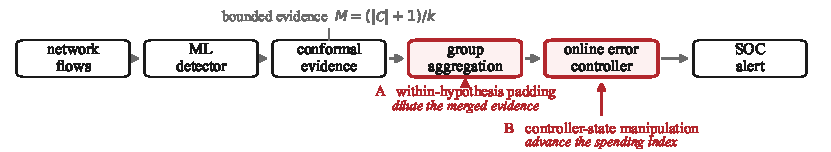
\includegraphics[width=\textwidth]{fig1_system.pdf}
\caption{The statistical trust layer, and the two places an adversary reaches it. Evidence
entering the controller is bounded by $\ceil=(\lvert\Cal\rvert+1)/k$, which \cref{sec:feasibility}
shows creates a finite discovery horizon. Surface~A attacks a hypothesis's \emph{composition}: the
grouping key is made of fields the adversary chooses, so it adds ordinary flows to its own episode,
diluting the merged evidence (\cref{sec:paddingcost}). Surface~B attacks the controller's
\emph{sequential state}: a procedure escaping the horizon by conditioning its spending index on observed
evidence exposes that index to whoever generates the evidence (\cref{sec:state}). Neither requires model
or detector access, or any perturbation of the attacker's own flows.}
\label{fig:system}
\end{figure*}

%% Record: sec 2.1-2.3, 4.13, 4.20.

\subsection{Pipeline and conformal evidence}

\Cref{fig:system} shows the composed system. Flows $x_1, x_2, \ldots$ arrive in timestamp order; a
detector $f$ scores each $s_t = f(x_t)$, and a calibration set $\Cal$ of scored
\emph{benign} flows, disjoint from training and preceding deployment, converts scores into evidence.
With $K_t$ the rank of $s_t$ among the calibration scores from the top, the threshold conformal
e-value is $e_t = \frac{\nCal + 1}{k}\,\mathbf{1}\{K_t \le k\}$, with $\mathbb{E}[e_t] \le 1$ under the
null and $p_t = \min(1, 1/e_t)$. It is two-point --- a flow either beats the $k$-th largest calibration
score or not --- so the evidence is \emph{bounded}, by
\begin{equation}\label{eq:ceiling}
\boxed{\;\ceil = \frac{\nCal + 1}{k}\;}
\end{equation}
No flow, however anomalous, exceeds \cref{eq:ceiling}. This is the finite resolution of
\emph{deterministic rank-based} conformal evidence against a finite calibration
set~\cite{vovk2005alrw,hennhofer2026resolution} --- the unsmoothed threshold construction considered
here, not a feature of our detector --- and the quantity the rest of the paper turns on.
Randomising the rank (\cref{sec:smoothing}) removes the floor, at a measured price.

\emph{The calibration premise.} Every guarantee assumes $\Cal$ contains no attack traffic, and
\cref{sec:contamination} measures its worth: \emph{one flow} in the adversarial worst case, since at
$k=1$ the rule is a single order statistic. The tolerable quantity is a count, not a rate --- and
adversarially it is zero.

\subsection{Security-semantic grouping}

A detector predicts on flows; a SOC acts on something larger. We group flows into units $G_j$ and
aggregate their evidence into one quantity $\Ev(G_j)$ per unit, the hypothesis the online procedure
tests. Since LSPR23 provides no usable flow-to-campaign ground truth, the deployable units here are
\emph{episodes} --- host-pair--time-bucket groups --- never incidents or campaigns. Our aggregation is
the arithmetic mean $\Ev(G) = \frac{1}{m}\sum_{i=1}^{m} e_i$, valid at every arity, so \emph{every
procedure comparison and both attacks use this uncapped mean}; a pre-committed cap $\sum e/n_0$ (valid
only for $m \le n_0$) enters only as a competing policy (\cref{sec:transfer}).
The step to a valid group e-value is algebraic for a \emph{fixed} collection, but here the group is
metadata-selected with random arity, and different controllers need different things of it.

\emph{What each controller requires.} e-LOND and online e-BH control $\FDR$ under \emph{arbitrary}
dependence provided each true-null group carries a \emph{marginally} valid e-value,
$\mathbb{E}[\Ev(G_j)]\le1$ --- weaker than the conditions the p-value procedures need (conditional
super-uniformity, independence, monotonicity; ADDIS additionally uniform conservativeness, which
\cref{sec:escapes} shows it lacks here). The guarantee-bearing claims therefore use e-LOND, and the
property to establish is group-level marginal e-validity.

The conditioning must be done \emph{per hypothesis}, not globally, or the attack analysis below does
not go through: a premise stated against one global metadata $\sigma$-field says nothing once the
adversary enriches that $\sigma$-field elsewhere in the stream, because conditioning on more
information can raise a conditional expectation. So for each group $j$ let $\mathcal{M}_j$ be the
$\sigma$-field generated by the pre-committed metadata that determines \emph{that} hypothesis and
nothing else --- the grouping key, the membership indicators $\mathbf 1\{i\in G_j\}$ and arity $m_j$
of $G_j$, its position in the pre-committed order (hence the spending weight $\gamma_j$ it is
offered), and the horizon $T$. It carries no information about any other group's composition. Note
$\gamma_j$, not the level: for e-LOND $\alphat=\alpha\gamma_t(R_{t-1}+1)$ depends on realised past
rejections, which is exactly what the procedure's own proof permits. ``Pre-committed'' means
\emph{chosen before the scores and not score-adaptive}, not statistically independent of them.

\begin{assumption}[Metadata-conditional per-flow validity]\label{assump:groupval}
For every benign constituent flow $i$ of a true-null group $j$, the per-flow e-value satisfies
$\mathbb{E}[e_i \mid \mathcal{M}_j]\le1$; equivalently, for the two-point conformal e-value,
$\Pr(K_i\le k \mid \mathcal{M}_j)\le k/(\nCal+1)$. This is a \emph{sufficient} condition, stronger than
the unconditional $\mathbb{E}[e_i]\le1$ that split conformal supplies (and weaker than the same
requirement against a global metadata $\sigma$-field); it holds when the benign score
is not adaptive to that group's metadata --- e.g.\ conditional exchangeability of calibration and
null deployment scores given $\mathcal{M}_j$ --- a genuine modelling assumption, since endpoint or
service metadata can correlate with the timing and volume features that drive the score.
\end{assumption}

\begin{lemma}[Group-level marginal e-validity]\label{lem:groupval}
Under \cref{assump:groupval}, every true-null group with $m_j>0$ has a marginally valid group
e-value, $\mathbb{E}[\Ev(G_j)]\le1$, for random membership and random arity $m_j$ and under arbitrary
dependence among the $e_i$. The group-level stream is therefore marginally e-valid, exactly what
e-LOND and online e-BH require.
\end{lemma}

Conditioning on $\mathcal{M}_j$, membership and $m_j$ are fixed, so
$\mathbb{E}[\Ev(G_j)\mid\mathcal{M}_j]=\frac1{m_j}\sum_{i\in G_j}\mathbb{E}[e_i\mid\mathcal{M}_j]\le1$,
and the tower property removes the conditioning (\cref{app:proofs}). Within-group dependence is
irrelevant (only linearity is used) and between-group dependence arbitrary (e-LOND's proof needs only
marginal validity).

\emph{Why not calibrate the group directly?} The obvious way to make this hold by construction is
to stop merging per-flow evidence and run split conformal on the \emph{grouped} unit, with the same
protocol on the calibration split; the premise would then be exchangeability of calibration and
benign test \emph{groups}, with no per-flow conditional statement. We build it, and it is worse in
three ways at once (\cref{sec:groupcal}): the premise is discharged but replaced by ordinary group
exchangeability, which arity heterogeneity suggests may be fragile under group-formation shift; the
evidence ceiling falls by the flows-per-group ratio; and the alerting stops entirely
at the primary and replication windows. The last of these needs no view on the premise at all. \Cref{assump:groupval} is what
survives when feasibility is a requirement rather than an afterthought.

Two clarifications keep this honest. First, ``marginal'' is over the test scores \emph{and} the
calibration draw, \emph{not} conditional on the realised calibration set; the Bates calibration-conditional
adjustment (\cref{apptab:bates}) is stronger than e-LOND needs, so we treat it as optional. Second, the
attacked group is a \emph{false null}, and \cref{assump:groupval} --- like e-LOND's FDR proof ---
constrains only \emph{true-null} groups. Padding changes the attacked \emph{non-null} group's
membership and arity (\cref{thm:padding}), but the pads carry its own key, so \emph{under a
key-determined order} they add no hypothesis and leave every true-null group's $\mathcal{M}_j$
unchanged, so \cref{assump:groupval} holds verbatim on the attacked stream.
This is a second, \emph{validity}, reason to fix the within-bucket order by group metadata rather than
by first-flow arrival (\cref{sec:transfer}): an arrival-ordered tie-break lets a pad shift a true-null
group's position, hence its $\gamma_j$ and $\mathcal{M}_j$. The attack therefore exploits a rule valid
under the premise rather than violating it.
Where the premise fails --- \cref{sec:tail} finds the one window (0.85) whose measured benign firing
rate gives $\mathbb{E}[e]\approx51$, refuting even marginal e-validity --- no $\FDR$ guarantee
attaches, and every number there is a measurement against labels. That firing-rate check is a
\emph{diagnostic}: it can refute validity, but a compatible count does not prove it.

\subsection{Online procedures and metrics}

Each procedure offers a level $\alphat$ at step $t$ and rejects when the evidence exceeds
$1/\alphat$. What distinguishes them, for our purposes, is not their $\FDR$ proof but
\emph{what index advances the spending sequence}. \Cref{tab:procedures} maps the procedures we
test on that axis. It is the map that predicts which of them are covered by \cref{thm:family1}
and \cref{thm:family2} and which escape.

\emph{Metrics.} We report $\FDP$ and $\FDR$; malicious-\emph{flow} coverage and \emph{episode}
recall, whose divergence is the subject of \cref{sec:granularity}; alerts issued; and one
feasibility quantity,
\begin{equation}\label{eq:margin}
\text{margin} = \frac{(\nCal+1)\,w_0}{T} - 1,
\end{equation}
the horizon-uniform feasibility slack of a \emph{level-$w_0$} procedure such as LORD++ (LOND/e-LOND
fire for a band where \cref{eq:margin} is mildly negative, their first-step level being
$\alpha = 2w_0$).

The terms the paper holds distinct --- validity, feasibility, detection power, episode
recall, atomic coverage, alert blur, and the two attack costs --- are collected in \cref{tab:terms}.

\emph{Conventions for the results.} Four hold throughout, so we state them once rather than at each
number. First, the per-alert padding cost $r^{\star}$ is an \emph{oracle} bound (it uses the realised
evidence sum and the unperturbed trajectory) and a \emph{lower} bound on what an attacker must spend;
the paper's other attack quantities are not, and each says which it is where it appears --- $G^{\star}$
and $B^{\star}$ are exact closed forms verified by replay, the keyed-hash $N_{50/90/99}$ are empirical
reliability budgets over $400$ draws, and the front-load $L^{\star}$ and the whole-detected-set padding
totals are \emph{upper} bounds. Second, every \emph{headline
absolute result} --- \cref{tab:main} and the operational evaluation --- is reported under the
\textbf{canonical} within-bucket order, a hash of the group's own metadata key, neither attacker-timed
nor detector-favourable (\cref{sec:transfer}). Paired ablations and sensitivity analyses may instead
run under the shipped \textbf{first-flow} arrival order, the \emph{optimistic upper bound over the
orders we audit}, and \emph{every table and figure that does so says so in its caption}. Where a
result is a \emph{contrast} between two procedures on one stream (smoothing, restart, weighting,
controllers) both legs use the same order, so the order shifts the level and not the sign. Third, position \textbf{0.55} is the \textbf{primary analysis window} and \textbf{0.62} the
\textbf{replication window} --- pre-committed as the analysis pair before any tail diagnostic existed,
not selected by one --- while \textbf{0.85} is a \emph{known-invalid} stress-test window whose evidence
is not a valid e-value and which we use only for mechanism and attack-cost measurement
(\cref{sec:method}). Every $\FDR$ statement at \emph{every} window is conditional on
\cref{assump:groupval}: the benign-tail diagnostic refutes 0.85 and cannot establish the other four. Fourth, the feasibility margin depends on $\nCal$, $k$ and $T$ alone, never on the
scores.

%% =======================================================================================
\section{Threat Model}\label{sec:threat}
%% Record: 05_PAPER_CONTRACT.md sec 6.

\textbf{Defender.} Controls the detector, calibration set, grouping rule, evidence construction and
controller, all correctly implemented --- no attack relies on an implementation flaw.
\textbf{Adversary goal.} Suppress the alert on its own activity; secondarily, delay it or silence the
controller for every later hypothesis.

\textbf{Capability.} The adversary generates network flows from compromised or attacker-controlled
hosts. Because the grouping key is $(\mathrm{SrcIP}, \mathrm{DstIP}, \text{time bucket})$, it controls
group membership by construction: ordinary connections to the host it is already attacking, in the same
bucket, land in the same group --- needing no flow crafting, perturbation, or detector access. It may
also create precursor episodes and order its own flows.

\textbf{Knowledge.} \emph{White-box}: $k$, $\nCal$, procedure parameters and controller state.
\emph{Grey-box}: procedure and parameters but not $\nCal$ nor the state --- for \cref{sec:state} a
$\pm33\%$ estimate of $\nCal$ suffices and unknown state costs $\approx\!36\times$ over-provisioning.
\emph{Black-box}: no detector access; ordinary traffic of a chosen volume on a common service.

\textbf{Cost metric.} Padding flows emitted, converted to bytes and rate in
\cref{sec:state}; where estimated from realised detector output it is a \emph{lower bound}.

\textbf{Out of scope.} We exclude poisoning the detector's \emph{training} set, compromising the SOC,
arbitrary modification of stored scores, and any claim that these attacks have been seen in the
wild. \emph{Calibration}-set contamination is in scope (\cref{sec:contamination}): it needs only
that a labeller miss an attack flow.

%% =======================================================================================
\section{When Can an Online Guarantee Produce Any Alert?}\label{sec:feasibility}
%% Record: 4.13 (theorems), 4.20 (escapes), 4.34 (smoothing), 4.35 (restart).

\emph{Known vs.\ established here.} That bounded evidence loses to a shrinking threshold is elementary
and ``$\alpha$-death'' is known, held cured by $\alpha$-investing~\cite{foster2008alpha}. We establish
the exact structural conditions under which procedures fall silent, that the state is \emph{absorbing}
with a cold-start deadline, the scaling $\nCal \ge kT/c_0 - 1$, and that $\alpha$-investing does
\emph{not} cure it here.

\emph{Three feasibility notions, kept distinct.} A step $t$ is \textbf{evidence-feasible} if the
largest admissible evidence can cross the offered threshold ($\alphat \ge 1/\ceil$); a procedure is
\textbf{cold-start feasible through $T$} if a rejection is possible at every $t \le T$ on a
rejection-free prefix; a state is \textbf{absorbing} if, once entered on such a trajectory,
no later observation can produce a rejection.

\subsection{A finite discovery horizon}

The argument is elementary. Evidence is bounded by $\ceil$ and a rejection at $t$ requires
$E_t \ge 1/\alphat$, so a rejection is possible \emph{at all} only if
\begin{equation}\label{eq:feas}
\alphat \ \ge\ \frac{1}{\ceil}.
\end{equation}
Every procedure in the two families below pays its level from a finite budget, so during a
rejection-free run $\alphat$ cannot recover: it decays under a decaying $\gamma$, and is pinned at the
constant cold-start value $c_0/T$ under horizon-uniform $\gamma$. \Cref{eq:feas} therefore has a last
time it holds, after which the procedure is \emph{silent} --- no observation can change its output. The two families cover four of those we test
(LOND, e-LOND, LORD++, e-LORD); SAFFRON sits outside their letter yet does not escape in practice
(\cref{tab:procedures}), and the two genuine escapes --- ADDIS and online e-BH --- are located in
\cref{sec:escapes}: finding them is part of the result.

\begin{proposition}[Multiplicative family]\label{thm:family1}
Let $\alphat = \alpha\,\gamma_t\,g(\mathcal{H}_{t-1})$ with $\gamma \ge 0$,
$\sum_t \gamma_t \le 1$, and $g \le c\,(R_{t-1}+1)^d$ for the rejection count $R$. Since
$R_{t-1} \le t-1$, a rejection is possible at $t$ only if
$\gamma_t\,t^{d} \ge 1/(\alpha c \ceil)$. If $\gamma_t t^{d} \to 0$, the set of such $t$ is
\textbf{finite}; if $\gamma_t t^{d}$ is additionally eventually non-increasing, feasibility ends
at a last time after which no later step is feasible, and the infeasible state is
\textbf{absorbing}.
\end{proposition}

The degree condition is asymptotic and must be checked per procedure. For the horizon-free
$\gamma_j \propto j^{-1.6}$, $\max_t t\gamma_t = 0.4375$ (at $t=1$) with $t\gamma_t \to 0$, so $d=1$
holds; a procedure whose level grew quadratically in the rejection count would escape the argument. The
horizon-uniform $\gamma_t = 1/T$ falls outside the letter of the condition --- $t\gamma_t = t/T$ rises
to $1$ --- but needs none: before any rejection the level is the \emph{constant} $c_0/T$, so
feasibility over the horizon is all-or-nothing and \cref{cor:budget} decides it, while
\cref{thm:family2}, which assumes no monotonicity of $\gamma$, covers the horizon-uniform case
unchanged.

\begin{proposition}[Lag-sum family]\label{thm:family2}
Let $\alphat = w_0\gamma_t + \sum_j a_j \gamma_{t-\tau_j}$ over rejection times $\tau_j < t$
with $0 \le a_j \le \alpha$ for every $j$ (LORD++ has $a_1 = \alpha-w_0$ and $a_j = \alpha$ for
$j\ge2$). During a rejection-free run of length $\Delta$ every lag is
distinct and at least $\Delta$, so, using $\gamma_{t-\tau_j} \le S(\Delta)$ and $a_j \le \alpha$
term by term, $\alphat \le (w_0+\alpha)S(\Delta)$ with
$S(\Delta) = \sum_{d \ge \Delta}\gamma_d$. Since $S$ is non-increasing and
$\sum\gamma < \infty$ implies $S(\Delta) \to 0$, the quantity
$\Delta^{*} = \min\{\Delta : (w_0+\alpha)S(\Delta) < 1/\ceil\}$ is \textbf{finite}, and
because $\Delta$ only grows during a rejection-free run the infeasible state is
\textbf{absorbing} --- with no monotonicity assumption on $\gamma$ itself.
\end{proposition}

\Cref{thm:family1} covers LOND, e-LOND and \emph{e-LORD} (the last via the equivalence
e-LORD $=$ e-LOND under $\gamma_t = \omega_t\prod_{j<t}(1-\omega_j)$~\cite{egai2025}), and
\cref{thm:family2} covers LORD++. We do \emph{not} extend the bound to the remaining e-GAI members ---
e-SAFFRON at $\lambda=0.1$ is a testing level the equivalence does not cover, and mem-e-LORD controls a
different error rate. Both propositions are verified numerically. The result is a precise scope, not a
claim that online FDR ``dies''.

\subsection{Horizon-uniform feasibility bound}

\begin{corollary}\label{cor:budget}
Feasibility over a horizon $T$ with no prior rejections requires $\nCal \ge k/\alpha_T - 1$. Write
$c_0$ for the \emph{cold-start coefficient} --- the constant multiplying $\gamma_T$ in the level a
procedure offers before its first rejection, so $c_0 = w_0$ for a level-$w_0$ procedure such as
LORD++ and $c_0 = \alpha = 2w_0$ for LOND/e-LOND. Under horizon-uniform $\gamma_t = 1/T$, which is
max-min optimal, this is
\[
\nCal \ \ge\ \frac{kT}{c_0} - 1.
\]
\end{corollary}

\begin{corollary}[Calibration-horizon ratio]\label{cor:calhorizon}
Coarsening or refining the alerting unit moves $\nCal$ and $T$ together. If a construction replaces a
calibration set of $\nCal$ units by one of $\nCal'$ units while leaving the horizon at $T'$, it is
feasible only if $\nCal' \ge kT'/c_0 - 1$. The requirement is therefore a \emph{scale-free count
ratio} $k/c_0$ --- $20$ at $k=1$, $c_0 = \alpha = 0.05$ --- independent of the dataset: a deployment
needs $20$ calibration units per hypothesis it intends to test, whatever the unit is.
\end{corollary}

\emph{This is the most portable statement of C1, because a practitioner budgets in it.} Its calendar
form is not scale-free: converting $20$ units per hypothesis into observation time multiplies it by
the rate at which the calibration and deployment windows produce units, so an attack-free observation
period of $8.5$--$47\times$ the deployment span here (through a measured group-rate ratio of
$0.42$--$2.35$) is a property of \emph{this} stream, while the factor $20$ is not.
\Cref{sec:groupcal} is \cref{cor:calhorizon} applied: calibrating the grouped unit directly replaces
$1.8$--$2.4$M flows by $37$--$57$k groups, and $20$ groups per hypothesis is exactly what the
construction cannot supply.

\Cref{fig:envelope} plots this against the horizon. At $k=1$, $w_0 = 0.025$ it is
$6.5\times10^{8}$ calibration flows at LSPR23 scale for $c_0 = w_0$ ($3.3\times10^{8}$ for
LOND/e-LOND, $c_0=\alpha$),
$1.44\times10^{9}$ for one hour of a 10k-flows/s link, $3.46\times10^{10}$ for one day,
and $3.2\times10^{13}$ under horizon-free $\gamma \propto j^{-1.6}$. The windows we evaluate carry
$\nCal$ between $1.81$M and $2.45$M. The same algebra appears in Krönert et
al.~\cite{kronert2024fdr} as $\nCal = \nu m/\alpha - 1$, answering a different question about a
\emph{windowed} procedure's exactness rather than uninterrupted feasibility (\cref{sec:related}).

The squeeze is sharpest at the very start of the stream. Before its first rejection a procedure carries
no history term, so it has only a short \emph{cold-start window} in which a rejection is possible at
all: under $\gamma \propto j^{-1.6}$, the first 18 hypotheses at $\nCal = 10^4$ and 334 at $10^6$ (29 and
515 for LOND/e-LOND), after which the absorbing state of \cref{thm:family1,thm:family2} is entered. At
the $\pi = 10^{-4}$ low-prevalence sensitivity point that window almost always closes empty. The
first true attack is not expected until
index $\approx\!10{,}000$, so a rejection arrives in time to bootstrap the controller with probability
only $\approx\!0.3\%$; the sole alternative, an early false rejection, has probability at most a few
percent ($4.5\%$ for e-LOND, $2.2\%$ for LORD++, in simulation at a stated $\nCal$; the
benign-only arm of \cref{apptab:prevalence} produces no rejection on any stream, but with five
effective windows that is \emph{consistent with} this rate rather than a test of it,
$\Pr(\text{zero}\mid 4.5\%)=0.79$). The published
$\alpha$-death fix does not help, being identical to the base procedure until that first rejection and
weaker after (\cref{tab:procedures}).

\emph{And live-fire prevalence is the optimistic case.} LSPR23 is an exercise: $10.06\%$ of flows and
$0.48$--$0.81\%$ of episodes are malicious, so we sweep prevalence as a \emph{parameter} down to
$\pi = 10^{-5}$ and to zero --- two to three orders below the exercise, and a sensitivity analysis
rather than a claim about any particular SOC's base rate. Thinning malicious
\emph{episodes} to a target rate --- replacing each with benign evidence from the same window, so $T$,
the margin and every survivor's step index are held \emph{exactly} fixed --- separates the two
quantities cleanly: feasibility does not move at all, while at $\pi = 10^{-3}$ e-LOND's mean detections
fall from $0$--$72$ to $0$--$8$ and at $\pi = 10^{-4}$ its probability of \emph{ever} rejecting is
$0$--$40\%$, mostly under $10\%$ (\cref{apptab:prevalence}). Deleting the hypotheses instead --- which
shortens $T$ and \emph{raises} the margin by up to $+0.013$ --- gives the same collapse to within
$0.02$ in that probability, so it is prevalence and not re-indexing that does the work --- a
distinction worth drawing, because deletion \emph{provably can} help: removing a hypothesis shifts
every later one into a higher $\alphat$, so a survivor that could not clear its own step may clear its
new one. The two escapes
collapse with it. \emph{Every detection count in this paper is therefore an upper bound in one more
respect}, and the separation the paper draws between feasibility and detection is visible here driven
by base rate alone: the margin improves while detection goes to zero. This is a sensitivity, not a
full counterfactual --- a genuinely low-prevalence deployment would also have a different detector,
calibration corpus and benign traffic --- and e-TOAD's collapse is measured over fewer draws than the
other two, so it is directional.

\begin{figure}[t]
\centering
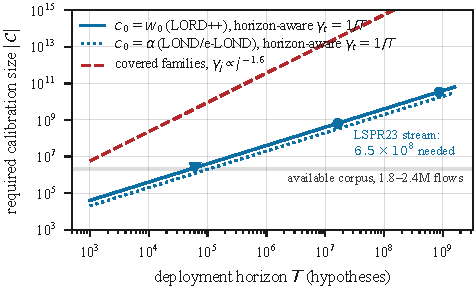
\includegraphics[width=\columnwidth]{fig2_envelope.pdf}
\caption{\textbf{How large must the calibration set be to keep a rejection possible over a
deployment horizon?} At $k = 1$, $w_0 = 0.025$ the requirement $kT/c_0-1$ is linear in $T$ for
every procedure covered by \cref{thm:family1,thm:family2}, differing only through $c_0$ (a factor $2$
between LORD++ and LOND/e-LOND). Online e-BH is plotted for comparison and is \emph{not} covered ---
it escapes the absorbing horizon (\cref{sec:escapes}) --- but still carries a calibration
requirement, linear in $T$ per simultaneous discovery. Both outrun the $1.8$--$2.4$M calibration
flows these windows supply by orders of magnitude.}
\label{fig:envelope}
\end{figure}

\subsection{Which procedures escape, and what the escapes cost}\label{sec:escapes}

Two procedures escape, and among the procedures studied here the boundary is sharp: the horizon binds
a procedure whose spending index advances on \emph{every} hypothesis, and is escaped by one that
advances it only on \emph{tested} hypotheses or defers the decision. This is a classification of
what we examined, not a characterisation of every possible procedure --- \cref{thm:family1} leaves
room for a third route, escape by history-dependent level growth fast enough to outrun $\gamma_t$,
which none of these takes. \emph{ADDIS} takes the first route. Its index counts
hypotheses that are \emph{selected} ($p\le\tau$) but not candidates ($p\le\lambda$), and at $k=1$ no
episode p-value ever lands in $(\lambda,\tau]$, so the index never advances, the level never decays,
and ADDIS is silent $0.0\%$ of the time. But this voids the guarantee: almost no null is selected
(5 of 31,313, first-flow), so its realised $\FDP$ is only what the labels say, and under the max-min-optimal
sequence the wealth discount drops the initial level below the conformal floor, silencing it outright.
\emph{Online e-BH} takes the second: its step-up threshold is a fixed point over the whole
history~\cite{xu2024elond,wang2022evaluebh,fischer2025onlineebh}, so a rejection-free prefix is
simply not absorbing. It still needs the calibration budget ($R$ simultaneous discoveries require
$\nCal \ge T/(\alpha R)-1$), and its advantage is robustness to a misspecified horizon: at the
\emph{stress} window and one seed --- the only cell we sweep the horizon on, so read it as an
illustration of the mechanism rather than a measured rate --- online e-BH keeps $144$ of its $152$
rejections under a $100\times$ over-estimate, where LOND keeps all $151$ at $2\times$ but
\textbf{none} at $100\times$, and LORD++ none already at $2\times$.

\emph{The second route is not one procedure but a one-parameter family, and the parameter is
alerting latency.} Under decision deadlines~\cite{fisher2022deadlines} each hypothesis must be
decided by a time $d_t \ge t$ or accepted for good; $d_t = t$ recovers e-LOND and
$d_t = \infty$ recovers online e-BH~\cite{xu2026eclosure}, so the two ends of the boundary above are
joined by a continuum. Its operational reading is direct --- $d_t$ is how long a SOC will let a
hypothesis sit undecided --- and a bucket-close deadline is exactly the \emph{batched} architecture a
SOC receives, arbitrary-dependence valid where a batched BH is not (\cref{sec:related}).
\textbf{Deferring does not buy feasibility.} Measured exactly, the fraction of hypotheses that cannot
be rejected \emph{at their own arrival} is unchanged by the deadline --- $96.3\%$ at the primary
window whether decisions are immediate, held to bucket close, or never forced ($90.1\%$ under
first-flow arrival; \cref{apptab:uai26}) --- because reaching a step-up count of $R$ needs $R$
hypotheses to clear the bar at once, and on our streams at most $0.48\%$ of episodes carry
any evidence at all. The
escape works by \emph{revisiting}, so it is paid in latency --- and under the order \cref{tab:main}
reports it buys almost nothing. Across the ten window--seed cells, deferring to bucket close converts
to power at \textbf{exactly one}, and there it buys \textbf{one} detection ($34\to35$ at $0.85$), the
\emph{known-invalid} window whose evidence is not a valid e-value anyway. Under first-flow arrival ---
the optimistic bound --- it converts at two cells ($13\to32$ at $0.62$, $30\to31$ at $0.70$) and at
none of the other eight. \emph{Latency is a lever on the controller, not on the evidence.}

\emph{Do the newest procedures escape the cold-start barrier?} No. The strict improvements over
e-LOND published under arbitrary dependence --- a closure construction and a compound-e ``donation''
construction, two recent strict improvements directly applicable to our
setting~\cite{xu2026eclosure,xu2025closure} ---
fail to reach a first rejection before it, for two different reasons.

\begin{proposition}[Donation is bounded before the first rejection]\label{prop:donation}
For donation e-LOND with parameter $\delta\in(0,1]$, on a rejection-free prefix,
$\alphat \le \delta\gamma_t/(1-\delta)$. Hence donation e-LOND satisfies \cref{thm:family1} with
$c = 1/(1-\delta)$, $d = 1$: the horizon stays finite and the infeasible state absorbing.
\end{proposition}

The mechanism is one line: donation's wealth is $\gamma$-weighted and $\sum\gamma\le1$, so \emph{the
donation budget is the spending budget}, and redistributing wealth cannot manufacture it. At
$\delta=\alpha$ the cold-start coefficient moves only from $\alpha$ to $\alpha/(1-\alpha)$ --- the
calibration requirement shrinks by a factor $(1-\alpha)$, i.e.\ $5\%$, against a shortfall of
$20\times$ (\cref{cor:calhorizon}). What \cref{prop:donation} establishes is therefore precisely this: \emph{donation cannot rescue a
controller that fails to obtain its first rejection before the bounded-evidence cold-start horizon}. It
is not a global cap and must not be quoted as one --- after $1/\delta$ rejections the denominator can
vanish and the level is not bounded by this expression at all --- and it is sharp where it applies. Runs here \emph{do} pass that
count --- $30$, $31$ and $73$ rejections at $0.70$, $0.77$ and $0.85$, where the realised boost
reaches $1.83$ against the cold-start ceiling $1.05$. What we observe is the weaker and sufficient
fact that the denominator never actually vanishes on these streams, the realised donation wealth
staying at most $0.12$ of a budget of $1$.

\begin{proposition}[Closure is bounded by its zero-evidence subset]\label{prop:closure}
For closed e-LOND, let $Z_t = \#\{i<t : E_i = 0\}$. Then $\alphat \le \delta\gamma_{Z_t+1}(R_{t-1}+1)$.
\end{proposition}

\begin{corollary}[When the closure is absorbing]\label{cor:closureabsorb}
If along a rejection-free run $Z_t\to\infty$ fast enough that $\gamma_{Z_t+1}\to0$, closed e-LOND
enters the absorbing infeasible state. Two sufficient conditions, one finite and one asymptotic. Let
$H = \min\{j:\gamma_j < 1/(\delta\ceil)\}$ be \cref{thm:family1}'s index horizon.
\emph{(i)} With $P_T = \#\{i\le T: E_i>0\}$ the number of hypotheses carrying \emph{any} evidence,
the run is absorbed by step $H + P_T$ whenever $H+P_T\le T$ --- an \emph{additive} offset, holding
pathwise along the rejection-free run with no assumption beyond counting.
\emph{(ii)} Asymptotically, if $\liminf_t Z_t/t > 0$ then for \emph{every}
$\rho'<\liminf_t Z_t/t$ the horizon is eventually \cref{thm:family1}'s rescaled by $\rho'$.
\end{corollary}

This is a genuinely new covered case rather than an instance of \cref{thm:family1} --- the closure's
level is not $\gamma_t$ times a bounded factor --- so C1's scope widens rather than merely extending.
The zero-evidence hypotheses form an \emph{admissible subset}, giving the same decay under a rescaled
index. The \emph{bound} is unconditional; the \emph{conclusion} is not, and \cref{cor:closureabsorb}
carries its hypothesis. Form \emph{(i)} is the one that applies here, and it needs no density
argument: a stream carries $P_T$ hypotheses with any evidence at all, and the closure cannot outrun
its own index by more than that many steps. Our streams make the offset small --- $P_T$ is $0$ to
$152$ across the ten window--seed cells, at most $0.48\%$ of $T$ --- so the closure's horizon exceeds
\cref{thm:family1}'s by at most $152$ hypotheses and the cap is attained. Where instead most
hypotheses carry positive evidence $P_T$ approaches $T$, $Z_t$ stays small and the bound says little:
that is the regime the closure was designed for, and it is not the sparse-evidence regime studied
here. Both proofs are in \cref{app:proofs}. The r-LOND variants inherit the classification
verbatim: their rejection sets coincide with the e-LOND ones on calibrated $p$-values.

Measured, under the canonical order the two buy $+0$ and $+0$ true detections across ten
window--seed configurations, and $+1$ and $+0$ under first-flow arrival (\cref{apptab:uai26}),
because these streams have almost no evidence to redistribute. The barrier
is a property of the evidence, not of the controller's sophistication. For e-TOAD we use the
interpretation of the active set and the step-up upper limit that is consistent with the stated limiting
cases; the alternate literal interpretation is included as a sensitivity analysis and does not affect our
conclusion (\cref{apptab:uai26}).

\begin{table*}[t]
\centering
\caption{Main cross-window results, detector seed 0 (the ten-row two-seed matrix is in
\cref{app:matrices}). Two-hour host-pair grouping, e-LOND, $\gamma \propto j^{-1.6}$, $k=1$,
$q = 0.05$; margin is \cref{eq:margin}. ``Detected'' is e-LOND true-positive rejections under the
\textbf{canonical} metadata-hash order, with the shipped first-flow order --- an optimistic
\emph{upper bound over the orders we audit} --- beside it (\cref{sec:transfer}); ``median pad'' is the black-box suppression
cost of the canonical detections against the \emph{running} level $1/\alphat$, a lower bound.
\textbf{0.55 is the primary analysis window, 0.62 the replication window} --- pre-committed, with every
$\FDR$ statement at all five conditional on \cref{assump:groupval,lem:groupval}.
\textbf{0.85 is the known-invalid stress-test window}, its benign tail an unambiguous \emph{violation}
($\mathbb{E}[e]\approx51$); the other four are merely \emph{not refuted} by a diagnostic resting on
$0$--$3$ benign firings (\cref{apptab:tail}), and the metadata-stratified reading is not clean at any
(\cref{apptab:a1strata}).
Position 0.70 carries the feasibility-is-not-detection separation: at seed 1 the same $+0.536$ margin
with AUROC $0.914 \to 0.847$ takes first-flow detections from 30 to \textbf{0}, and the canonical
order gives \textbf{0} at both seeds. The canonical column is one draw from the $50$-order ensemble
(medians $1$, $6$, $2.5$, $1$, $23.5$; maxima $10$, $11$, $12$, $6$, $44$), and not a uniformly
typical one: it sits above the ensemble median at $0.55$, $0.62$ and $0.85$ --- \emph{at} the maximum
at $0.62$ --- and below it at $0.70$ and $0.77$. The first-flow column exceeds every ensemble maximum
(\cref{apptab:ordering}).}
\label{tab:main}
\begin{tabular}{lrrrrrrrrl}
\toprule
 &  &  &  &  & malicious & \multicolumn{2}{c}{canonical order} & first-flow & tail vs.\ \\
Position & AUROC & $T$ (episodes) & $\nCal$ & margin & ep.\ & detected & median pad & (upper bd.) & nominal \\
\midrule
0.55 & 0.916  & 57{,}368 & 2{,}448{,}993 & $+0.067$ & 275 & 3  & 24    & 18 & compatible ($1.07\times$) \\
0.62 & 0.799  & 49{,}267 & 2{,}449{,}031 & $+0.243$ & 398 & 11 & 6     & 13 & compatible ($1.16\times$) \\
0.70 & 0.914  & 37{,}231 & 2{,}287{,}988 & $+0.536$ & 287 & 0  & ---   & 30 & compatible ($3.79\times$) \\
0.77 & 0.828  & 31{,}672 & 2{,}116{,}418 & $+0.671$ & 246 & 0  & ---   & 31 & compatible ($2.72\times$) \\
0.85 & 0.999  & 31{,}568 & 1{,}813{,}113 & $+0.436$ & 255 & 34 & 116   & 72 & \textbf{violated} ($50.9\times$) \\
\bottomrule
\end{tabular}
\end{table*}

\subsection{Removing the premises: smoothing and restart}\label{sec:smoothing}\label{sec:restart}

Both premises are load-bearing, and removing either carries a measured cost (\cref{app:boundary}).
\emph{Randomised smoothing} replaces the discrete p-value with a $\mathrm{Unif}(0,1)$
draw~\cite{vovk2005alrw,hennhofer2026resolution} and dissolves the absorbing state --- but the extra
detections are a lottery. \emph{Both legs of this contrast, and of the restart and weighting contrasts
below, run under first-flow arrival} --- the order shifts the level an alert fires at, not the sign of a
paired comparison (\cref{sec:transfer}). At the primary window smoothed LOND rejects $24.1{\pm}2.7$
episodes against $18$ discrete, yet the set detected \emph{reliably} (probability $\ge0.9$) is still
those same $18$, and the surplus does not survive arbitrary-dependence-valid merging (Hommel gives
$12.5$). \emph{Restart} instead buys back real power, and its design chooses the cost: resetting the
budget each epoch raises recall from $0.065$ to $0.345$ but forfeits the deployment-wide guarantee ($\FDR = 1-(1-q)^n$ grows with
the epoch count), while pre-allocating it ($\sum_i q_i\le q$) keeps deployment-wide $\FDR\le q$ at some
of that power (recall $0.195$; \cref{apptab:restart}). Restart forces a power-versus-guarantee choice,
then, rather than voiding the guarantee.

%% =======================================================================================
\section{The Granularity--Guarantee Tradeoff}\label{sec:granularity}
%% Record: 4.9, 4.29, 4.35, 4.38.

\Cref{cor:budget} makes the exchange rate explicit: since $\nCal_{\min} = kT/c_0 - 1$ in the
cold-start coefficient $c_0$ ($=\alpha$ for the e-LOND controller we report), grouping buys
feasibility \emph{directly} by reducing $T$ from $T_{\text{flows}}$ to
$T_{\text{episodes}}$ --- an exact lockstep, not a heuristic improvement. We
test five families a SOC would recognise (source--dest host pair, source host, dest host, /24 subnet
pair, source--service), each over six bucket widths from five minutes to one day plus a whole-deployment
bucket --- 35 configurations in all (\cref{app:matrices}).

\subsection{The empirical granularity curve}

Two things happen as the unit coarsens (\cref{fig:granularity}).

\emph{Feasibility is bought exactly.} The required $\nCal$ is linear in $T$ in every family, so each
becomes feasible once the bucket is coarse enough. Source-host grouping is feasible at \emph{every}
bucket, collapsing each window to $763$--$24{,}043$ episodes and needing well under the
$1.8$--$2.4$M calibration flows available --- and an attacker-host alert is an ordinary SOC unit, so the
barrier \emph{can} be bought off.

\emph{Resolution is what pays.} Against a \emph{fixed atomic reference} --- the 5-minute src-dst
malicious episodes --- each issued alert blurs from $1$ of them to $\sim\!20$--$40$ as the bucket
coarsens (\cref{fig:granularity}), localising the attack to a day-long host-pair blob. Episode recall
(moving denominator) also falls under the oracle sequence ($0.66\to0.49$ at 0.85), but its direction is
$\gamma$-dependent, so we rest the cost on the blur.

\emph{That atom is our own unit, so we tested it against one we did not choose --- and report what
that test can and cannot support.} LSPR23 ships the red team's task record: $288$ tasks, $295$
timestamped step submissions, an \emph{attacker-defined} decomposition of the same campaign. The
tasks' declared network segments are the dataset's own per-flow \texttt{seg} vocabulary under a
constant prefix, corroborated against the machine-readable compromise reports ($83$ agree, $0$
disagree). Counting distinct red-team \emph{steps} merged into each issued alert, the external count
\textbf{rises with the alerting unit as the proxy does}: at $0.70$ it runs $4.3\to27.0$ across
$5$\,min--$24$\,h buckets against the proxy's $1.0\to28.3$ (rank agreement $+1.000$ over six widths,
$+0.800$ under the canonical order, $+0.816$ at $0.77$). \textbf{But we do not claim this as
corroboration}, for three measured reasons (\cref{apptab:semblur}). \emph{(i)} A null that rotates the
red-team timeline against the stream --- preserving task identity, ordering and inter-arrival
structure --- reproduces the observed counts at $18$ of $19$ cells: the rise is driven by the bucket
width capturing more submissions, not by alert-level correspondence. \emph{(ii)} The record sees the
alerts at only $3$ of $10$ window--order cells, and the reason is \cref{thm:family1} again --- issued
alerts sit in the feasible prefix, the \emph{first minutes} of a deployment window, and at $0.55$ and
$0.62$ that predates the exercise's first submission, so only $2\%$ of alerts overlap it in time at
all. \emph{An external record can only speak about an alert it coincides with, and the feasibility
boundary puts the alerts where the record is silent.} \emph{(iii)} Every attributed alert sits on a
labelled-malicious episode and the labels came from this same exercise, so nothing here is
label-independent evidence that an alert is a true positive. Two further limits: the whole result
rests on \textbf{six} coarse segment labels --- across every row the compromise-IP conjunct admits no
alert the segment conjunct did not --- and at the $24$\,h bucket both nulls tie the observation
because every submission shares one bucket, so only sub-daily widths inform. The honest reading is
that the external unit \emph{agrees in direction} and is \emph{too coarse to discriminate}: the resolution cost survives
the substitution but is not independently confirmed by it.

\emph{Malicious-flow coverage is not a clean measure of the resolution cost}, which is why the
exchange rate does not rest on it. It is dominated by the traffic mass of whichever episodes happen to
fire --- the top three host pairs carry $45$--$87\%$ of malicious traffic --- so it swings by orders of
magnitude both across windows and with the bucket (\cref{apptab:w7coverage}). We therefore report it
per configuration and rest the resolution cost on the blur.

\begin{figure}[t]
\centering
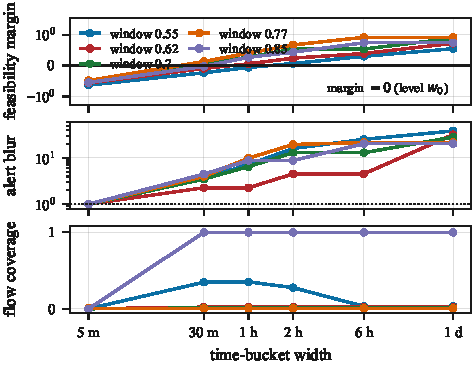
\includegraphics[width=\columnwidth]{fig3_granularity.pdf}
\caption{Per-window granularity for the source--dest pair unit (five windows, seed 0). Coarsening the
bucket buys feasibility (top: margin rises through zero) and costs resolution (middle: \emph{alert blur}
--- fixed 5-minute reference units per alert --- climbs from $1$ to $20$--$40$). Malicious-flow coverage
(bottom) is \emph{not} a clean resolution measure: set by whether the window's dominant episodes fire, it
varies across windows \emph{and} with the bucket (\cref{apptab:w7coverage}).}
\label{fig:granularity}
\end{figure}

Coarsening is not the only lever: periodic restart (\cref{sec:restart}) divides the hypothesis count a
run must survive, preserving episode resolution (hourly restart at one-hour grouping reaches recall
\textbf{0.406} at $\approx\!125$ alerts against \textbf{0.103} for six-hour coarsening). The tradeoff
is granularity against the \emph{form} of the deployment-wide guarantee; the exchange rate above
concerns a single uninterrupted controller.

%% =======================================================================================
\section{The Statistical Trust Layer as an Attack Surface}\label{sec:attack}
%% Record: 4.16 (theorem), 4.30 + t46 (real cost, placement), 4.36 (asymmetric),
%% 4.33 (ADDIS state), 4.40 (operational units), 4.42 (cross-window).

\Cref{sec:granularity} showed that aggregation is the direct route to feasibility. The catch is that
both the aggregation and the adaptive state that lets a procedure escape \cref{thm:family1,thm:family2}
are reachable by an adversary who only generates traffic --- no detector access, no crafted flows.
\textbf{Surface~A} is a practical, low-footprint \emph{evasion}: suppressing the alert on one's own
episode costs tens of ordinary flows at the primary window (a median of $24$ under the order we
report, $118$ under the detector-favourable one). \textbf{Surface~B} is a
\emph{structural controllability} result about one of the escapes: an attacker who manufactures evidence
advances a spending index that is conditioned on that evidence, and drives it to permanent failure. It
is conspicuous in volume rather than cheap ($37.5\times$ the window's traffic; \cref{sec:state}), and it
coincides with Surface~A wherever ADDIS's cap binds (\cref{sec:coincide}). Online e-BH escapes by a
different mechanism, which we do not attack.

\subsection{Attack surface A: within-hypothesis padding}

Group evidence is $\Ev(G) = F(e_1, \ldots, e_m)$. Under the two-point construction an ordinary flow
that does not reach the $k$-th calibration rank contributes e-value \emph{exactly} $0$, so an
adversary who appends $r$ such flows to its own group makes the controller evaluate
$F(e_1, \ldots, e_m, 0^r)$ --- ``padding'' throughout means appended zero-evidence flows.
Nothing about the detector changes: the malicious flows still individually exceed the ceiling.
The attack is aimed at the trust layer, not the classifier, and is available to anyone who can open
ordinary connections. We consider three merging classes: the symmetric mean (a valid e-merging family at
every arity, the subject of \cref{thm:padding}); the pre-committed cap $\sum e/n_0$ (valid \emph{only}
for $m \le n_0$); and pre-committed asymmetric position-weighted rules (\cref{sec:asymmetric}).

\subsection{Symmetric padding impossibility}

\begin{definition}[$\tau$-padding-robustness, attainment]
A family $\{F_N\}_{N \ge 1}$ of e-merging functions is $\tau$-padding-robust, for $\tau > 1$,
if for every $m \ge 1$, every finite $x \in [0,\infty)^m$ with $F_m(x) \ge \tau$, and every
$r \ge 0$, $F_{m+r}(x, 0^r) \ge \tau$; it \emph{attains} $\tau$ if some finite input has
$F_m(x) \ge \tau$.
\end{definition}

Attainment rules out a vacuous escape: without it the definition is satisfied by rules that never
reach $\tau$, such as $F \equiv 1$, which can never fire since rejection needs evidence
$\ge 1/\alphat > 1$.

\begin{theorem}[Symmetric padding impossibility]\label{thm:padding}
No family of symmetric e-merging functions that attains $\tau$ is $\tau$-padding-robust, for
any $\tau > 1$. Quantitatively, for every symmetric e-merging family, every finite
$x \in [0,\infty)^m$ and every $\tau > 1$,
\[
F_{m+r}(x, 0^r) < \tau \qquad\text{whenever}\qquad r > \frac{\sum_i x_i}{\tau} - m.
\]
\end{theorem}

\begin{proof}[Proof sketch]
Vovk and Wang's Proposition 3.1~\cite{vovk2021evalues} shows the arithmetic mean
\emph{essentially} dominates any symmetric e-merging function: $F(e) > 1$ implies
$M_K(e) \ge F(e)$ on finite inputs. Ordinary domination is false ($\lambda + (1-\lambda)M_K$
is a counterexample), so it is used through a case split, giving
$F_N(x) \le \max(1, \mathrm{mean}(x))$. Padding gives
$\mathrm{mean}(x, 0^r) = (\sum x)/(m+r)$, which falls below $\tau$ once
$r > (\sum x)/\tau - m$; attainment supplies an $x$ with $F_m(x) \ge \tau$. The full proof, a
tightness argument, and an independent special case needing no domination result are in
\cref{app:proofs}.
\end{proof}

Since rejection requires evidence $\ge 1/\alphat$ with $\alphat < 1$, the threshold is
\emph{always} $\tau > 1$, so \cref{thm:padding} applies to every rejection threshold any
valid online procedure can set. The one symmetric rule that resists it is the pre-committed cap
$\sum e / n_0$: valid and padding-robust within its cap, but not an e-merging family above $n_0$ ---
its validity \emph{is} the condition $m \le n_0$ --- and below the cap strictly
dominated by the mean. It escapes by being inadmissible, and the power it forfeits is a measured
detection loss (\cref{sec:transfer,app:attacks}).

\emph{And appending is not the only lever.} \Cref{thm:padding} is about \emph{appending} to a
hypothesis, so a statistic that appending cannot lower --- the group \textsc{max} of
\cref{sec:groupcal} --- resists it outright. It does not resist the complementary move: \emph{creating}
hypotheses ahead of the target, which appends nothing and pushes it out of the cold-start window past
which no rejection is possible. Because group-level calibration shrinks the ceiling, that window
collapses from $748$--$902$ steps to $65$--$86$, and every group-\textsc{max} detection falls to
$62$--$295$ inserted hypotheses (\cref{apptab:insertion}). Getting ahead of a target is free under
first-flow arrival; under a \emph{public} hash it costs an offline search we price at
$1.0\times10^{4}$--$1.8\times10^{5}$ candidate keys, on three conditions we state rather than assume --- a public
seed, enough endpoint pairs the adversary can actually send between, and a stable key encoding, which
our cache's category codes are not; under a \emph{keyed} hash the ranking cannot be computed offline
at all, so the adversary must insert \emph{blind} --- and we measure what that costs
(\cref{apptab:blindkey}). \emph{The seed does not stop the attack}: all $84$ detections across the
window--order cells that detect anything fall in \emph{every} draw at a budget of $10^{6}$ keys. What
it changes is the currency. A public hash buys the ranking offline for free and instantiates only the
$G^{\star} = 30$--$813$ keys that land ahead; a keyed seed forces the adversary to instantiate
\emph{every} trial as real traffic between distinct endpoint pairs, and at matched reliability that is
\textbf{$2.1$--$89\times$ more host pairs (median $19\times$)} --- $N_{99}$ runs to $3.4\times10^{4}$.
\textbf{That cost is a capability, not a computation}, and the result assumes an adversary who has it:
$N_{99}$ counts endpoint pairs it must actually be able to originate traffic between, so on a network
where only a few hundred reachable pairs are available to it the seed is not a partial mitigation but
a hard stop --- which is the regime in which a keyed hash is worth most, and which our cost figures
should not be read as covering.
\emph{A keyed canonicalization is therefore a genuine partial mitigation for targeted insertion, and it
does nothing whatever to Surface~A padding}, which needs no key at all. \emph{Validity by design plus padding
robustness therefore does not buy attack resistance --- it buys resistance to one attack while making
the other far cheaper.} On the shipped pipeline the two levers split: insertion beats
padding for one alert at \textbf{none} of the twelve window--order cells, but silences the entire
controller for $217$--$813$
hypotheses against $80$--$7.9\times10^{8}$ flows to pad every detection separately --- the latter an
\emph{upper} bound, since suppressing an early rejection lowers $R$ and can make the rest cheaper or
moot, and heavy-tail driven at its extreme (at $0.85$ ten of $72$ pad costs carry almost all the sum).
Per episode the targeted insertion cost is $434$--$5{,}674$ hypotheses, which is why padding wins
there.

\subsection{Real-network suppression cost}\label{sec:paddingcost}

On real traffic (\cref{fig:attacks}A), priced against the \emph{running} level $1/\alphat$ at each
detected episode's step, suppressing a detected alert is \emph{cheap}: under the canonical order the
medians are $24$, $6$ and $116$ flows at the three windows that detect anything --- $0.55$, $0.62$
and the known-invalid $0.85$, the dearest of the three being the one that carries no guarantee ---
over $n=3$, $11$
and $34$ individually-priced episodes, so read the first two as prices rather than as rates
(the three at $0.55$ cost $23$, $24$ and $33$) --- and under the
first-flow upper bound --- which detects more episodes, deeper into the level sequence --- $118$, $72$,
$1{,}851$, $1{,}165$ and $5{,}202$, heavy-tailed to $10^{7}$--$10^{8}$ for late, low-$\alphat$ alerts.
The order changes \emph{which} episodes survive to be attacked, not whether they can be: across $50$
orders the per-order median stays at $16$--$178$ flows across both detector seeds. Pricing against the static $\tau = T/w_0$ ---
the first-step level, a conservative stand-in for e-LOND's cheaper $T/\alpha$ --- is the cheap extreme
(median $34$ flows at 0.85 under the canonical order, $33$ under first-flow); we report the
larger running-level cost.

The realism of the padding barely matters. Four of the five pools (generic benign, attacker-origin,
protocol-matched, black-box) coincide within a few percent at each window
(\cref{tab:pools}), because the running level (median $\sim\!10^{4}$--$10^{6}$) dwarfs the largest pool
mean ($216.8$); only service-matched is $1.4$--$2.0\times$ dearer. The black-box pool uses
network-observable frequency alone --- the most common $(\text{proto},\text{port})$ over the traffic
\emph{preceding} deployment, with no labels or detector output --- so it is the \emph{weakest}-attacker
rule, yet also the correct one: taking the mode over the deployment window would instead pick the
attacker's own flood, which does not dilute (\cref{apptab:w3dilution}).

Two attacker capabilities must be kept apart. \emph{Constructing} the pad is black-box: it needs no
detector access, only an ordinary service the victim answers (0 firings in 20{,}000). \emph{Sizing} it
to the minimal $r^{\star}=\lfloor S\alphat\rfloor-m+1$ is not --- that uses the realised evidence sum
$S$, the running level, and the unperturbed trajectory --- so every reported $r^{\star}$ is an
\emph{oracle} lower bound. A grey-box attacker who knows the design but not the live state must
over-provision: since $1/\alphat$ spans $\sim\!10^{4}$--$10^{6}$ within a window, a fixed budget $Y$
suppresses exactly the alerts with $r^{\star}\le Y$, so guaranteeing an arbitrary one requires
budgeting for the tail --- equally for every pool, so pool-insensitivity stands.

\subsubsection*{Can the attacker put the pad flows where they have to go?}

The episode key is $(\mathrm{SrcIP}, \mathrm{DstIP}, \text{bucket})$, so a pad must land on \emph{the
target's own host pair} --- the attacker sends ordinary traffic to the host it is already attacking.
A label-matched pool cannot be built here (all \textbf{310} host pairs carrying any malicious flow are
\textbf{100\% malicious}), but structure settles the \emph{endpoint} question: the detector reads
\texttt{Protocol} and 32 timing/volume statistics but \emph{no} endpoint identity, so endpoint identity
cannot affect the score. What it does \emph{not} settle is response-dependent transfer --- 17 of 33
features are backward or bidirectional --- so whether an ordinary flow of a service the victim answers
transfers is \emph{empirical}. \textbf{We test it directly:} $20{,}000$ real black-box-service flows
through the shipped detector fire \textbf{0} (a one-sided $95\%$ upper bound of $1.5\times10^{-4}$ on
the firing rate), and injecting them dilutes $E(G)=S/(m+r)$ to suppression at exactly the closed-form
$r^{\star}$ on \textbf{every} detection under \emph{both} orders --- $3/3$ and $34/34$ under the
canonical order the paper reports, $18/18$ and $72/72$ under the first-flow upper bound
(\cref{apptab:w3dilution}). The canonical arm is the one that carries the argument, since only there
does padding provably leave every other $\mathcal{M}_j$ untouched (\cref{sec:transfer}); the
first-flow arm shows the result is not an artefact of the smaller set.

\subsection{Does the attack transfer? A second detector and a second dataset}\label{sec:transferattack}

The suppression above is scoped to \emph{flow-level} features, so we probe that scope. First we build
the host-conditioned detector the boundary calls for --- six strictly-causal host-context features on a
second, \emph{higher-AUROC} detector ($0.954$ vs $0.916$; \cref{apptab:r7host}). It sharpens C1: the
higher AUROC buys \emph{fewer} e-LOND detections (2 against 18, both first-flow), so ranking quality and operational
alerting move in opposite directions. The transfer still holds at both windows --- replaying the append
causally, black-box pads fire zero and the cost stays the flow-level closed form ($r^{\star}=108$ against
$118$, both under first-flow arrival, the order that experiment runs under) --- but LSPR23 cannot settle the benign-inclusive question, its attacked pairs being $100\%$
malicious.

We therefore re-measure on AIT-LDSv2.0~\cite{aitlds}, whose eight organisations serve real
benign-to-victim traffic. The \emph{full} Surface~A chain --- leave-one-org-out flow detector, in-org
benign calibration, e-LOND, and suppression by \emph{replaying real} benign flows --- suppresses
\textbf{78 of 79} detected episodes under the canonical order (\texttt{russellmitchell} excepted), and
\textbf{84 of 85} when the same folds are resequenced by first-flow arrival (\texttt{santos} excepted;
\cref{apptab:aitorder}); a cross-organisation host detector adds only a weak signal ($8.9\%$ on
\texttt{shaw}). \textbf{Host conditioning does not stop the attack
once the pad's own context is modelled}: recomputing the six features as pads accumulate, all nine
host-conditioned detections across \texttt{shaw} and \texttt{wilson} suppress
(\cref{apptab:r7host,apptab:r7ait,apptab:aitsupp}; boundary limits in \cref{sec:limitations}).

\subsection{Can asymmetric aggregation fix it?}\label{sec:asymmetric}

The natural escape is to abandon symmetry: a
pre-committed, position-indexed weighting $F(e) = \sum_i w_i e_i$ is valid under arbitrary
dependence whenever $\sum_i w_i \le 1$~\cite{wang2025admissible}, and is padding-invariant by
construction. Two exact bounds close it.

\begin{theorem}[Reach]\label{thm:reach}
For a pre-committed weight sequence with $\sum_i w_i \le 1$, the number $P$ of positions at which a
lone attack flow can fire the rule is \emph{at most} $\alphat \ceil$ --- the same quantity that governs
the feasibility horizon of \cref{cor:budget}.
\end{theorem}

\begin{theorem}[Front-load cost]\label{thm:frontload}
The number of leading zero-evidence flows that make detection impossible is
$L^{*}(w) = \min\{L : \sum_{i>L} w_i < \beta\}$ with $\beta = 1/(\alphat \ceil)$, which is
\emph{finite for every summable $w$}.
\end{theorem}

\Cref{thm:frontload} is the same summable-tail lemma as \cref{thm:family2}, on the
within-episode position axis rather than stream time --- one result on two axes, which is why no
choice of weights escapes: the design sets only the price, and it is paid out of power.

Measured at the primary window (\cref{tab:asym}), \emph{every} padding-invariant scheme that retains
the mean's recall is defeated by \textbf{1 to 8 leading flows}, against $111$ appended for the symmetric
mean on the same episodes --- $14$--$112\times$ cheaper (buying more robustness, $L^{*}$ up to 164,
forfeits $\sim\!58\%$ of the recall, first-flow on both legs); the stress window has the same shape. Two schemes fail
structurally: last-event-only is not padding-invariant, and a security-prior port weighting is
\emph{out of class} and fires on none of the 275 episodes. So a pre-committed scheme cannot have
padding invariance, usable power, and ordering robustness at once --- validity forces $\sum w\le1$,
\cref{thm:reach} caps the reach, \cref{thm:frontload} makes $L^{*}$ finite. The asymmetric escape only
converts appended padding (hundreds to thousands of flows) into front-loading (one to a few hundred);
it does not stop the attack.

\subsection{Attack surface B: controller-state manipulation}\label{sec:state}

\Cref{sec:escapes} showed that ADDIS escapes the feasibility horizon because its spending index
counts hypotheses that are \emph{selected but not candidates}, which threshold conformal evidence at
$k=1$ never produces here. That escape is what exposes it: an adversary who manufactures
episodes with $p \in (\lambda, \tau]$ advances the index at will, and such episodes are never
rejected, so they cost it no discoveries of its own.

\begin{theorem}[ADDIS state budget]\label{thm:addis}
Under $\gamma_j = (j+1)^{-1.6}/\zeta(1.6)$ (ADDIS's $0$-indexed sequence), $k$-th-rank conformal
evidence, and precursors injected at index $D=0$, $B^{*}$ is the smallest $D$ with
$D + 1 > \left[(\tau-\lambda)W(\nCal+1)/(k\,\zeta(1.6))\right]^{1/1.6}$, where $W = w_0$ before
the first rejection and $W = \alpha R$ after $R$ of them.
\end{theorem}

Verified against the implementation on the real stream at position $0.85$, the
\emph{known-invalid} window --- necessarily so, for the reason two paragraphs below
(\cref{fig:attacks}B): \textbf{$B = 202$
precursor episodes leave all 152 rejections intact, and $B = 203$ leaves none} --- permanently, an
absorbing state of exactly the kind ADDIS was designed to avoid. The attack survives the
grey-box setting: the admissible group size is a $\tau/\lambda$-wide interval, so a
$\pm 33\%$ estimate of $\nCal$ suffices and unknown controller state costs only $36\times$
over-provisioning.

\emph{Does this reach online e-BH?} No: it escapes \cref{thm:family1,thm:family2} by a fixed point over
the whole history, not a spending index, so there is nothing for injected evidence to advance. Whether
some other manipulation of its fixed point exists is open; the result here is about the
index-conditioning mechanism, exemplified by ADDIS.

\emph{Is this an artefact of the invalid window?} ADDIS's horizon-escape on two-point conformal
evidence is \emph{inseparable} from its guarantee-invalidity: the spending index fails to advance
precisely when the p-values never land in $(\lambda,\tau]$, the same reason they are not uniformly
conservative --- so no such stream is both escape-feasible and guarantee-valid. We therefore confirm
the mechanism on a synthetic stream with genuinely conservative $\mathrm{Unif}(0,1)$ nulls, where
ADDIS's guarantee holds (empirical all-null $\FDR = 0.010 \le q$; \cref{apptab:addissynth}). The attack is then adversarial \emph{state poisoning} --- injecting
admissible \emph{alternative} precursors (non-null, so ADDIS's true-null assumption is untouched and its
guarantee holds on the attacked stream) --- and still drives every detection to silence, at a median
$B^{\star}=140$ over 300 guarantee-valid streams (range $140$--$255$, the tail from a rare null false
positive that transiently restores wealth). The security consequence is a property of the mechanism,
not of the 0.85 window's validity failure.

\textbf{The price is set by the calibration budget, not any implementation weakness.} One precursor
must be a group large enough that its single firing clears $\lambda$ ---
$\lfloor\lambda(\nCal+1)/k\rfloor + 1 = 453{,}279$ flows --- so silencing the controller costs
$9.2\times10^{7}$ flows, scaling as $\lambda\nCal\,[(\tau-\lambda)w_0\nCal]^{0.625}/k^{1.625}$. The same
quantity that buys feasibility buys resistance to the state attack.

\textbf{In operational units, the attack is conspicuous, not cheap.} Those 92 million flows are 36.1 GB
over position 0.85's 2.4-hour span --- \textbf{33.4 Mbit/s}, four hosts at 10 Mbit/s each. What makes it
structural is its volume against the monitored population: $37.5\times$ the window's entire flow count,
$5.6\times$ the whole dataset. Suppressing one e-LOND alert, by contrast, costs a median $116$ flows
under the canonical order --- $4.7\times10^{-5}$ of the window's traffic, almost \emph{six} orders of
magnitude below, and $5{,}202$ flows ($2.1\times10^{-3}$, four orders) under the first-flow upper
bound.

\subsection{The two attack surfaces coincide}\label{sec:coincide}

ADDIS caps its level at $\lambda$ and the state-advancement window \emph{starts} at $\lambda$, so
wherever the cap binds the cheapest suppressing pad also advances the spending index (101 of ADDIS's
147 true detections): the state attack comes free with the padding one (cap-saturation \emph{implies}
landing; \cref{app:proofs}). It is also \emph{cheaper} against ADDIS, whose level is five orders of
magnitude above e-LOND's --- padding one episode costs a median $3.4\times10^{7}$ flows, so state
manipulation wins from the third episode on. The large per-hypothesis level that makes ADDIS escape is
what makes it cheap to defeat through the state that maintains it: a design lesson, not a theorem for
every procedure.

\begin{figure*}[t]
\centering
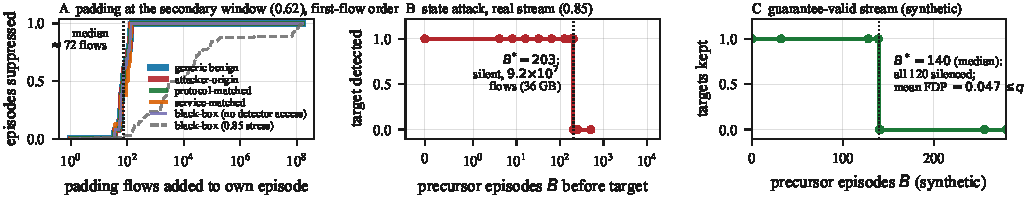
\includegraphics[width=\textwidth]{fig4_attacks.pdf}
\caption{\textbf{What does each attack cost?} \textbf{A}: suppressing one alert at the
\emph{replication} window (0.62) is a low-footprint evasion, insensitive to pad realism; the costs
plotted are the \textbf{first-flow} arrival arm --- the optimistic upper bound over the orders we
audit, and the more expensive one for the attacker --- over that order's $13$ detections. Under the
canonical order \cref{tab:main} reports, the same window detects $11$ episodes at a median of $6$
flows each (\cref{tab:pools}). \textbf{B}: permanently
silencing ADDIS through its adaptive state (0.85 stress) is conspicuous in volume, at exactly the
\cref{thm:addis} threshold. \textbf{C}: the same poisoning on a synthetic stream where ADDIS's
guarantee genuinely holds still silences every detection.}
\label{fig:attacks}
\end{figure*}

%% =======================================================================================
\section{Experimental Methodology}\label{sec:method}
%% Record: sec 3 (data), 4.15 (protocol), 4.12/4.25 (caps), 4.38 (selection protocol).

\subsection{Dataset and protocol}

\textbf{LSPR23}~\cite{lspr23}, captured at Locked Shields, the largest live-fire cyber-defence
exercise: 16,353,511 flows over 161.5 hours, 1,644,599 of them malicious (10.06\%; $0.48$--$0.81\%$
of \emph{episodes}) --- a live-fire base rate that \cref{sec:feasibility}'s prevalence sweep prices as
an \emph{optimistic} bias rather than leaving as a caveat. The stream is
timestamp-sorted before any split, and 89\% of flows fall in the final 25.6 hours, so window
positions are chronological slices rather than random splits. It carries no
flow-to-campaign labels --- \texttt{Expoid\_dst} is empty for 1,630,732 of the 1,644,599 malicious
flows, and \texttt{Category}, \texttt{Severity} and \texttt{SigID} are effectively constant where
present, one code covering $99.98\%$ of the labelled rows --- which is why our units are episodes. A separate red-team task record (288
narratives, 83 machine-readable compromise reports, 295 timestamped step submissions) is external
ground truth for the alert audit of \cref{sec:tail} only, never a feature.

\emph{Chronological protocol.} Training, then calibration, then deployment, no leakage. Fixed-size blocks (calibration
15\%, test 15\% of $N$) are slid to five positions along the sorted stream, so $T$ and $\nCal$
vary because the \emph{traffic} differs, not the window sizes. Benign subsampling is
confined to training. Two detector seeds per position vary the scores while leaving $T$ and $\nCal$
untouched, so the feasibility margin is seed-independent by construction and seeds are never pooled.
Across positions, $\nCal$ runs 1,813,113--2,449,031.

\emph{Which windows carry the headline numbers, and why that is not a validity claim.} \textbf{0.55 and
0.62 were pre-committed as the primary and replication windows} before any benign-tail diagnostic
existed; no post-hoc rule selects them, and we do not invent one. The diagnostic runs in the other
direction, and it is weak by construction: the entire split rests on \textbf{$0$--$46$ benign
firings} out of $1.6$--$2.3$M ($1$, $1$, $3$, $2$, $46$ at seed 0; \emph{zero} at two windows on
seed 1), so at 0.55 the exact Clopper--Pearson interval on the measured/nominal ratio is
$[0.03, 5.96]$ --- an interval that excludes essentially nothing. Four
positions are \emph{not refuted} ($1.07$--$3.79\times$, every interval containing $1$;
\cref{apptab:tail}), which is a failure to reject and not support. Position 0.85 alone is a clear
violation ($50.9\times$, interval $[37.3, 67.9]$), so it is the \emph{known-invalid} stress-test
window, used only for mechanism and attack-cost measurement. Accordingly \textbf{every
guarantee-bearing statement in this paper, at every window, is conditional on \cref{assump:groupval}}
--- the window names mark which stream carries which headline number, not which stream has been
empirically validated.

\subsection{Detectors and procedures}

Detector novelty is not a contribution: the detector is HistGradientBoosting, and every detection,
attack and coverage number is its output. An unsupervised Isolation Forest runs alongside as a
\emph{feasibility-vs-sufficiency} probe --- same feasibility margin (a function of $\nCal,k,T$ alone),
yet tail reach \textbf{0.000 at all ten configurations}: not one attack flow outscores all
$1.8$--$2.4$M benign calibration scores. \emph{Feasibility is necessary, not sufficient}; since it
never detects, the attack results are statements about the HistGradientBoosting pipeline.

\emph{Procedures.} LOND, LORD++, e-LOND, SAFFRON, ADDIS, online e-BH, and the e-GAI family (e-LORD,
e-SAFFRON, mem-e-LORD), transcribed from primary sources and unit-tested against literal $O(T^2)$
implementations and four identities the papers state. Throughout $\alpha = q = 0.05$, $w_0 = 0.025$,
$k = 1$, ADDIS $\lambda = 0.25$, $\tau = 0.5$; each $\gamma$-procedure runs two spending sequences:
$\gamma_j \propto j^{-1.6}$ (no horizon) and horizon-uniform $\gamma_j = 1/T$ (max-min optimal, needs
the stream length, labelled \oracle).

\subsection{Grouping and reproducibility}

\emph{The online stream.} A group's evidence uses every flow in its time bucket, so its hypothesis is
emitted only when the bucket \emph{closes}, using only observations available then; no group is decided
using a flow outside its own closed bucket. Groups closing in the same bucket are sequenced by a
pre-committed, evidence-independent key, and that tie-break is a \emph{choice} with consequences
(\cref{sec:transfer}). We report the \textbf{canonical} choice --- a splitmix64 hash of the group's own
$(\mathrm{SrcIP},\mathrm{DstIP},\text{bucket})$ key, collisions broken on the key --- which reads no
arrival time, so padding an episode moves no other group's slot and \cref{assump:groupval} is provably
undisturbed by it. The initial first-flow arrival order is reported alongside as an
optimistic upper bound over the orders we audit.

The headline grouping is $(\mathrm{SrcIP}, \mathrm{DstIP}, \text{2-hour bucket})$ with the
uncapped arithmetic-mean rule; the capped $\sum e/n_0$ rule enters only in the cap-policy analysis.
This is a deployable configuration, not an oracle optimum, and is not tuned on the reported window: it
is in fact near-\emph{worst} among the feasible groupings under previous-window selection, the cap
being the selection-stable choice while the grouping does not transfer (\cref{sec:transfer}), and the
feasibility gate precedes selection, being a function of $\nCal$, $k$ and $T$ alone.
Every result is computed on the full stream; each closed form is verified
numerically against an independent implementation, and each measurement script carries unit tests.

%% =======================================================================================
\section{Operational Evaluation}\label{sec:operational}
%% Record: 4.19 (frontier), 4.24 (q vs gamma), 4.14 + 4.39 (feedback).

\subsection{The point the controller chooses, and its cost}

Comparing a $q=0.05$ procedure against an arbitrary classifier threshold measures nothing, so we place
every method on the achievable frontier of the episode-max-score threshold family at its own budget ---
an \emph{ex-post oracle} (its thresholds use the test labels) that bounds what the \emph{ranking} admits
(\cref{apptab:frontier,apptab:frontier85}), \emph{under the canonical order the headline uses}. The
frontier is itself order-free --- it is a threshold family on the episode max score --- which we verify
rather than assume, since its tie-break is by stream position; only the controller rows move. The result
is a clean negative: every method sits within $0.047$ recall of the best achievable point at its budget,
the informative comparisons being the $\FDP>0$ rows.

The comparison that matters is thus \emph{choice of point}, not efficiency, and the canonical order
sharpens it. At the primary window e-LOND operates at \textbf{3} alerts, recall $0.011$, $\FDP\,0.000$
(18 and $0.065$ under first-flow arrival), while an ex-post oracle at the \emph{same} zero error reaches
recall $0.378$ on 104 alerts --- \textbf{thirty-five times} as much, against six under the optimistic
order: a measure of how far below the ranking's ceiling the $\alpha$-wealth process sits, and one the
ordering objection makes larger rather than smaller. And the lever that moves the point is not
operational: sweeping $q$ twenty-fold moves median recall by $0.088$, while switching the spending
sequence at fixed $q$ moves it by $0.188$ ($5.8\times$ the alert count) --- a first-flow paired sweep,
both legs on the same stream. Formal error control can
therefore \emph{reduce} the operator's freedom over the workload--recall tradeoff. \emph{Closing the
loop does not rescue this unless labels arrive in minutes}: the three feedback \emph{threshold
controllers} (P, PI, AQT; \cref{app:procedures}, first-flow) reach $\FDP\,0.402$ (P, PI) and $0.523$ (AQT) at
fifteen-minute disposition delay, agree with one another by four hours, and reach the no-feedback threshold
($0.841$) only by eight (\cref{apptab:feedback}) --- a
statement about \emph{delay} on these controllers, not about feedback-driven testing in general, for
which folding revealed labels into the threshold with finite-sample control
retained~\cite{lu2026gaif} is the principled construction whose input our measurement prices.

%% =======================================================================================
\section{Robustness and Failure Analyses}\label{sec:robustness}
%% Record: 4.31 (tail), 4.32 (audit), 4.37 (contamination), 4.41 (ties), 4.38 (transfer).

\subsection{Calibration validity and the labels}\label{sec:tail}

Calibration drift is mild almost everywhere. The measured-to-nominal firing ratio stays near one
across our ten position$\times$seed configurations (median $1.94\times$; independently $0.86$--$2.03\times$
on the AIT \texttt{wilson} testbed~\cite{aitlds}), with a single exception --- the stress-test window
0.85, where the benign firing rate runs $50.9\times$ nominal, so $\mathbb{E}[e]\approx51$ and the
evidence is not a valid e-value there. The excess is sharply localised: three host pairs carry 44 of
the 46 firing benign flows, and removing them restores the ratio to $2.22\times$. It is best explained
by label error, which the alternatives --- distribution shift, a new benign mode, duplicated records,
Mondrian conformal --- each fail to account for (\cref{app:quality}), though we do not prove it.

\emph{The marginal rate is the weakest possible evidence for \cref{assump:groupval}, so we interrogate
it conditionally.} We stratify the firing benign flows on the observable components of $\mathcal{M}_j$
--- arity (what padding moves), service, bucket, and destination host --- and read them at rank depths
$k\in\{1,\dots,1000\}$, resampling both the shared calibration tail and the test side
(\cref{apptab:a1strata}). The result cuts both ways. At the depth the pipeline uses ($k=1$) the data
mostly cannot speak: at the shipped depth $129$ of $134$ strata carry no test at all ($428$ of $536$
cells across the four depths), and none that are estimable reject at a
primary window --- an \emph{inconclusive non-rejection}, not support. Deeper in the tail it is
another matter: $32$ contrasts survive correction at \emph{all five} windows ($25$ after removing the
one confounder we can identify), the strongest an arity bin at $0.77$ --- uncomfortable, since arity is
what padding moves. But a departure at $k=1000$ is compatible with a valid rank-1 rate, and no finite
sample identifies a conditional expectation, so we draw the conservative conclusion: the
guarantee-bearing claims stay stated \emph{under} \cref{assump:groupval}, not supported by this
diagnostic.

Two consequences follow. First, the guarantee does not attach at 0.85, so that window serves only for
mechanism and attack-cost measurement; the feasibility horizon (\cref{eq:feas}) is unaffected, not
depending on the evidence at all. Second, every $\FDP$ there is measured against labels: auditing the
ADDIS ($\gamma\propto j^{-1.6}$) set's 152 alerts against the red team's task record, 146 agree ($96.1\%$) and six
disagree, so an under-estimate is not excluded. e-LOND's realised $\FDP$ is $0.0066$ (frozen) or
$[0,0.0265]$ (strict post-hoc); the audit is partly circular (99 of 152 verdicts rest on the
label-generating identities), so it indicates the error's direction, not a value. Two of the audit's
four indicators are not discriminative --- temporal concurrency separates $100.0\%$ of alerts from
$86.0\%$ of non-alerted benign episodes --- so only the strict rule's two branches carry weight.

\emph{What \cref{assump:groupval} does and does not govern.} It is worth separating this once,
because the three results of this paper do not stand or fall together.
\textbf{(1) The feasibility theorems need no distributional premise at all.}
\Cref{thm:family1,thm:family2,cor:budget,cor:calhorizon} are statements about a level sequence against
a bounded evidence ceiling; they hold whatever the evidence distribution is, valid or not, and
\cref{eq:margin} is a function of $\nCal$, $k$ and $T$ alone. C1 is therefore untouched by any reading
of this diagnostic.
\textbf{(2) \Cref{thm:padding} is an aggregation theorem, not a data assumption.} It is a statement
about symmetric $e$-merging functions --- that no such function which can fire is invariant to
appended zero-evidence arguments --- and it is proved from admissibility, with no reference to how the
evidence was generated. C2's impossibility half is likewise independent.
\textbf{(3) Only the $\FDR$ numbers on the empirical stream are conditional on \cref{assump:groupval}}:
the realised $\FDP$s, the guarantee-bearing reading of any of them, and \cref{lem:groupval}'s
marginal validity.
Those are the claims that carry the premise, and the ones we mark accordingly throughout.
And the construction that would discharge (3) by design is priced in (1): calibrating the grouped unit
directly replaces \cref{assump:groupval} with ordinary group exchangeability and then, by
\cref{cor:calhorizon}, cannot supply the calibration it needs --- an infeasibility that holds however
the premise is resolved (\cref{sec:groupcal}).

\subsection{Calibrating the group directly}\label{sec:groupcal}

The diagnostic interrogates \cref{assump:groupval}; the constructive alternative is to remove the
need for it, by running split conformal on the grouped unit --- same key, same protocol, on the
calibration split --- so that only calibration/test \emph{group} exchangeability is required. Built
and measured over two group statistics, five windows and two seeds, it fails all three counts a
repair must meet (\cref{apptab:groupcal}).

\emph{The repair really does discharge \cref{assump:groupval}}: the premise becomes ordinary
calibration/test \emph{group} exchangeability, and the group statistic's dependence on arity does not
by itself contradict that --- a statistic may be strongly arity-dependent while calibration and null
test groups remain perfectly exchangeable. Two things qualify it, and neither is a refutation. \emph{Group exchangeability is
still a deployment assumption}, and our threat model is one under which the test groups are partly
adversary-constituted: insertion instantiates endpoint pairs that enter the stream as \emph{true
nulls}, so the group-formation process itself is something the adversary moves. (Padding does not
bear on it: it enlarges the \emph{attacked} group, which is a false null, and the premise constrains
only true nulls.) That is a reason the assumption may be fragile under group-formation shift, not a
proof that it fails. And \emph{the
\textsc{max} statistic makes that fragility acute} --- its rank correlation with arity is
$+0.23$--$+0.41$ across the ten window--seed cells, and within the calibration set groups above a
thousand flows contribute $3.6$--$15.3\%$ of their own bin to the top $1\%$ against $0.26$--$0.44\%$
for singletons. That is a decomposition of the calibration set, and marginally $1\%$ by construction, so
it settles nothing on its own; scoring benign \emph{test} groups against the calibration threshold does.
Marginal coverage is roughly right ($0.55$--$2.32\times$ nominal over the ten cells), while
\emph{arity-conditional} coverage is not: strata run from $0.13\times$ to $\mathbf{24.2\times}$ nominal
under \textsc{max} against $0.00$--$5.6\times$ under the mean. The guarantee is marginal over an arity
mix, and arity is the stratum the adversary chooses.
Stratifying calibration on arity restores a per-stratum guarantee and leaves each stratum a cold-start
window of $2$--$52$ hypotheses. \emph{The robustness and the fragility are one fact}: appending cannot
lower a maximum, which is why \cref{thm:padding} does not run against it and why the arity dependence
is there at all --- while the \emph{mean}, arity-invariant to within noise ($-0.12$ to $+0.09$), is
exactly the rule \cref{thm:padding} defeats.

\emph{Grant the repair its validity premise, then: it still cannot alert.} Group calibration replaces $1.8$--$2.4$M \emph{flows} with $37$--$57$k
\emph{groups}, so $\ceil$ falls $40$--$49\times$ at unchanged $T$: the margin moves $+0.067 \to
-0.977$, no window is feasible, and detection at the primary and replication windows falls from $18$ and $13$ to
\textbf{zero}. That is the boundary, not a weak statistic --- at $0.55$ the cold-start window is $81$
hypotheses while the first of $110$ firing groups arrives at position $401$, and feasible-step counts
match $\lfloor(\alpha\ceil(R{+}1)/\zeta(1.6))^{1/1.6}\rfloor$ everywhere, $0.85$ included, where $42$
detections are the bootstrap ($10.5\times$) on evidence that is not a valid e-value anyway. By
\cref{cor:calhorizon} that is $20$ groups per hypothesis the construction cannot supply. Two scope
notes: calibration groups containing any malicious flow are excluded, which drops up to $26.1\%$ of
calibration flows, in groups whose mean arity runs up to $45.4\times$ the benign mean --- a bias that
favours \emph{firing}, so the negative result survives its own bias; and the worst arity bin reaches
$15.3\times$ nominal.

\subsection{Calibration contamination}\label{sec:contamination}

At $k = 1$ the conformal rule is one order statistic, the calibration maximum, so contamination
acts only through it. Injecting $j$ attack flows above that maximum hands the threshold to the attacker
once $j \ge k$, so tolerable adversarial mislabels are exactly $k-1$, and feasibility has fixed
$k=1$. \textbf{One} mislabelled flow above the calibration maximum takes episode recall to
0.000, from $0.011$ at $0.55$ and $0.133$ at $0.85$ under the canonical order ($0.065$ and $0.282$
under first-flow arrival; the mechanism is order-free, the recall it destroys is not). A \emph{random}
mislabel is milder but not much: median recall $0.004$ at $0.55$ and $0.035$ at $0.85$, with zero
recall in $22.5\%$ and $32.25\%$ of draws, of scale $\varepsilon^{*} = 1/(N q_0) =$
\textbf{1.11--1.31 flows}. Contamination tolerance is a count, not a rate, and adversarially zero.

A second channel runs the other way, and gently: a contaminating flow \emph{below} the calibration
maximum only inflates the p-value denominator, degrading the guarantee to at most $q(1+\varepsilon)$ ---
doubling $q$ would take a contaminating set the size of the calibration set. So \emph{power dies at one
flow while validity barely moves.} And the \emph{feasibility margin is not a safety indicator}: across
the sweep that destroys detection it does not move at all ($+0.436$ throughout, while recall
falls $0.133\to0.000$ canonically, $0.282\to0.000$ under first-flow); it rises to $+0.556$ only in a
separate below-threshold injection that leaves every detection standing.

\subsection{Order robustness and configuration selection}\label{sec:transfer}

Ordering is robust to timestamp ties (at most 1.3\% of episodes share a first timestamp; all 36
reported statistics are invariant across 50 randomised within-timestamp orders).

\emph{The within-bucket order, by contrast, is load-bearing --- and it is where \cref{thm:family1}
becomes visible.} Since $\alphat$ decays with step index and evidence is capped at $(\nCal{+}1)/k$,
only a prefix can reject at all: $902/902/865/824/748$ steps at the five windows, \textbf{$1.6$--$2.6\%$
of the stream}. A detection therefore needs a near-ceiling episode to land inside it --- which under
first-flow arrival is exactly what live-fire attack traffic does. Sequencing the same episodes by their
own metadata instead takes the counts from $18/13/30/31/72$ to $3/11/0/0/34$, and at $0.70$ and $0.77$
\emph{no} episode clears its own step anywhere in the stream. \emph{The ordering result and the
feasibility theorem are one finding measured twice}: three detections out of $275$ malicious episodes
at the primary window is \cref{cor:budget}'s $20\times$ shortfall seen from the detection side. Over
$50$ pre-committed orders the count has median $1$ here and $23.5$ at the stress window; the canonical
order is not a uniformly typical draw from that ensemble --- above its median at three windows, at its
maximum at $0.62$, below it at the two where nothing detects --- while first-flow matches or exceeds its maximum at
every window and seed --- strictly, except where nothing detects at all
(\cref{apptab:ordering}).

\emph{Why that canonical order.} First-flow arrival is an attacker \emph{timing lever} --- delaying an
episode's first flow pushes it to a later, lower-$\alphat$ slot --- and the damage escapes the
attacker's own hypothesis: one pad at the start of its bucket moves \textbf{373} \emph{other} episodes
here, shifting the $\gamma_j$ (hence the $\mathcal{M}_j$) each is offered. A tie-break reading only the
group's \emph{own} $(\mathrm{SrcIP},\mathrm{DstIP},\text{bucket})$ key makes that \textbf{0} by
construction, so \cref{sec:background}'s \cref{assump:groupval}-preservation argument now describes the
order the paper \emph{reports}, not one it merely recommends. Three qualifications, all measured rather
than assumed away. It removes the \emph{timing} lever, not the \emph{metadata} one: the sort key is
own-key-only, so \emph{appending} flows moves no other group, but a group's absolute rank still depends
on which other keys exist, and an adversary that \emph{creates} keys moves ranks. A \emph{public} hash
is moreover grindable over the attacker-selectable $(\mathrm{SrcIP},\mathrm{DstIP})$ --- with the
feasible prefix at $1.6$--$2.6\%$, an adversary trying $100$ candidate keys lands one inside it with
probability $0.80$--$0.93$, and \emph{avoids} it on the first draw with probability $\ge 0.974$; the
canonical order is therefore a \emph{canonicalization, not a security mechanism}. A \emph{keyed} hash
removes grinding, at the price of a seed the adversary can neither learn nor infer --- one our published
seed does not instantiate. It is a real but partial defence: blind insertion still suppresses every
detection, at $2.1$--$89\times$ the instantiated-key cost (\cref{sec:attack,apptab:blindkey}). And it
is not free of power: one keyed instance detects \textbf{0} here.

The frozen configuration is not tuned on its reported window: under previous-window selection and five
leave-one-out folds it is near-\emph{worst} of the $30$ groupings feasible at every window
(of $35$ in the grid), and the cap transfers across
windows while the grouping does not (worst normalised regret $0.070$ vs $0.991$). The cap is
deliberately the validity-and-cost choice, not the powerful one.

\subsection{What did not work}\label{sec:negative}

Several natural alternatives fail: inflation and fragmentation (per-group evidence is flat in group
size), boosting ($b^{*}=1$ for two-point evidence), raising $k$, smoothing, asymmetric weighting,
stratified (Mondrian) conformal, and the published $\alpha$-death fix --- each for the reason given in
\cref{app:negative}.

%% =======================================================================================
\section{Discussion}\label{sec:discussion}

\emph{What should a practitioner do?} \textbf{If deployment-wide $\FDR$ matters}, treat
\cref{cor:budget} as a sizing requirement: the calibration corpus is linear in the hypothesis count,
unattainable at flow granularity, so choose the alerting unit first and the procedure second.
\textbf{If fine resolution matters}, restarting restores detection but promises only a per-epoch
guarantee (or deployment-wide at less power) --- the SOC should be told which. \textbf{If grouping is
used}, treat the aggregation rule as adversarially exposed, and fix the within-bucket order by group
metadata rather than arrival. \textbf{If analyst labels arrive quickly} (minutes, not hours), feedback control is reasonable, but the
construction to reach for folds labels into the threshold with error control
retained~\cite{lu2026gaif}, not a bare threshold controller. And because these observations are
attacker-generated whenever the grouping key is attacker-choosable, any adaptive mechanism that
conditions future behaviour on observed data --- aggregation and controller state alike --- must be
threat-modelled.

\emph{Scope.}\label{sec:nonclaims} We do not claim online $\FDR$ control is unusable, that dependence
breaks it (e-values remove that), or that generic drift invalidates conformal evidence; nor that a
better detector cannot help --- detector quality \emph{cannot} change C1's margin, though it can change
power. Four things we specifically do \emph{not} claim: that the conformal-resolution incompatibility
was itself unknown (C1 characterises \emph{when} it becomes structural~\cite{huo2024realtime}); that
Surface~B reaches online e-BH; that host-aware detection is no defence against padding in general; or
that \cref{assump:groupval} is established rather than assumed.

Four scope statements attach to specific results and travel with them.
\emph{(i)} \Cref{prop:donation} bounds donation's level \emph{before the first rejection} only; past
$1/\delta$ rejections the level is not bounded by that expression at all, and the bound must not be
quoted as a global cap. Runs here \emph{do} pass that count; what holds instead is the weaker
and sufficient fact that the denominator never vanishes on these streams (\cref{sec:escapes}).
\emph{(ii)} For e-TOAD's decision-deadline construction we use the interpretation consistent with the
stated limiting cases ($d_t = t \Rightarrow$ e-LOND, $d_t = \infty \Rightarrow$ online e-BH); the
alternate literal interpretation is included as a sensitivity analysis (\cref{apptab:uai26}) and does
not affect our conclusion.
\emph{(iii)} One equation of the compound-e construction admits two readings --- the rejection history it
scores is not nested, so a literal snapshot and a running union differ. We report both and default to the
literal one; the choice does not affect our conclusion.
\emph{(iv)} The canonical within-bucket order is a \emph{canonicalization, not a security mechanism}:
the insertion attack survives both a \emph{public} hash, which is grindable, and a \emph{keyed} one,
which is not --- under a secret seed the attack costs $2.1$--$89\times$ more \emph{instantiated}
endpoint pairs but still succeeds. That measurement assumes the target sits in the first bucket of its
window, which holds at every cell here; where an earlier bucket exists the adversary inserts there and
precedes the target with probability one.

\subsection{Limitations}\label{sec:limitations}

\textbf{A single live-fire dataset.} Five window positions are five quasi-independent deployments of
one exercise, not five datasets; a triage of $\approx\!40$ public datasets against two catalogues found
none with a genuine flow-to-campaign identifier, complete negatives and recoverable
order, so our units are episodes. \textbf{Position 0.85 is not a valid-e-value window}:
every $\FDP$ there is measured against labels, and the audit indicates but does not
prove an over-estimate. \textbf{\Cref{assump:groupval} is assumed, not established}: the
metadata-stratified diagnostic fails to reject it at the shipped depth --- where $129$ of $134$
strata cannot be tested at all --- but finds the conditional statement measurably imperfect deeper in
the tail, at every window (\cref{apptab:a1strata}). It is nonetheless a \emph{priced} choice rather
than a convenience: the construction that would discharge it silences the primary and replication
windows outright, whatever one grants about the premise it substitutes (\cref{sec:groupcal}). We do not claim to have exhausted the
alternatives --- a two-way calibration split isolating granularity from the group statistic, and
grouping keys the adversary cannot choose, are both untested. \textbf{Per-alert padding costs are oracle lower bounds}, and the other attack quantities are
labelled where they appear rather than covered by that phrase (\cref{sec:background}); the state
attack's absolute cost is
dataset-specific in $\nCal$ and window span, its closed form is not.

\textbf{Padding placement is scoped to flow-level features} (\cref{sec:transferattack}): the full
Surface~A chain suppresses $78$ of $79$ real detected episodes across the eight AIT organisations under
the canonical order ($84$ of $85$ under first-flow), and
on the nine host-conditioned detections we replay end-to-end, conditioning does not stop it once the
pad's own context is modelled --- but we do \emph{not} claim host-aware detectors are no defence in
general, since the accumulation model pins distinct-peer counts (padding from \emph{new} hosts is
uncovered), the six features are one design, and the high-volume flood regime is untested.
\textbf{Scope of C1}: discrete evidence, an uninterrupted controller, two covered families.

%% =======================================================================================
\section{Related Work}\label{sec:related}

\textbf{Online FDR and $\alpha$-investing.} LORD, LOND, SAFFRON, ADDIS, e-LOND and online e-BH
establish stream
validity~\cite{javanmard2015lond,javanmard2018lord,ramdas2017lordpp,ramdas2018saffron,tian2019addis,xu2024elond,wang2022evaluebh,fischer2025onlineebh},
building on $\alpha$-investing~\cite{foster2008alpha}, safe testing~\cite{grunwald2024safe} and offline
$\FDR$~\cite{benjamini1995controlling}. ``$\alpha$-death''~\cite{ramdas2017lordpp} is held cured by
$\alpha$-investing; it is not cured here (the published fix~\cite{egai2025} equals e-LORD before the
first rejection). \textbf{Recent procedures directly applicable to our setting} --- strict
improvements over e-LOND and r-LOND under \emph{arbitrary} dependence, built from an online e-closure
principle and from compound e-values~\cite{xu2026eclosure,xu2025closure} --- are classified against C1
in \cref{sec:escapes} rather than merely cited: neither rescues a controller that fails to obtain its
first rejection before the bounded-evidence cold-start horizon, which is what makes C1 a statement about
the evidence rather than about a particular controller's vintage.

\textbf{Batching.} A SOC receives a batch when a time bucket closes, so a batched procedure is the
natural architecture, and batching is known to recover power and stabilise
ordering~\cite{zrnic2020batching}. We do not use BatchBH or its relatives because their guarantees
need independence or positive dependence \emph{within} the batch, which co-located flows sharing hosts
and one calibration tail cannot supply --- the reason the pipeline is built on e-values at all. The
batched alternative that survives arbitrary dependence and applies directly here is a bucket-close
decision deadline,
which we run (\cref{sec:escapes,apptab:uai26}); and batching with a \emph{deployment-wide} budget obeys
\cref{cor:budget} unchanged, since allocating $\sum_b \alpha_b \le \alpha$ across batches reproduces the
same exchange rate. Batching escapes the horizon only by resetting the guarantee per batch, which is
our restart escape under another name (\cref{sec:restart}).

\textbf{Conformal resolution meets online testing: the nearest prior work.} Conformal
prediction~\cite{vovk2005alrw} and conformal p-values for outlier testing~\cite{bates2023outliers}
supply the evidence, with a calibration-conditional adjustment for small-$k$ failure. Resolution
collapse under discrete conformal evidence was studied in a batch setting with smoothing as the
remedy~\cite{hennhofer2026resolution}, and batching framed as power recovery~\cite{zrnic2020batching};
our restart analysis instead prices the guarantee's composition.
\textbf{The collision our C1 must be positioned against} is Huo et al.~\cite{huo2024realtime}, who
state that conformal p-values are bounded below by $1/(\nCal+1)$, which ``leads to unsatisfactory
performance for online multiple testing methods based on p-values'', and who observe $\alpha$-death
empirically for LOND, SAFFRON and ADDIS on conformal evidence, easing as $\nCal$ grows, responding with
a local-$\FDR$ selection rule rather than a compositional analysis. The \emph{phenomenon} is thus
known; what C1 adds is \emph{when it stops being a power loss and becomes structural} --- the finite
absorbing horizon, exchange rate, escape classification and escape costs of \cref{sec:intro}, for two
families covering the e-value procedures as well as the p-value ones. Krönert et
al.~\cite{kronert2024fdr} come closest in \emph{form}, requiring $\nCal = \nu m/\alpha - 1$ for a
windowed BH --- our \cref{cor:budget} algebra --- but to make that \emph{windowed} procedure's realised
level exact, tuning $\nCal$ upward for power; ours is the threshold below which no rejection is possible
at all, over an uninterrupted horizon rather than a sliding window (their windowing is our restart
escape, \cref{sec:restart}).

\textbf{Trustworthy ML intrusion detection, and online conformal-FDR pipelines.} TESSERACT~\cite{pendlebury2019tesseract}
sets the temporal-evaluation constraints our protocol respects, and
Transcend(ent)~\cite{jordaney2017transcend,barbero2022transcendent} apply conformal calibration with
rolling recalibration. Closest to ours are pipelines that \emph{compose} conformal evidence with
sequential false-discovery
control~\cite{rebjock2021online,farzaneh2025coad,wang2025multilayer,caliburn2026}, with Gao et
al.~\cite{gao2026boundary} at the decision boundary but in a \emph{batch} regime. These establish that
such pipelines can be made \emph{valid}; \textbf{our subject is a different \emph{failure mode}}. Label
quality is a known problem~\cite{engelen2021troubleshooting,liu2022error}, so we audit against an
external record.

\textbf{Online testing with analyst feedback.} Our feedback baselines are threshold controllers, not
$\FDR$ procedures; the principled comparison is the dedicated literature that folds revealed labels into
the testing threshold with finite-sample control retained --- GAIF/OCTF~\cite{lu2026gaif} under instant,
delayed, full and bandit feedback, and online conformal \emph{selection} under irreversible
decisions~\cite{liu2025ocsarc}. Those are orthogonal to what we measure: our variable is the wall-clock
\emph{disposition delay}, and our numbers price how quickly a SOC must adjudicate for any feedback
signal to be worth having.

\textbf{Adversarial testing and aggregation.} E-merging theory gives the admissible
symmetric~\cite{vovk2021evalues} and asymmetric~\cite{wang2025admissible} rules, both fixing the arity
padding violates. Adversarial testing games~\cite{yasodharan2019nonzero}, batch $\FDR$ under score
perturbation~\cite{chen2024adversarialbh}, conformal novelty detection under
evasion~\cite{zhang2025conformalevasion} and Byzantine nodes reporting corrupted
p-values~\cite{zhang2025byzantine} all reach the pipeline through the \emph{evidence}; our adversary
perturbs no score and corrupts no report, manipulating a hypothesis's composition and the controller's
state with traffic alone.

%% =======================================================================================
\section{Conclusion}\label{sec:conclusion}

Finite conformal evidence and uninterrupted control create a finite discovery horizon, and the
calibration a deployment would need to stay inside it exceeds what these streams supply by orders of
magnitude. Coarsening the alerting unit buys feasibility on an exact exchange rate,
paying in resolution; restarting buys it back at a price the design chooses --- the deployment-wide
guarantee, or some power. The aggregation this requires is adversarially exposed, and a procedure
escaping the horizon on observed evidence exposes a second, priced surface. Our own $\FDR$ statements
are no exception to the argument: each is conditional on \cref{assump:groupval}, and the window whose
evidence is not a valid e-value carries no guarantee at all. These guarantees must be
evaluated as properties of the composed system.

%% =======================================================================================
%% The sections below sit BEFORE the references and do NOT count toward the 12-page body.
%% =======================================================================================

\section*{Open Science}\label{sec:openscience}

We will release the complete set of artifacts needed to reproduce every number and figure in this
paper, and they exist and have been run in full at the time of submission: a single executable
notebook that carries the paper's derivations and measurements
alongside the prose, the library of measurement scripts it imports, and the cached results of a
full end-to-end run. The notebook has two modes. In its default mode it renders every table and
figure from shipped results in seconds, so a reviewer can read the implementation next to the
claim it produces without obtaining any data. In full mode it recomputes every number from the
raw flow data, and we have executed it in that mode end to end to confirm that it reproduces the
shipped results.

The obstacle is third-party data, of which the artifact now depends on two records. LSPR23 is not
ours to redistribute but is publicly available under CC-BY-4.0 (Zenodo record 8042347), and the
artifact ships the exact preprocessing commands that turn the published CSV into the pipeline's
inputs. The host-conditioned transfer test (\cref{apptab:r7ait}) additionally uses
AIT-LDSv2.0~\cite{aitlds} (Zenodo record 5789064, CC-BY-4.0): the artifact ships the per-organisation
\texttt{tstat} netflow extraction and the exact malicious/benign TCP label mapping
(\cref{app:data}) that turn its released packet captures into the eight-organisation netflow
inputs, following the dataset's own processing recipe. Full-mode reproduction therefore requires
downloading both records; the derivations, procedure implementations, attack code, and cached results
carry no such restriction.

They will be deposited in a fully anonymised repository within three days of submission, and on
Zenodo for the camera-ready.

\section*{LLM Usage Considerations}

\emph{Disclosure and editorial use.} \textbf{LLMs were used for editorial purposes in this manuscript, and all outputs were inspected by the authors to ensure accuracy and originality.}

\emph{Responsibility.} The execution of this project entailed dozens of distinct experiments and attack measurements, a volume that exceeded what the authors could manually develop within the project's timeframe. Consequently, Large Language Models (LLMs) were utilized to assist in generating the majority of the automation and evaluation scripts, under strict, detailed prompting and oversight by the authors. It is important to emphasize that the core methodology proposed in this paper requires no LLM training or operational LLM usage. The total expenditure for LLM API token usage during development was \$347.04.

\emph{Accountability and correctness.} The authors have done extensive testing while developing the scripts and verified every number in this paper, and are responsible for any mistakes there may be.

\emph{Transparency.} The released artifact contains the same code the results were computed
with, so any claim in the paper can be checked against its implementation directly.

\section*{Ethical Considerations}

This paper describes working attacks against a statistical trust layer for intrusion detection, so we
state our reasoning against the Menlo Report framing~\cite{menlo2012}.

\emph{Respect for persons and justice.} All measurements are made on public research datasets
released for this purpose, captured during authorised cyber-defence exercises on
purpose-built ranges rather than on production networks carrying third-party traffic. We rely on the
publishers' own ethical review and release terms and did not conduct a separate consent audit, so we
make no claim about individual consent beyond what those releases state. No attack in this paper was
executed against any live network, and no personal
data is used, disclosed, or re-identified.

\emph{Beneficence.} The attacks target a class of system that is, to our knowledge, not yet
widely deployed, which is the point at which disclosure is cheapest and most useful. We disclose
no new weakness in any detector: both attacks follow from properties the relevant procedures
publish about themselves --- the symmetry of an e-merging rule, and the index that drives a
spending sequence --- and an adversary reading those papers would reach the same conclusions. We
report the attacks' costs precisely, including the ones that make them expensive, so that
defenders can reason about which of them are worth mitigating rather than being left with a
qualitative warning.

\emph{Law and public interest.} We identify a small set of host pairs whose labels we believe to
be wrong, and deliberately do not publish corrected labels: rewriting a public dataset's labels
from our own detector's tail would be circular, and the pairs were identified using test-split
information. We report the direction of the error instead.

\bibliographystyle{IEEEtran}
\bibliography{refs}

\appendices
%% In the appendix, sections ARE appendices: alias the section counter so \cref (even from the body)
%% says "Appendix E", not "section E". crefalias tags the label type in the .aux, so it is honoured
%% wherever the \cref appears.
\crefalias{section}{appendix}
\crefname{appendix}{Appendix}{Appendices}\Crefname{appendix}{Appendix}{Appendices}
%% Unlimited, but reviewers are not required to read appendices -- nothing load-bearing here.
\section{Proofs}\label{app:proofs}
%% Full proofs. Verified numerically in the released artifact (theory stages t15, t18, t21f,
%% t32a, t34a, t35a, t36a). Notation matches the body: M = ceil = (|C|+1)/k is the evidence
%% ceiling, every per-flow e-value lies in {0, M}, and a rejection at step t needs evidence
%% >= 1/alpha_t.

\subsection{Group-level marginal e-validity (\cref{lem:groupval})}

\begin{proof}
For a tested group $G_j$, recall $\mathcal{M}_j$ is the $\sigma$-field generated by the pre-committed
metadata that determines \emph{this} hypothesis: the grouping key, the membership indicators
$\mathbf 1\{i\in G_j\}$, the arity $m_j$, the group's position in the pre-committed stream order (and
hence the spending weight $\gamma_j$ it is offered), and the horizon $T$. It carries no information
about any other group's composition or arity, and --- as the scope note below records --- none about
the realised calibration scores. Fix a true-null group $G_j$ (all constituent flows benign) with
$m_j>0$. By linearity of conditional expectation and $\mathcal{M}_j$-measurability of the membership
indicators and of $m_j$,
\begin{align*}
\mathbb{E}[\Ev(G_j)\mid\mathcal{M}_j]
 &=\mathbb{E}\big[\tfrac1{m_j}\textstyle\sum_{i\in G_j} e_i \,\big|\,\mathcal{M}_j\big]\\
 &=\tfrac1{m_j}\textstyle\sum_{i\in G_j}\mathbb{E}[e_i\mid\mathcal{M}_j]\ \le\ 1,
\end{align*}
the inequality by \cref{assump:groupval}. Taking expectations and applying the tower property gives
$\mathbb{E}[\Ev(G_j)]=\mathbb{E}\big[\mathbb{E}[\Ev(G_j)\mid\mathcal{M}_j]\big]\le1$. No independence or
exchangeability \emph{among} the $\{e_i\}$ is used, so within-group dependence is unrestricted; and
because e-LOND and online e-BH control $\FDR$ under arbitrary dependence given marginally valid
per-hypothesis e-values, arbitrary between-group dependence is permitted as well. An empty group
($m_j=0$) tests no hypothesis; assigning it the trivial $\Ev=1$ is harmless. For the two-point
conformal e-value $e_i=\ceil\,\mathbf 1\{K_i\le k\}$ the premise $\mathbb{E}[e_i\mid\mathcal{M}_j]\le1$
is exactly $\Pr(K_i\le k\mid\mathcal{M}_j)\le k/(\nCal+1)$, since $\ceil=(\nCal+1)/k$.
\end{proof}

\emph{Why the conditioning is per hypothesis.} A single global metadata $\sigma$-field $\mathcal{M}$
will not support the attack analysis of \cref{sec:attack}. $\mathbb{E}[e_i\mid\mathcal{M}]\le1$ does
\emph{not} imply $\mathbb{E}[e_i\mid\mathcal{M}']\le1$ for a richer $\mathcal{M}'$ --- take
$e=2\mathbf 1_A$ with $\Pr(A)=\tfrac12$: against the trivial $\sigma$-field the conditional
expectation is $1$, against $\sigma(A)$ it is $2$ on $A$ --- so an adversary who enriches the stream's
metadata anywhere would, on the global reading, void the premise even for groups it never touched.
With $\mathcal{M}_j$ the statement is local and survives: padding adds flows carrying the attacked
group's \emph{own} key, so it changes no other group's key, membership or arity, and adds no
hypothesis, leaving $T$ fixed. Provided the within-bucket order is a function of group metadata alone
(the deterministic hashed-key canonical order of \cref{sec:transfer}, with collisions broken on the
key itself), every true-null group's position and $\gamma_j$ are likewise fixed, so $\mathcal{M}_j$ is
literally the same $\sigma$-field before and after the attack. Under an arrival-ordered tie-break this
fails: a pad placed before the attacked group's first flow moves that group within its bucket and can
shift a true-null group's index, hence $\gamma_j$, hence $\mathcal{M}_j$. Creating a \emph{new} host
pair is likewise outside the padding claim --- it adds a hypothesis and changes $T$, which the
horizon-uniform $\gamma_j=1/T$ reads.

\emph{Scope.} The lemma certifies the \emph{e-value} controllers (e-LOND, online e-BH) only. The
p-value procedures carry their own conditions --- conditional super-uniformity for mFDR, and
independence with monotonicity for $\FDR$ --- which this argument does not supply, and which
\cref{sec:escapes} shows ADDIS violates on this stream. The premise
$\mathbb{E}[e_i\mid\mathcal{M}_j]\le1$ is marginal over the calibration draw and test score; it is
\emph{not} validity conditional on the realised calibration scores, which are deliberately excluded
from $\mathcal{M}_j$ (the Bates adjustment supplies that stronger, calibration-conditional guarantee at
a power cost and is not required here). $\mathcal{M}_j$ is also \emph{smaller} than a global
metadata $\sigma$-field, so \cref{assump:groupval} is the weaker of the two conditional premises,
while remaining stronger than unconditional $\mathbb{E}[e_i]\le1$.

\subsection{Feasibility (\cref{thm:family1,thm:family2}, \cref{cor:budget})}

\begin{proof}[\cref{thm:family1}]
With $\alphat = \alpha\gamma_t\,g(\mathcal{H}_{t-1})$, $g \le c_g(R_{t-1}+1)^d$, and
$R_{t-1}\le t-1$, we have $\alphat \le \alpha c_g\,\gamma_t t^d$. A rejection at $t$ needs
$\alphat \ge 1/\ceil$, hence $\gamma_t t^d \ge 1/(\alpha c_g\,\ceil)$. If $\gamma_t t^d \to 0$ then only
finitely many $t$ satisfy that inequality, since a sequence tending to zero exceeds a fixed positive
constant finitely often. A finite set of indices has a maximum, so there is a last feasible index
$t^\star$ (or none at all), and every $t>t^\star$ fails the necessary condition: the run is absorbed
from $t^\star+1$. No monotonicity of $\gamma$ is needed. Requiring permanence from the \emph{first}
infeasible step would be a stronger property --- false for non-monotone $\gamma$, since feasibility can
fail once and return --- and it is not what \cref{sec:feasibility} defines.
\end{proof}

\begin{proof}[\cref{thm:family2}]
Let $\alphat = w_0\gamma_t + \sum_j a_j\gamma_{t-\tau_j}$ with $w_0\ge0$ and $0\le a_j\le\alpha$ over
rejection times $\tau_j<t$. During a rejection-free run of length $\Delta$ the last rejection is at least
$\Delta$ before $t$, so every lag $t-\tau_j\ge\Delta$ and the lags are distinct. With
$\Gamma(\Delta)=\sum_{u\ge\Delta}\gamma_u$ we have $\gamma_{t-\tau_j}\le\Gamma(\Delta)$ termwise and
$\gamma_t\le\Gamma(t)\le\Gamma(\Delta)$, so, using $a_j\le\alpha$ and the distinctness of the lags,
$\alphat \le w_0\Gamma(\Delta) + \alpha\Gamma(\Delta) = (w_0+\alpha)\Gamma(\Delta)$; the first term is
where $w_0\ge0$ is used, since $\gamma_t\le\Gamma(\Delta)$ may only be multiplied through by a
non-negative $w_0$. Since $\Gamma$ is
non-increasing and $\sum\gamma<\infty$ forces $\Gamma(\Delta)\to0$, the quantity
$\Delta^\star=\min\{\Delta:(w_0+\alpha)\Gamma(\Delta)<1/\ceil\}$ is finite; $\Delta$ only grows during
a rejection-free run, so the state is absorbing. No monotonicity of $\gamma$ is used.
\end{proof}

\begin{proof}[\cref{cor:budget} and max-min optimality of $\gamma_t=1/T$]
Before any rejection, family~I has $\alphat=\alpha\gamma_t$ and family~II has $\alphat=w_0\gamma_t$;
write the cold-start coefficient $c_0\in\{w_0,\alpha\}$, so $\alpha_T=c_0\gamma_T$. Feasibility at $T$
requires $\alpha_T\ge 1/\ceil=k/(\nCal+1)$, i.e. $\nCal\ge k/\alpha_T-1=k/(c_0\gamma_T)-1$. Under
$\gamma_T=1/T$ this is $\nCal\ge kT/c_0-1$: $kT/w_0-1$ for a level-$w_0$ procedure such as LORD++,
and $kT/\alpha-1$ for LOND/e-LOND. For optimality, a cold-start rejection is possible at every
$t\le T$ iff $\min_{t\le T}\gamma_t \ge k/((\nCal+1)c_0)$; among sequences with
$\sum_{t\le T}\gamma_t\le 1$ the value $\min_{t\le T}\gamma_t$ is maximised, at $1/T$, by the
uniform allocation: $\min_{t\le T}\gamma_t\le T^{-1}\sum_{t\le T}\gamma_t\le1/T$, since a minimum is
at most an average, and $\gamma_t=1/T$ attains it. Constraining the mass over all $t$ rather than over
$t\le T$ changes nothing, since $\sum_t\gamma_t\le1$ implies $\sum_{t\le T}\gamma_t\le1$, and the
attaining sequence satisfies the global constraint too. Hence $\gamma_t=1/T$ maximises the feasible
horizon. That same criterion supplies the corollary's \emph{sufficiency}, which is otherwise easy to
miss: under $\gamma_t=1/T$ it reads $1/T\ge k/((\nCal+1)c_0)$, i.e.\ $\nCal\ge kT/c_0-1$ once more, so
this one inequality is not merely necessary at step $T$ but sufficient for feasibility at every
$t\le T$. The two directions coincide here only because a cold-start uniform level is constant over
the horizon; for a general $\gamma$ the necessary condition at $T$ is strictly weaker than
feasibility throughout, which is why the corollary states the equivalence for $\gamma_t=1/T$ alone.
\end{proof}

\subsection{The UAI 2026 procedures (\cref{prop:donation,prop:closure})}

\begin{proof}[\Cref{prop:donation}]
Donation e-LOND sets
$\alphat = \delta\gamma_t(\lvert R_{t-1}\rvert+1) / \bigl(1 - (\delta(\lvert R_{t-1}\rvert+1)\bar W_t \wedge 1)\bigr)$
with
$\bar W_t = \sum_{i\in R_{t-1}} \gamma_i\bigl((E_i - \tfrac{1}{\delta\gamma_i(\lvert R_{t-1}\rvert+1)}) \wedge 1\bigr)
+ \sum_{i\notin R_{t-1}} \gamma_i (E_i \wedge 1)$.
with both sums running over $i<t$. Every summand is $\gamma_i$ times a quantity capped at $1$, so
$\bar W_t \le \sum_{i<t} \gamma_i \le 1$ \emph{always}. On a rejection-free prefix
$R_{t-1}=\emptyset$, so for $\delta<1$ the denominator is at least $1-\delta>0$ and
$\alphat \le \delta\gamma_t/(1-\delta)$, which is \cref{thm:family1} with
$c_g = \delta/[\alpha(1-\delta)]$ and $d = 0$: \cref{thm:family1} writes the level as
$\alpha\gamma_t g(\mathcal{H}_{t-1})$, so the constant must absorb the ratio $\delta/\alpha$, and it
reduces to $1/(1-\delta)$ exactly in the $\delta=\alpha$ setting we run. $d=0$ is the right
instantiation, not merely a valid one: on a rejection-free prefix $R_{t-1}=0$, so the displayed bound
$g\le c_g$ holds uniformly in $t$ --- $g$ itself rises with $\bar W_t$ and is not constant --- and
\cref{thm:family1}'s conclusion then needs only $\gamma_t\to0$, which $\sum_t\gamma_t\le1$ gives.
Taking $d=1$ instead would demand $t\gamma_t\to0$, which summability does \emph{not} imply
($\gamma_{2^j}=2^{-j}$, zero elsewhere, sums to one with $t\gamma_t=1$ infinitely often).

\emph{Why $\delta<1$ is required.} At $\delta=1$ the denominator is $1-\bar W_t$, which the donated
wealth drives to zero, and the conclusion fails outright. Take $\delta=1$, $\gamma_t=2^{-t}$ and
$E_t=1$ for every $t$. Then $\bar W_t=\sum_{i<t}\gamma_i(E_i\wedge1)=\sum_{i<t}\gamma_i=1-2^{-(t-1)}$
and $\alphat=\gamma_t/(1-\bar W_t)=2^{-t}/2^{-(t-1)}=\tfrac12$ for \emph{every} $t$. The run is
rejection-free because rejection needs $E_t\ge1/\alphat=2$ and $E_t=1$ --- this is why the evidence is
pinned at exactly $1$ rather than merely bounded below by it --- yet the offered level never decays, so
with any $\ceil\ge2$ every step stays evidence-feasible and the run is never absorbed. The proposition
therefore quantifies over $\delta\in(0,1)$; our runs use $\delta=\alpha=0.05$, where
$1/(1-\delta)=1.05$.

The restriction to the rejection-free prefix is not cosmetic. With $R = \lvert R_{t-1}\rvert$ the
denominator is $1 - (\delta(R+1)\bar W_t \wedge 1)$, which vanishes once $\delta(R+1)\bar W_t \ge 1$;
since $\bar W_t$ can approach $1$, that is reachable at $R+1 \ge 1/\delta$. The bound is therefore a
cold-start statement, which is exactly the state \cref{cor:budget} concerns. It is also sharp: taking
$E_i \ge 1$ for every $i$ makes $\bar W_t = \sum\gamma_i \to 1$ and the bound tight.
\end{proof}

\begin{proof}[\Cref{prop:closure}]
Closed e-LOND sets
$\alphat = \min_{S\subseteq[t-1]:\,D_t(S)>0} \delta\gamma_{\lvert S\rvert+1}(\lvert R_{t-1}\rvert+1)/D_t(S)$
with $D_t(S) = 1 + \lvert S\cap R_{t-1}\rvert - \delta E_S(\lvert R_{t-1}\rvert+1)$, where $E_S$
aggregates the evidence on $S$. Because $\alphat$ is a \emph{minimum} over admissible subsets, any
single admissible $S$ furnishes an upper bound.

Take $S = \{i<t : E_i = 0\}$, of size $Z_t$. A hypothesis carrying zero evidence is never rejected, so
$S\cap R_{t-1} = \emptyset$; and $E_S = 0$ because the aggregator is zero on all-zero input,
including the empty subset that arises when $Z_t=0$. Hence
$D_t(S) = 1 > 0$, $S$ is admissible, and
$\alphat \le \delta\gamma_{Z_t+1}(\lvert R_{t-1}\rvert+1)$.

This is the decay of \cref{thm:family1} with the time index rescaled from $t$ to $Z_t+1$. The bound
itself is unconditional and pathwise; the \emph{conclusion} that the state is absorbing is not, and
\cref{cor:closureabsorb} supplies its hypothesis.
\end{proof}

\begin{proof}[\Cref{cor:closureabsorb}]
By \cref{prop:closure}, $\alphat \le \delta\gamma_{Z_t+1}(\lvert R_{t-1}\rvert+1)$ along any run. On a
rejection-free run $\lvert R_{t-1}\rvert = 0$, so $\alphat \le \delta\gamma_{Z_t+1}$. If
$\gamma_{Z_t+1}\to0$ then $\alphat\to0$, and since the evidence is bounded above by $\ceil$
(\cref{sec:feasibility}) the offered level falls below $1/\ceil$ after finitely many steps and no
rejection is possible thereafter: the state is absorbing, which is \cref{thm:family1}'s conclusion.

\emph{Form (i), exact and finite-horizon.} Along the rejection-free run $\lvert R_{t-1}\rvert=0$, so
$\alphat\le\delta\gamma_{Z_t+1}$. Our $\gamma_j\propto j^{-1.6}$ is decreasing, so no rejection is
possible once $\gamma_{Z_t+1} < 1/(\delta\ceil)$, i.e.\ once $Z_t \ge H-1$ for
$H = \min\{j : \gamma_j < 1/(\delta\ceil)\}$, which is exactly \cref{thm:family1}'s index horizon.
Write $P_T = \#\{i\le T : E_i>0\}$. Of the $t-1$ hypotheses before step $t$, at most $P_T$ carry
positive evidence, so $Z_t \ge t-1-P_T$ for every $t\le T$ --- a counting statement, with no
assumption on the stream. Hence $Z_t \ge H-1$ as soon as $t \ge H + P_T$, and
\[
  t_{\text{closed}} \ :=\ \inf\{t : Z_t \ge H-1\} \ \le\ H + P_T .
\]
The closure therefore reaches the absorbing state within an \emph{additive} $P_T$ steps of the horizon
\cref{thm:family1} gives, whenever $H+P_T\le T$. Nothing is asymptotic and no density is assumed. For a
non-monotone $\gamma$ the same conclusion follows without the decreasing step, because $\alphat$ is a
\emph{minimum} over admissible subsets: any $H-1$ zero-evidence indices furnish an admissible $S$ and
hence the same bound.

\emph{Form (ii), asymptotic.} Suppose $\liminf_t Z_t/t = \rho > 0$ and fix any $\rho' < \rho$. By the
definition of the $\liminf$ there is a $t_1$ with $Z_t \ge \rho' t$ for all $t \ge t_1$; so
$Z_t\to\infty$ and, $\gamma_j\propto j^{-1.6}$ being decreasing to $0$,
$\gamma_{Z_t+1} \le \gamma_{\lceil\rho' t\rceil}\to0$. Substituting into \cref{thm:family1}'s
discovery-horizon computation replaces the index $t$ by $\rho' t$: the effective spending index is
rescaled by $\rho'$, so absorption is reached once both $t\ge t_1$ and $\rho' t\ge H-1$, i.e.\ by
$\max\{t_1,\lceil(H-1)/\rho'\rceil\}$. The onset $t_1$ cannot be dropped: a positive $\liminf$
constrains only the eventual density and permits an arbitrarily long initial transient. The
\emph{time} to absorption is therefore stretched by $1/\rho'$, not shortened --- a sparser
zero-evidence stream buys the closure more steps, not fewer. This holds for every $\rho'<\rho$ and \emph{not}, from this argument, at $\rho$ itself:
the liminf gives eventual domination below its value, not at it.

On our streams form \emph{(i)} is the operative one and needs no density at all. The number of
hypotheses carrying \emph{any} evidence is $P_T \in \{0,\dots,152\}$ over the ten window--seed cells,
at most $\hat p = 4.82\times10^{-3}$ of $T$, attained at position $0.85$, and $P_T=0$ at $0.70$ seed
$1$; so the horizon offset is at most $152$ hypotheses and the cap is attained (ratio $1.000000$ over
every configuration measured). The argument is specific to \emph{sparse} evidence: a stream in which
most hypotheses carry positive evidence has $P_T$ close to $T$, $Z_t$ small, and this bound says
little --- which is the regime the closure was designed for, and not a security stream.
\end{proof}

\subsection{Symmetric padding impossibility (\cref{thm:padding})}

We give a full proof (Route A) and an independent lemma (Route B) that needs no domination result.
Route B's scope is narrow and worth stating exactly: it shows that a symmetric family maps any
permutation of a mean-one two-point vector to at most $1$. That yields the impossibility only for
families whose \emph{unpadded} value on that vector already reaches $\theta$ --- the arithmetic mean
among them --- and not for the class. A symmetric valid family such as
$F_N(e)=\mathrm{mean}(e)\,\mathbf 1\{\text{not all }e_i\text{ equal}\}$ attains $\theta$ elsewhere yet
returns $0$ on Route B's unpadded vector, so Route B produces no violation for it and Route A must.
The class-wide statement and the quantitative bound are Route A's alone.

\begin{proof}[Route A (essential domination)]
Vovk and Wang's Proposition~3.1~\cite{vovk2021evalues} states that the arithmetic mean $M_K$
\emph{essentially} dominates every symmetric e-merging function: $F(e)>1\Rightarrow M_K(e)\ge F(e)$.
Ordinary domination is false ($\kappa+(1-\kappa)M_K$, for any $\kappa\in(0,1)$, is a symmetric valid counterexample), so we
use it through a case split: for finite $x$, either $F_N(x)\le1$, or $F_N(x)>1$ and then
$M_K(x)\ge F_N(x)$; in both cases $F_N(x)\le\max\!\big(1,\mathrm{mean}(x)\big)$.

We need that inequality at $(x,0^r)$, a boundary point of $[0,\infty)^N$, so we prove it directly
rather than rely on the domain of the cited proposition. Let $y\in[0,\infty)^N$, $\bar y=\mathrm{mean}(y)$,
and let $\Pi$ be a uniformly random permutation of $y$; each coordinate of $\Pi$ has mean $\bar y$, and
$F_N(\Pi)\equiv F_N(y)$ by symmetry. If $\bar y\le1$ then $\Pi$ is an admissible input, $F_N(\Pi)$ is a
constant e-variable, so $F_N(y)\le1$. If $\bar y>1$, take $E=\Pi$ with probability $1/\bar y$ and
$E=0$ otherwise; every coordinate of $E$ then has mean exactly $1$, so validity gives
$F_N(y)/\bar y+(1-1/\bar y)F_N(0)\le1$, and $F_N(0)\ge0$ yields $F_N(y)\le\bar y$. Either way
$F_N(y)\le\max(1,\bar y)$ on all of $[0,\infty)^N$, zeros included, which is what the padding step uses.
This also removes any need for monotonicity or measurability assumptions on $F_N$. Padding
$x\in[0,\infty)^m$ with $r$ zeros gives $\mathrm{mean}(x,0^r)=\big(\sum_i x_i\big)/(m+r)$, so
\[
F_{m+r}(x,0^r)\ \le\ \max\!\Big(1,\ \tfrac{\sum_i x_i}{m+r}\Big)\ <\ \theta
\ \text{ once }\ r>\tfrac{\sum_i x_i}{\theta}-m .
\]
Attainment supplies an $x$ with $F_m(x)\ge\theta$ to which this applies, so no attaining symmetric
family is $\theta$-padding-robust for any $\theta>1$.
\end{proof}

\begin{proof}[Route B (a negatively-dependent special case)]
Fix $\theta>1$ and $m$. Draw a uniformly random size-$m$ subset $S\subseteq[N]$ and set
$e_i=(N/m)\mathbf{1}\{i\in S\}$. Then $\mathbb{E}[e_i]=(N/m)\Pr(i\in S)=1$, so each $e_i$ is an
e-variable, and the vector is a permutation of $\big((N/m)\mathbf{1}_m,0^{N-m}\big)$. A symmetric
$F_N$ maps every realisation to the same constant, and a constant e-variable is $\le1$. Hence
$F_N\big((N/m)\mathbf{1}_m,0^{N-m}\big)\le1<\theta$ for all $N\ge m$: appending $N-m$ zeros to the
$m$ firing positions drives any symmetric rule below $\theta$.
\end{proof}

\emph{Tightness and attainment.} The bound is tight: the mean itself has $F_{m+r}(x,0^r)=(\sum
x)/(m+r)\ge\theta$ exactly while $r\le(\sum x)/\theta-m$. Attainment (\cref{sec:attack}) is necessary,
not cosmetic: the constant rule $F\equiv1$ is symmetric, valid and padding-invariant but never
reaches any $\theta>1$, satisfying $\theta$-padding-robustness vacuously; since rejection needs
evidence $\ge1/\alphat>1$, restricting to attaining families excludes exactly the rules that
cannot fire.

\subsection{Feasibility ratio as a dilution threshold (\cref{cor:dilution})}

\begin{proof}[\cref{cor:dilution}]
Under $\gamma_t=1/T$ the level is $\alphat=(\alpha/T)(R_{t-1}+1)$, so on a rejection-free prefix
$\alphat=\alpha/T$ and \eqref{eq:reject} rejects $G_t$ exactly when $\Ev(G_t)\ge T/\alpha$; the rule
is inclusive. \emph{Sufficiency.} Let $c>\rho$ be an integer; we show by induction on $t$ that no
rejection occurs. Suppose none has occurred before $t$, so $R_{t-1}=0$ and the level is $\alpha/T$.
If $G_t$ is not an attacker episode, $\Ev(G_t)<T/\alpha$ by hypothesis. If it is, with unpadded sum
$S_t$ and arity $m_t$, each of its flow e-values is at most $\ceil$ by \eqref{eq:ceiling}, so
$S_t\le\ceil m_t$; its padded arity is the integer $cm_t$ and the padded mean is
$S_t/(cm_t)\le\ceil/c<\ceil/\rho=T/\alpha$, using $c>\rho$ and $\rho=\ceil\alpha/T$. In either case
\eqref{eq:reject} fails at $t$ and the induction closes. \emph{Necessity.} Let $c\le\rho$ be an
integer and let some attacker episode $G_u$ attain the ceiling, $S_u=\ceil m_u$. If the attacked
trajectory were rejection-free, $G_u$ would be tested at $\alpha/T$ with padded mean
$\ceil m_u/(cm_u)=\ceil/c\ge\ceil/\rho=T/\alpha$ and rejected by the inclusive rule, a
contradiction. Hence no integer $c\le\rho$ suffices for every stream satisfying the hypotheses,
whereas the integer $\lfloor\rho\rfloor+1>\rho$ does. Two remarks. The hypothesis on the other
hypotheses cannot be dropped: a benign group rejected at the cold-start level raises $R$ and with it
every later level, and the attacker's pads are then priced above $\alpha/T$. And the threshold is
uniform over streams: for one given stream with at least one attacker episode, the same two
arguments, with $\ceil$ replaced by $\max_u\Ev(G_u)$ over the attacker's episodes, show that the
smallest sufficient integer is
$\lfloor c_{\mathrm{crit}}\rfloor+1$ with $c_{\mathrm{crit}}=\max_u\Ev(G_u)\,\alpha/T\le\rho$, and
$c_{\mathrm{crit}}=\rho$ exactly when some attacker episode attains $\ceil$. A real-valued $c$ would
make $(c-1)m_t$ non-integral; the statement is therefore made for integers, which is what an attacker
can append.
\end{proof}

\subsection{Reach and front-load (\cref{thm:reach,thm:frontload})}

Let $w=(w_1,w_2,\dots)$ be precommitted with $w_i\ge0$ and $\sum_i w_i\le1$, let
$F(e)=\sum_i w_i e_i$ with each $e_i\in\{0,\ceil\}$, and write $\beta=1/(\alphat\ceil)$ for the
weight mass a detection needs: a lone flow firing at position $i$ gives $F=w_i\ceil$, which clears
$1/\alphat$ iff $w_i\ge\beta$.

\begin{proof}[\cref{thm:reach}]
The positions at which a lone attack flow fires are $\{i:w_i\ge\beta\}$. Since $\sum_i w_i\le1$,
at most $1/\beta$ indices can carry mass $\ge\beta$, so
$P=|\{i:w_i\ge\beta\}|\le 1/\beta=\alphat\ceil$, the quantity that governs \cref{cor:budget}.
\end{proof}

\begin{proof}[\cref{thm:frontload}]
Prepending $L$ zero-evidence flows moves every attack flow to a position $>L$. Every $e_i\le\ceil$, so
$F(e)\le\ceil\sum_{i>L}w_i$, and detection requires $\sum_{i>L}w_i\ge\beta$; it is impossible once
$L\ge L^\star(w)=\min\{L:\sum_{i>L}w_i<\beta\}$. Summability gives $\sum_{i>L}w_i\to0$, so the set is
non-empty and $L^\star$ is finite for every summable $w$.

\emph{Sufficient, and exact only under a full-firing episode.} The displayed bound is attained only when
every position $>L$ fires, so $L^\star$ is the exact minimum in that case and an \emph{upper} bound
otherwise. The gap is real: for $w=(0.4,0.3,0.3,0,\dots)$ and $\beta=0.5$ the tail first falls below
$\beta$ at $L=2$, yet an episode carrying a \emph{lone} firing flow is already undetectable at $L=0$,
since $\max_i w_i=0.4<\beta$ and \cref{thm:reach} gives $P=0$. We therefore quote $L^\star$ as an
attacker's upper bound throughout.
\end{proof}

Consequently a precommitted scheme cannot simultaneously be padding-invariant (weights fixed by
absolute position), have usable power (some $w_i\ge\beta$), and make ordering robustness unbounded
($L^\star=\infty$). Concentrating weight early gives $L^\star=1$ but $P=1$; spreading it over more
than $1/\beta$ positions drives every $w_i<\beta$, so $P=0$.

\subsection{ADDIS state budget (\cref{thm:addis}) and the coincidence}

\begin{proof}[\cref{thm:addis}]
ADDIS offers $\alphat=\min\{\lambda,(\tau-\lambda)[W\gamma_{S^t-C_{0+}}+\cdots]\}$. The theorem
assumes $\lambda\ge k/(\nCal+1)$, i.e.\ the cap sits at or above the conformal floor, so that the
driving term and not the cap is what the attack has to push below $1/\ceil$; if the cap were already
below the floor no target could be rejected at $D=0$ and the budget would be zero rather than the
displayed value. With $W=w_0$
before the first rejection and $W=\alpha R$ after $R$ of them, and $0$-indexed
$\gamma_j=(j+1)^{-1.6}/\zeta(1.6)$. Precursors injected at index $0$ hold the spending index at
$S^t-C_{0+}=D$, so the driving level is $(\tau-\lambda)W\gamma_D$. The collapse of ADDIS's reward sum to
the single term $W\gamma_D$ is exact in the pre-rejection state, where $W=w_0$ and there is one active
term. After $R\ge1$ rejections each reward term carries its own selected-non-candidate lag
$\ell_j\ge0$, sitting at index $D-\ell_j$; the coefficients sum to exactly
$w_0+(\alpha-w_0)+\alpha(R-1)=\alpha R$, but $\gamma$ is decreasing, so
$\sum_j a_j\gamma_{D-\ell_j}\ge\alpha R\,\gamma_D$. The drive is therefore \emph{larger} than the
collapsed expression, feasibility survives further, and the displayed value at $W=\alpha R$ is a
\emph{lower} bound on $B^\star$ --- equality only when every $\ell_j=0$. Numerically, at
$\lambda\ceil=(\tau-\lambda)\ceil=4.5\times10^{5}$, $R=1$ and a single lag of $100$, the expression
returns $313$ while the true budget is $373$. The attack is mounted in the pre-rejection state, since the precursors precede every target. A rejection is possible only
while $(\tau-\lambda)W\gamma_D\ge1/\ceil$, i.e.
$(D+1)^{-1.6}/\zeta(1.6)\ge k/\big((\tau-\lambda)W(\nCal+1)\big)$, i.e.
$D+1\le[(\tau-\lambda)W(\nCal+1)/(k\zeta(1.6))]^{1/1.6}$. The smallest $D$ violating this is
$B^\star$. Each precursor is a group carrying exactly one firing flow, so its evidence is $\ceil/m$
and its p-value $m/\ceil$; landing in $(\lambda,\tau]$ needs $m\in(\lambda\ceil,\tau\ceil]$, whose
smallest integer is $m^\star=\lfloor\lambda(\nCal+1)/k\rfloor+1$ (the interval is non-empty because
$(\tau-\lambda)\ceil\gg1$). The total is $B^\star m^\star$, scaling as
$\lambda\nCal\,[(\tau-\lambda)w_0\nCal]^{0.625}/k^{1.625}$.
\end{proof}

\emph{Coincidence.} When ADDIS's cap binds, $\alphat=\lambda$, and the minimal suppressing pad
raises the padded p-value just past $\lambda$. Because the p-value moves in steps of one conformal
floor $1/(\nCal+1)\ll\tau-\lambda$, it lands in $(\lambda,\tau]$ and advances the index:
cap-saturation \emph{implies} landing. The converse is not forced, but on this stream every
unsaturated detection has a level four orders of magnitude below $\lambda$, so none can land, and
the observed equality (all $101$ saturated detections land) is the generic case rather than a
coincidence of this window.

\subsection{Restart FDR composition}

\begin{proof}
Restart runs $n$ controllers on disjoint epochs, each controlling its own $\FDR$ at $q$. The
deployment-wide proportion $\FDP=\sum_i V_i/(\sum_i R_i\vee1)$ is a weighted average of the
per-epoch $\FDP_i$ with data-dependent weights $R_i/\sum_j R_j$, so per-epoch control does not
bound $\mathbb{E}[\FDP]$. Indeed, suppose each epoch makes \emph{one false rejection with
probability $q$ and no rejection otherwise}. Each epoch then has
$\FDR_i=\mathbb{E}[V_i/(R_i\vee1)]=q$, yet whenever any epoch rejects every pooled rejection is
false, so the deployment-wide $\FDP$ is $1$ on that event and $0$ otherwise, and with independent
epochs $\FDR=\Pr(\text{some epoch rejects})=1-(1-q)^n$. (The neighbouring construction --- each epoch
\emph{always} rejecting once, false with probability $q$ --- instead gives pooled $\FDR=q$, so
non-composition requires the all-or-nothing epoch above and does not follow from per-epoch control
alone.) In contrast, mFDR pools: if
$\mathbb{E}[V_i]\le q\,\mathbb{E}[R_i]$ for every $i$, the mediant inequality gives
$\sum_i\mathbb{E}[V_i]/\sum_i\mathbb{E}[R_i]\le q$.

This non-composition is specific to \emph{budget reset} --- every epoch spends its own $q$, total
$nq$. A \emph{preallocated} restart --- pre-committed epoch budgets $q_1,\dots,q_n$ with
$\sum_i q_i\le q$, fixed before deployment --- instead \emph{preserves} the deployment-wide guarantee.
Since $\sum_j R_j\ge R_i$, the pooled proportion is dominated termwise,
\[
\FDP=\frac{\sum_i V_i}{\sum_j R_j\vee1}\le\sum_i\frac{V_i}{R_i\vee1}=\sum_i\FDP_i
\]
(both sides $0$ when no epoch rejects), so by linearity of expectation
$\FDR\le\sum_i\FDR_i\le\sum_i q_i\le q$ --- no independence across epochs is required (independence
enters only the $1-(1-q)^n$ counterexample above). Each e-LOND epoch delivers $\FDR_i\le q_i$ under the
same group e-validity premise (\cref{assump:groupval}); the shared calibration set only induces
between-epoch dependence, which this bound tolerates, provided the epoch boundaries and the $q_i$ are
not data-dependent. Restart therefore does not simply void the deployment-wide guarantee: it forces a
\emph{choice} --- budget reset recovers more power but controls only a per-epoch $\FDR$, whereas
preallocation keeps deployment-wide $\FDR\le q$ at a power cost (\cref{apptab:restart}).
\end{proof}


\section{Procedure Definitions}\label{app:procedures}

\begin{table}[t]
\centering
\caption{Terms held distinct throughout the paper. Definitions only, so
\textbf{order-invariant}: no quantity here is measured on a sequenced stream. Validity is an assumption; feasibility, power, and
resolution are separate consequences.}
\label{tab:terms}
\resizebox{\columnwidth}{!}{%
\begin{tabular}{ll}
\toprule
Term & Meaning \\
\midrule
Statistical validity & the assumptions the stated $\FDR$/e-value guarantee needs (\cref{assump:groupval,lem:groupval}) \\
Feasibility & whether \emph{any} admissible evidence can cross the controller threshold \\
Detection power & whether malicious episodes actually generate sufficient evidence \\
Episode recall & recall under the \emph{current} grouping definition (moving denominator) \\
Atomic coverage & coverage of a \emph{fixed} fine-grained attack-unit denominator \\
Alert blur & number of fixed atomic \emph{reference} units one issued alert represents \\
Padding cost & flows needed to suppress a current alert (Surface~A) \\
State-attack cost & flows/precursors to manipulate the sequential controller state (Surface~B) \\
\bottomrule
\end{tabular}}
\end{table}

Each procedure offers a level $\alphat$ and rejects $H_t$ when the evidence exceeds $1/\alphat$
(p-value procedures reject when $p_t\le\alphat$). We write $R_{t-1}$ for the rejection count,
$\tau_j$ for the $j$-th rejection time, and, for the candidate-based procedures, $C_{j+}(t)$ for
the number of candidates after $\tau_j$. Transcriptions were unit-tested against literal $O(T^2)$
implementations of the published formulas and against four identities the sources state
(offline e-BH as the $t=K$ case of online e-BH; $R(\text{e-LOND})\subseteq R(\text{online e-BH})$;
e-LORD $=$ e-LOND under $\gamma_t=\omega_t\prod_{j<t}(1-\omega_j)$; e-SAFFRON$(\lambda{=}0)=$e-LORD).
{\small\begin{align*}
\text{LOND, e-LOND:}\ &\alphat=\alpha\,\gamma_t\,(R_{t-1}+1),\\
\text{LORD++:}\ &\alphat=\gamma_t w_0+(\alpha-w_0)\gamma_{t-\tau_1}+\alpha\!\sum_{j\ge2}\gamma_{t-\tau_j},\\
\text{SAFFRON:}\ &\alphat=\min\big\{\lambda,\,(1-\lambda)[w_0\gamma_{t-C_{0+}}+\cdots]\big\},\\
\text{ADDIS:}\ &\alphat=\min\big\{\lambda,\,(\tau-\lambda)[w_0\gamma_{S^t-C_{0+}}+\cdots]\big\},\\
\text{online e-BH:}\ &\text{reject } H_i \text{ iff } E_i\ge 1/(k^\star_t\alpha\gamma_i),\\
\text{e-LORD (e-GAI):}\ &\alphat=\omega_t\big(\alpha-\textstyle\sum_{j<t}\tfrac{a_j}{R_{j-1}+1}\big)(R_{t-1}+1).
\end{align*}}%
SAFFRON's candidates are the $p\le\lambda$; ADDIS additionally \emph{selects} the $p\le\tau$ and
counts selected non-candidates. Here $k^\star_t=\max\{k\le t:\sum_{j\le t}\mathbf{1}\{E_j\ge
1/(k\alpha\gamma_j)\}\ge k\}$ is the online-e-BH step-up fixed point, and $\omega_t$ is the e-GAI
weight update~\cite{egai2025}.
Throughout $\alpha=q=0.05$, $w_0=0.025$, $k=1$; ADDIS uses $\lambda=0.25,\tau=0.5$, SAFFRON
$\lambda=0.5$, e-SAFFRON $\lambda=0.1$, and e-GAI $\phi=\psi=0.5$, $\omega_1=1/T$. The two spending
sequences are $\gamma_j\propto j^{-1.6}$ (normalised by $\zeta(1.6)=2.2858$, no horizon needed) and
horizon-uniform $\gamma_j=1/T$ (max-min optimal, \oracle).

\emph{The three feedback baselines} of \cref{apptab:feedback} are \emph{threshold controllers}, not
$\FDR$ procedures. Each carries a single state $u_t\in[0,1]$, a \emph{position in the calibration
score distribution}: it alerts on episode $t$ when that episode's maximum flow score exceeds the
$u_t$-quantile of the calibration scores, and moves $u_t$ only when an analyst's disposition of an
earlier alert arrives, after a wall-clock delay $L$. Writing $\widehat{\FDP}_t$ for the false fraction
over the last $200$ dispositions \emph{received so far} and $\varepsilon_t=\widehat{\FDP}_t-q$, the
updates are
{\small\begin{align*}
\textbf{P:}\ &u_{t+1}=u_t+\eta_P\,\varepsilon_t,\\
\textbf{PI:}\ &u_{t+1}=u_t+\eta_P\,\varepsilon_t+\eta_I\textstyle\sum_{r\le t}\varepsilon_r,\\
\textbf{AQT:}\ &u_{t+1}=u_t+\eta\big[(1{-}q)\mathbf 1\{\text{false}\}-q\mathbf 1\{\text{true}\}\big],
\end{align*}}%
with the PI integral term clamped against windup and $u$ clipped to $[0,1]$ throughout. P is proportional control on the estimated $\FDP$ error, PI adds
the integral term, and AQT (adaptive quantile tracking) is the label-driven
stochastic-approximation step whose fixed point is the $u$ at which a $q$ fraction of alerts is
false --- so AQT needs no window, updating on each disposition individually.
Gains are chosen \emph{per window, delay and controller} by grid search
($\eta_P\in\{0.005,0.02,0.05,0.2\}$, window $\in\{50,200\}$, $u_0\in\{0.99,0.999\}$, AQT
$\eta\in\{10^{-4},10^{-3},5\times10^{-3},0.02\}$, $\eta_I=\eta_P/10$) minimising
$(\lvert\FDP-q\rvert,-\text{recall})$ \textbf{on the realised test labels}. That selection is an
\emph{ex-post oracle}, so the reported controller performance is an upper bound on what a deployment
could achieve --- which is the conservative direction for the negative conclusion drawn from it.
None of the three carries a finite-sample error guarantee: they are the operational baselines a SOC
would actually build, and the experiment asks what disposition \emph{delay} does to them, not how they
compare with the feedback-\emph{aware} $\FDR$ procedures~\cite{lu2026gaif} that do carry one.

\section{Dataset and Preprocessing}\label{app:data}

LSPR23~\cite{lspr23} (Zenodo 8042347, CC-BY-4.0) is a single CSV of $16{,}353{,}511$ flows. The
detector reads \texttt{Protocol} plus 32 per-flow timing and volume statistics (columns $9$--$40$);
the grouping key reads \texttt{SrcIP}, \texttt{DstIP} (columns $2$--$3$) and, for the service and
subnet families, the ports (columns $4$--$5$); the alert audit of \cref{sec:tail} reads the
annotation columns (host/segment/service labels). Timestamps are in microseconds and $7{,}381{,}261$
rows arrive out of order, so the pipeline sorts on load. Splits are chronological: with test-window
start fraction $\mathrm{pos}$, $i_2=\lfloor\mathrm{pos}\cdot N\rfloor$, $i_1=i_2-\lfloor0.15N\rfloor$
and $i_3=\min(N,i_2+\lfloor0.15N\rfloor)$ give training $[0,i_1)$, calibration $[i_1,i_2)$ and
deployment $[i_2,i_3)$; benign subsampling is confined to $[0,i_1)$. The exact \texttt{awk} recipes
and a deterministic cache build are in the released artifact.

\emph{AIT-LDSv2.0.} The transfer tests of \cref{sec:transferattack} use
AIT-LDSv2.0~\cite{aitlds} (Zenodo 5789064, CC-BY-4.0), eight organisation testbeds whose released
packet captures we convert to per-organisation \texttt{tstat} \texttt{tcp\_complete} netflows
following the dataset's own recipe. \textbf{Label mapping.} Each flow carries the dataset's own
attack-label string; we treat as \emph{malicious} exactly the attack-step labels it defines
(\texttt{service\_scan}, \texttt{host\_discover\_dmz}/\texttt{\_local}, \texttt{online\_cracking},
\texttt{wpscan}, \texttt{dirb\_scan}, \texttt{upload\_rce\_shell}\,\ldots) by exact string match --- the labels
are atomic, so no substring matching is used --- and as \emph{benign} exactly the labels the dataset
marks benign; flows whose label is unknown or empty are \textbf{dropped rather than assumed benign},
since an unlabelled flow is not evidence of innocence. Numeric columns are kept per fold only if they
are non-null on $>\!90\%$ of rows and non-constant; all identity fields and all \emph{absolute-time}
fields are excluded so no fold can key on the capture epoch, and the six host-context features are the
same strictly-causal ones as on LSPR23. Splits are chronological within each organisation:
calibration uses benign flows strictly preceding that organisation's first attack flow, deployment is
everything from that instant on.
\section{Full Experiment Matrices}\label{app:matrices}

\begin{table*}[t]
\centering
\caption{Procedures, assumptions, and coverage by \cref{thm:family1,thm:family2}. Power is
reported at the \textbf{primary analysis window} (0.55, $\nCal = 2{,}448{,}993$,
$T = 57{,}368$ episodes, 275 malicious) and the \textbf{stress-test window} (0.85,
$\nCal = 1{,}813{,}113$, $T = 31{,}568$, 255 malicious), two-hour grouping. Horizon-uniform
$\gamma$ requires the stream length in advance and is marked \oracle\ wherever it appears. The
$\FDP$ column is the 0.85 stress-window value, measured against labels where the evidence is not
a valid e-value (\cref{sec:tail}); at 0.55 every $\FDP$ here is $\le 0.010$. Which procedures are
covered by C1 is position-independent; the rejection counts differ because the two windows carry
different traffic. $^\dagger$SAFFRON sits outside the letter of \cref{thm:family1,thm:family2}
because its index counts tested hypotheses, but it does not escape in practice: it is silent for
99.3\% of the stream at 0.55 and 75\% at 0.85. Only ADDIS and online e-BH are genuine escapes, at
both windows --- escapes of the \emph{absorbing} property, which is what \cref{thm:family1,thm:family2}
assert: online e-BH is still unable to reject $90.1\%$ of hypotheses \emph{at their own arrival} here,
exactly as often as e-LOND, and recovers them only by revisiting (\cref{sec:escapes,apptab:uai26}). All counts here use the \textbf{first-flow} within-bucket order, the optimistic upper bound over the orders we audit, not the canonical metadata-hash order \cref{tab:main} reports (\cref{apptab:ordering}); the order shifts detections and the level an alert fires at, and shifts nothing else.}
\label{tab:procedures}
\resizebox{\textwidth}{!}{%
\begin{tabular}{lllllrrrl}
\toprule
Procedure & Evidence & Spending index & Horizon & Covered by & Rej.\ 0.55 & Rej.\ 0.85 & $\FDP$ & Nominal guarantee / required assumptions \\
          &          &                & needed  & C1?        & (primary) & (stress) & (0.85) & \\
\midrule
LOND~\cite{javanmard2015lond}      & p-value & elapsed time & no & yes (I)  & 18 & 72  & 0.000 & FDR (super-unif.\ null $p$; indep.) \\
e-LOND~\cite{xu2024elond}          & e-value & elapsed time & no & yes (I)  & 18 & 72  & 0.000 & FDR under group e-validity \\
LORD++~\cite{ramdas2017lordpp}     & p-value & lag over rejections & no & yes (II) & 19 & 72 & 0.000 & FDR (conditional / indep.) \\
e-LORD ($=$e-SAFFRON$_{\lambda{=}0}$)~\cite{egai2025} & e-value & elapsed time (reparam.) & \oracle & yes (I) & 101 & 150 & 0.020 & FDR under group e-validity \\
mem-e-LORD~\cite{egai2025}         & e-value & elapsed time (reparam.) & \oracle & yes (I) & 87 & 142 & 0.000 & controls mem-$\FDR$ \\
SAFFRON~\cite{ramdas2018saffron}   & p-value & non-candidates & no & \textbf{no}$^\dagger$ & 0 & 70 & 0.000 & assumes independence \\
\textbf{ADDIS}~\cite{tian2019addis}& p-value & selected non-cand.\ & no & \textbf{no} & \textbf{110} & \textbf{152} & 0.033 & \textbf{null-cons.\ violated} \\
\textbf{online e-BH}~\cite{xu2024elond} & e-value & fixed point over history & no & \textbf{no} & 18 & 72 & 0.000 & FDR under group e-validity \\
\bottomrule
\end{tabular}}
\end{table*}

\Cref{apptab:detection} gives the ten-configuration detection matrix, \cref{apptab:procmatrix} the
power of every procedure over the same grid, \cref{apptab:grouping} the grouping families at the
primary window, \cref{apptab:qsweep} the joint $(q,\gamma)$ sweep, \cref{apptab:transfer} the
cross-window transfer of the grouping and cap, \cref{apptab:w7coverage} the
grouping-independent resolution cost against the fixed atomic evaluation reference, and
\cref{apptab:ordering} the within-bucket order-sensitivity of the headline detection count.
\begin{table*}[t]
\centering
\caption{e-LOND ($\gamma\propto j^{-1.6}$) across five window positions and two detector
seeds, two-hour host-pair grouping. The margin is seed-independent by construction;
$\lvert C\rvert$ is the calibration size $\nCal$. ``silent'' is the fraction of steps at which the
controller is \emph{structurally infeasible} --- the offered level $\alpha_t$ has fallen below
$1/\ceil$, so no rejection is possible even at the maximal admissible evidence $\ceil$ (it is
\emph{not} the fraction of steps without a rejection). All counts here use the \textbf{first-flow} within-bucket order, the optimistic upper bound over the orders we audit, not the canonical metadata-hash order \cref{tab:main} reports (\cref{apptab:ordering}); the order shifts detections and the level an alert fires at, and shifts nothing else.}
\label{apptab:detection}
\begin{tabular}{rrrrrrrrr}
\toprule
Position & Seed & AUROC & $T$ & $\lvert C\rvert$ & margin & rejections & recall & silent \\
\midrule
0.55 & 0 & 0.916 & 57,368 & 2,448,993 & $+0.067$ & 18 & 0.065 & 90.1\% \\
0.55 & 1 & 0.927 & 57,368 & 2,448,993 & $+0.067$ & 18 & 0.065 & 90.1\% \\
0.62 & 0 & 0.799 & 49,267 & 2,449,031 & $+0.243$ & 13 & 0.033 & 90.5\% \\
0.62 & 1 & 0.871 & 49,267 & 2,449,031 & $+0.243$ & 12 & 0.030 & 90.9\% \\
0.70 & 0 & 0.914 & 37,231 & 2,287,988 & $+0.536$ & 30 & 0.105 & 80.1\% \\
0.70 & 1 & 0.847 & 37,231 & 2,287,988 & $+0.536$ & 0 & 0.000 & 97.7\% \\
0.77 & 0 & 0.828 & 31,672 & 2,116,418 & $+0.671$ & 31 & 0.126 & 77.3\% \\
0.77 & 1 & 0.833 & 31,672 & 2,116,418 & $+0.671$ & 31 & 0.126 & 77.3\% \\
0.85 & 0 & 0.999 & 31,568 & 1,813,113 & $+0.436$ & 72 & 0.282 & 65.4\% \\
0.85 & 1 & 1.000 & 31,568 & 1,813,113 & $+0.436$ & 71 & 0.278 & 65.7\% \\
\bottomrule
\end{tabular}
\end{table*}

\begin{table*}[t]
\centering
\caption{Procedure power over five positions $\times$ two seeds (min / median / max),
two-hour grouping. All counts here use the \textbf{first-flow} within-bucket order, the optimistic upper bound over the orders we audit, not the canonical metadata-hash order \cref{tab:main} reports (\cref{apptab:ordering}); the order shifts detections and the level an alert fires at, and shifts nothing else. The \emph{uniform} rows are the horizon-uniform $\gamma$, an \oracle{} that must know $T$ in advance (\cref{tab:terms}).}
\label{apptab:procmatrix}
\begin{tabular}{llrrrrrr}
\toprule
 & & \multicolumn{3}{c}{rejections} & \multicolumn{3}{c}{recall} \\
\cmidrule(lr){3-5}\cmidrule(lr){6-8}
Procedure & $\gamma$ & min & med & max & min & med & max \\
\midrule
LOND & $\propto j^{-1.6}$ & 0 & 24 & 72 & 0.000 & 0.085 & 0.282 \\
LOND & uniform & 0 & 100 & 151 & 0.000 & 0.273 & 0.576 \\
e-LOND & $\propto j^{-1.6}$ & 0 & 24 & 72 & 0.000 & 0.085 & 0.282 \\
e-LOND & uniform & 0 & 100 & 151 & 0.000 & 0.273 & 0.576 \\
LORD++ & $\propto j^{-1.6}$ & 0 & 25 & 72 & 0.000 & 0.089 & 0.282 \\
LORD++ & uniform & 0 & 100 & 151 & 0.000 & 0.268 & 0.576 \\
SAFFRON & $\propto j^{-1.6}$ & 0 & 21.5 & 70 & 0.000 & 0.069 & 0.275 \\
SAFFRON & uniform & 0 & 0 & 0 & 0.000 & 0.000 & 0.000 \\
ADDIS & $\propto j^{-1.6}$ & 0 & 106.5 & 152 & 0.000 & 0.274 & 0.576 \\
ADDIS & uniform & 0 & 0 & 0 & 0.000 & 0.000 & 0.000 \\
online e-BH & $\propto j^{-1.6}$ & 0 & 31 & 72 & 0.000 & 0.094 & 0.282 \\
online e-BH & uniform & 0 & 105 & 152 & 0.000 & 0.273 & 0.576 \\
\bottomrule
\end{tabular}
\end{table*}

\begin{table}[t]
\centering
\caption{Grouping families at the primary window (0.55, seed 0); flow coverage is
window-specific. The margin column is the \emph{level-$w_0$} feasibility margin (\cref{eq:margin});
the recall and coverage columns are e-LOND under the horizon-uniform \oracle\ $\gamma$, whose
cold-start coefficient is $\alpha = 2w_0$. $^{\dagger}$ marks a \emph{negative level-$w_0$ margin};
e-LOND can still fire there when that margin exceeds $-\tfrac12$ (its own $\alpha = 2w_0$
cold-start bound), which is why some daggered rows carry non-zero recall/coverage --- a row is $0$
only when e-LOND is itself infeasible. Feasibility and detection are thus not the same condition
(cf.\ \cref{tab:main}). All counts here use the \textbf{first-flow} within-bucket order, the optimistic upper bound over the orders we audit, not the canonical metadata-hash order \cref{tab:main} reports (\cref{apptab:ordering}).}
\label{apptab:grouping}
\resizebox{\columnwidth}{!}{%
\begin{tabular}{llrrr}
\toprule
Family & bucket & margin & episode recall & flow coverage \\
\midrule
src-dst & 300\,s (5\,m) & $-0.637^{\dagger}$ & 0.000 & 0.000 \\
src-dst & 7200\,s (2\,h) & $+0.067$ & 0.378 & 0.276 \\
src-dst & none & $+0.548$ & 0.253 & 0.032 \\
src & 300\,s (5\,m) & $+1.546$ & 0.501 & 0.408 \\
src & 7200\,s (2\,h) & $+20.505$ & 0.382 & 0.353 \\
src & none & $+54.964$ & 0.286 & 0.350 \\
dst & 300\,s (5\,m) & $+0.085$ & 0.532 & 0.689 \\
dst & 7200\,s (2\,h) & $+1.736$ & 0.304 & 0.033 \\
dst & none & $+3.646$ & 0.184 & 0.034 \\
subnet24 & 300\,s (5\,m) & $-0.451^{\dagger}$ & 0.448 & 0.697 \\
subnet24 & 7200\,s (2\,h) & $+0.501$ & 0.285 & 0.031 \\
subnet24 & none & $+1.251$ & 0.193 & 0.031 \\
src-dport & 300\,s (5\,m) & $-0.327^{\dagger}$ & 0.324 & 0.368 \\
src-dport & 7200\,s (2\,h) & $+3.025$ & 0.066 & 0.351 \\
src-dport & none & $+6.189$ & 0.032 & 0.340 \\
\bottomrule
\end{tabular}}
\end{table}

\begin{table}[t]
\centering
\caption{Error target $q$ vs the spending sequence (median episode recall). Feasibility
scales linearly in $q$: the measured $(\text{margin}+1)/\text{base}$ ratio tracks the
prediction $q/0.05$. All counts here use the \textbf{first-flow} within-bucket order, the optimistic upper bound over the orders we audit, not the canonical metadata-hash order \cref{tab:main} reports (\cref{apptab:ordering}); the order shifts detections and the level an alert fires at, and shifts nothing else. The \emph{uniform} column are the horizon-uniform $\gamma$, an \oracle{} that must know $T$ in advance (\cref{tab:terms}).}
\label{apptab:qsweep}
\begin{tabular}{rrrrr}
\toprule
 & \multicolumn{2}{c}{median recall} & \multicolumn{2}{c}{$(\text{margin}+1)$ ratio} \\
\cmidrule(lr){2-3}\cmidrule(lr){4-5}
$q$ & poly & uniform & measured & predicted \\
\midrule
0.01 & 0.049 & 0.000 & 0.20 & 0.20 \\
0.05 & 0.085 & 0.273 & 1.00 & 1.00 \\
0.10 & 0.100 & 0.274 & 2.00 & 2.00 \\
0.20 & 0.137 & 0.274 & 4.00 & 4.00 \\
\bottomrule
\end{tabular}
\end{table}

\begin{table}[t]
\centering
\caption{Cross-window configuration transfer: the cap transfers, the grouping does not.
Each cell is the previous-window normalised regret $\rho\in[0,1]$ (0 = oracle,
1 = worst feasible config) on the evaluation window, seed 0; ``--'' is a flat selection
window where transfer is undefined. The grouping axis is not flat --- its oracle flow
coverage varies by 0.676 across windows (cap: 0.253) ---
yet the frozen grouping still fails to transfer. All counts here use the \textbf{first-flow} within-bucket order, the optimistic upper bound over the orders we audit, not the canonical metadata-hash order \cref{tab:main} reports (\cref{apptab:ordering}).}
\label{apptab:transfer}
\begin{tabular}{lrr}
\toprule
 & \multicolumn{2}{c}{normalised regret $\rho$} \\
\cmidrule(lr){2-3}
Transfer fold (select $\to$ eval) & cap axis & grouping axis \\
\midrule
$0.55 \to 0.62$ & 0.000 & 0.945 \\
$0.62 \to 0.70$ & 0.048 & 0.991 \\
$0.70 \to 0.77$ & 0.070 & 0.000 \\
$0.77 \to 0.85$ & 0.009 & 0.921 \\
\midrule
worst (previous-window sel.)  & \textbf{0.070} & \textbf{0.991} \\
worst (leave-one-out)         & 0.048 & 0.945 \\
\bottomrule
\end{tabular}
\end{table}

\begin{table}[t]
\centering
\caption{Grouping-independent resolution cost (src-dst family, e-LOND $\gamma\propto j^{-1.6}$,
seed 0). The \emph{atomic evaluation reference} is the set of 5-minute src-dst \emph{malicious}
episodes --- a fixed fine-grained denominator we choose, not externally validated incident truth, since
LSPR23 carries no campaign identifier ---
1899 at the primary window, 1973 at the
stress-test window --- and its size is \textbf{fixed} across every alerting bucket. ``cov (fixed)''
is the fraction of those atomic units covered by $\ge\!1$ issued alert; ``blur'' is the mean number
of distinct atomic malicious units an issued alert lumps together (the resolution lost); ``recall
(moving)'' is the ordinary episode recall, whose denominator changes with the bucket. As the unit
coarsens the fixed coverage \emph{rises} while the blur climbs from $1$ to $\sim\!20$--$40$: that
climb, not the moving recall, is the denominator-invariant resolution cost. $^{\dagger}$ marks a
\emph{negative level-$w_0$ feasibility margin}; e-LOND can still fire there when that margin exceeds
$-\tfrac12$ (its own $\alpha=2w_0$ cold-start coefficient), which is why some daggered rows carry
non-zero coverage/recall --- a daggered row reads $0$ only when e-LOND is itself infeasible
(cf.\ \cref{apptab:grouping,tab:main}). All counts here use the \textbf{first-flow} within-bucket order, the optimistic upper bound over the orders we audit, not the canonical metadata-hash order \cref{tab:main} reports (\cref{apptab:ordering}).}
\label{apptab:w7coverage}
\begin{tabular}{lrrrr}
\toprule
bucket & cov (fixed) & blur & recall (moving) & flow cov. \\
\midrule
\multicolumn{5}{l}{\emph{primary analysis window (0.55)}} \\
5\,m$^{\dagger}$ & 0.020 & 1.0 & 0.020 & 0.001 \\
30\,m$^{\dagger}$ & 0.065 & 3.6 & 0.077 & 0.004 \\
1\,h$^{\dagger}$ & 0.068 & 7.2 & 0.058 & 0.004 \\
2\,h & 0.152 & 16.1 & 0.065 & 0.007 \\
6\,h & 0.240 & 25.3 & 0.103 & 0.011 \\
1\,d & 0.385 & 38.5 & 0.123 & 0.021 \\
\midrule
\multicolumn{5}{l}{\emph{stress-test window (0.85)}} \\
5\,m$^{\dagger}$ & 0.308 & 1.0 & 0.308 & 0.301 \\
30\,m$^{\dagger}$ & 0.317 & 4.5 & 0.277 & 0.418 \\
1\,h & 0.322 & 8.8 & 0.238 & 0.418 \\
2\,h & 0.322 & 8.8 & 0.282 & 0.418 \\
6\,h & 0.743 & 20.4 & 0.439 & 0.995 \\
1\,d & 0.743 & 20.4 & 0.439 & 0.995 \\
\bottomrule
\end{tabular}
\end{table}

\begin{table}[t]
\centering
\caption{e-LOND true detections under \textbf{pre-committed, evidence-independent} within-bucket orders,
all five windows, detector seed 0. All orders emit hypotheses at
bucket close and differ only in how groups closing in the same bucket are sequenced. The count is
\textbf{materially order-sensitive}, and first-flow arrival is the \emph{largest} over every order and
seed we audit --- which is why the paper reports the \textbf{key-hash} row, a deterministic hash of the
group's \emph{own} $(\mathrm{SrcIP},\mathrm{DstIP},\text{bucket})$ key (collisions broken on the key),
and carries first-flow only as a labelled upper bound. The mechanism is \cref{thm:family1}: before the
first rejection only a prefix of 902 / 902 / 865 / 824 / 748 steps out of 57,368 / 49,267 / 37,231 / 31,672 / 31,568 can reject at all, so a
detection needs a near-ceiling episode to land inside it. Under the canonical order at 0.70 and 0.77
\emph{no} episode clears its own step anywhere in the stream, which is why those entries are $0$.
The key-hash is a timing-independent canonicalization, not a security mechanism: a public hash of
attacker-selectable fields can be ground, and the keyed row is the grinding-resistant variant, itself an
unpredictable draw from the random ensemble below. Conditioned on there being detected episodes, the
per-order median padding cost is 109.5 / 16 / 93 / 175 / 98 flows --- a survivorship-conditioned estimand.
Because the key-hash reads no arrival time, it is also what makes the padding attack leave
\cref{assump:groupval} intact for every other hypothesis: injecting one pad at the earliest instant of
its own bucket moves 373 / 348 / 4 / 7 / 3 other hypotheses under first-flow arrival, against \textbf{0}
under the key-hash at every window and seed. The canonical order is also the more
\emph{seed}-stable of the two: across detector seeds its count moves by at most 3,
against 30 for first-flow arrival. Feasibility (C1) is order-invariant. See
\cref{sec:transfer}.}
\label{apptab:ordering}
\resizebox{\columnwidth}{!}{%
\begin{tabular}{lrrrrr}
\toprule
within-bucket order & 0.55 & 0.62 & 0.70 & 0.77 & 0.85 \\
\midrule
first-flow arrival \textbf{(upper bound)} & 18 & 13 & 30 & 31 & 72 \\
group-id (packed key) & 0 & 3 & 0 & 0 & 24 \\
last-flow arrival & 0 & 0 & 0 & 0 & 0 \\
fixed random permutation (one instance) & 2 & 1 & 9 & 1 & 38 \\
key-hash \textbf{(canonical, reported)} & 3 & 11 & 0 & 0 & 34 \\
keyed key-hash (secret seed) & 0 & 6 & 3 & 3 & 24 \\
\midrule
\emph{median over 50 orders} & \emph{1} & \emph{6} & \emph{2.5} & \emph{1} & \emph{23.5} \\
\emph{range over 50 orders} & \emph{0--10} & \emph{0--11} & \emph{0--12} & \emph{0--6} & \emph{0--44} \\
\bottomrule
\end{tabular}}
\end{table}


\section{Boundary Experiments}\label{app:boundary}
\Cref{apptab:smoothing} gives the full smoothing arm (all merges) and \cref{apptab:restart} the
restart arm (all epochs and allocations). \Cref{apptab:uai26} places the newest strict improvements
over e-LOND, and the decision-deadline family joining our two escape routes, against the horizon.
\begin{table}[t]
\centering
\caption{Randomised smoothing at the primary window (LOND, $\gamma\propto j^{-1.6}$,
position 0.55, seed 0): removing the floor adds no reliable detection that survives the
merge choice. Rejections are mean $\pm$ SD over 100 randomisation draws where applicable;
``reliable'' is the number of malicious episodes detected with probability $\ge 0.9$,
``any'' with probability $>0$. All counts here use the \textbf{first-flow} within-bucket order, the optimistic upper bound over the orders we audit, not the canonical metadata-hash order \cref{tab:main} reports (\cref{apptab:ordering}); the order shifts detections and the level an alert fires at, and shifts nothing else.}
\label{apptab:smoothing}
\begin{tabular}{llrrr}
\toprule
merge & route & rejections & reliable & any \\
\midrule
mean-e & discrete & 18.0 & 18 & 18 \\
simes & smoothed & $24.1\pm2.7$ & 18 & 100 \\
hommel & smoothed & $12.5\pm4.7$ & 1 & 67 \\
bonf-p & smoothed & $23.2\pm2.7$ & 17 & 100 \\
\bottomrule
\end{tabular}
\end{table}

\begin{table}[t]
\centering
\caption{Periodic restart at the primary window (e-LOND, seed pair 0/1 --- decision-identical to
LOND here, since the group p-value is $\min(1,1/\Ev)$ so $p\le\alphat\Leftrightarrow\Ev\ge1/\alphat$):
detection restored
at the cost of a per-epoch guarantee (total spend $n\cdot q$). Budget reset (E2c) spends
$\alpha_{\text{tot}}=n\cdot q$; index reset (E2b) keeps $\alpha_{\text{tot}}=q$ via a
pre-committed allocation. Rejections are shown per seed (0\,/\,1); recall and $\FDP$ are the
two-seed mean. All counts here use the \textbf{first-flow} within-bucket order, the optimistic upper bound over the orders we audit, not the canonical metadata-hash order \cref{tab:main} reports (\cref{apptab:ordering}); the order shifts detections and the level an alert fires at, and shifts nothing else.}
\label{apptab:restart}
\resizebox{\columnwidth}{!}{%
\begin{tabular}{llrrrr}
\toprule
arm & epoch (h) & $\alpha_{\text{tot}}$ & rej.\ (s0/s1) & recall & $\FDP$ \\
\midrule
uninterrupted (baseline) & -- & 0.050 & 18\,/\,18 & 0.065 & 0.000 \\
restart 2\,h, budget reset (E2c) & 2 & 0.250 & 99\,/\,91 & 0.345 & 0.000 \\
restart 1\,h, budget reset (E2c) & 1 & 0.450 & 130\,/\,121 & 0.406 & 0.000 \\
restart 2\,h, index reset, uniform (E2b) & 2 & 0.050 & 55\,/\,52 & 0.195 & 0.000 \\
restart 2\,h, index reset, geometric (E2b) & 2 & 0.050 & 28\,/\,26 & 0.098 & 0.000 \\
\oracle\ uninterrupted & -- & 0.050 & 104\,/\,96 & 0.364 & 0.000 \\
\bottomrule
\end{tabular}}
\end{table}

\begin{table*}[t]
\centering
\caption{The UAI 2026 procedures~\cite{xu2026eclosure} against the feasibility horizon
($\gamma\propto j^{-1.6}$, seed 0, two-hour grouping; \cref{sec:escapes}). ``det.'' is true
detections, ``silent'' the fraction of hypotheses that cannot be rejected \emph{at their own
arrival} even at the evidence ceiling. For the step-up procedures that fraction is computed
\emph{exactly}, by re-running the step-up on the counterfactual in which the arriving hypothesis
carries $\ceil$; the cheaper test --- does $\ceil$ clear $1/(\alpha\gamma_t r)$ at the largest
conceivable $r$ --- is only \emph{necessary}, since reaching $r$ needs $r$ hypotheses to clear the
bar at once, and it reports $0.0\%$ at every window here. All counts and silence fractions are under
the \textbf{canonical} within-bucket order, as \cref{tab:main} is. \textbf{Deferring the decision
leaves at-arrival feasibility essentially unchanged} --- identical to $d_t=t$ at three of the five windows
--- \textbf{and buys power only by revisiting}, which is why its price is alerting latency. The
last row is online e-BH, reached as the $d_t=\infty$ limit and verified rejection-identical to it at
every row. Donation e-BH is the literal reading of its source's Eq.~(102); a second
reading of that equation gives one more detection at 0.85 and is reported here as a sensitivity
analysis, and neither is quoted as a power comparison (\cref{sec:escapes}).}
\label{apptab:uai26}
\begin{tabular}{lrrrrrrrrrr}
\toprule
 & \multicolumn{2}{c}{0.55} & \multicolumn{2}{c}{0.62} & \multicolumn{2}{c}{0.70} & \multicolumn{2}{c}{0.77} & \multicolumn{2}{c}{0.85} \\
\cmidrule(lr){2-3}\cmidrule(lr){4-5}\cmidrule(lr){6-7}\cmidrule(lr){8-9}\cmidrule(lr){10-11}
Procedure & det.\ & silent & det.\ & silent & det.\ & silent & det.\ & silent & det.\ & silent \\
\midrule
e-LOND \emph{(baseline)}, $d_t=t$ & 3 & 96.3\% & 11 & 91.3\% & 0 & 97.7\% & 0 & 97.4\% & 34 & 78.1\% \\
donation e-LOND & 3 & 96.3\% & 11 & 91.3\% & 0 & 97.7\% & 0 & 97.4\% & 34 & 78.1\% \\
closed e-LOND ($\overline{\text{e-LOND}}$) & 3 & 96.3\% & 11 & 91.3\% & 0 & 97.7\% & 0 & 97.4\% & 34 & 78.0\% \\
donation e-BH & 3 & -- & 11 & -- & 0 & -- & 0 & -- & 35 & -- \\
e-TOAD, bucket-close deadline & 3 & 96.3\% & 11 & 91.3\% & 0 & 96.5\% & 0 & 97.4\% & 35 & 77.3\% \\
e-TOAD, $d_t=\infty$ ($=$ online e-BH) & 3 & 96.3\% & 11 & 91.3\% & 0 & 96.5\% & 0 & 97.4\% & 35 & 77.3\% \\
\bottomrule
\end{tabular}
\end{table*}


\section{Attack Experiments}\label{app:attacks}

\begin{table}[t]
\centering
\caption{Five padding pools priced against the \emph{running} e-LOND level $1/\alphat$, detector
seed 0, two-hour grouping, at the secondary window (0.62) and the stress-test window (0.85), under
\textbf{both} within-bucket orders --- the canonical metadata hash \cref{tab:main} reports and the
first-flow arrival order kept as the optimistic upper bound. Entries are the median suppression cost
$r$ per detected episode, over the detected set that order produces (counts in the block headings);
the order changes \emph{which} episodes must be paid for and how deep into the level sequence they
sit, which is why the two blocks differ by more than a constant. Four pools coincide within each
block; service-matched is dearer, both from a larger mean e-value and from being defined on a
costlier episode subset (\cref{sec:paddingcost}). $\mu$ is the pool-level mean e-value at 0.85 where
defined, a property of the pool and not of the order. Protocol- and service-matched use the episode's
modal protocol/port. Costs are lower bounds.}
\label{tab:pools}
\resizebox{\columnwidth}{!}{%
\begin{tabular}{lrrr}
\toprule
Padding pool & $\mu$ (0.85) & median $r$ (0.62) & median $r$ (0.85) \\
\midrule
\multicolumn{4}{l}{\emph{canonical metadata-hash order (headline)} --- $11$ detected at $0.62$, $34$ at $0.85$} \\
generic benign & 50.9 & $6$ & $116$ \\
attacker-origin & 216.8 & $6$ & $116$ \\
protocol-matched & --- & $6$ & $116$ \\
service-matched & --- & $7$ & $175$ \\
black-box & \textbf{0.0} & $6$ & \textbf{$116$} \\
\midrule
\multicolumn{4}{l}{\emph{first-flow arrival (optimistic upper bound)} --- $13$ detected at $0.62$, $72$ at $0.85$} \\
generic benign & 50.9 & $72$ & $5{,}212$ \\
attacker-origin & 216.8 & $72$ & $5{,}247$ \\
protocol-matched & --- & $72$ & $5{,}232$ \\
service-matched & --- & $99$ & $10{,}299$ \\
black-box & \textbf{0.0} & $72$ & \textbf{$5{,}202$} \\
\bottomrule
\end{tabular}}
\end{table}


\begin{table}[t]
\centering
\caption{Pre-committed weight schemes at the primary window, LOND, $\gamma \propto j^{-1.6}$,
mean over two detector seeds. $T = 57{,}368$ episodes, 275 malicious,
$\nCal = 2{,}448{,}993$. $L^{*}$ is quoted at the unperturbed level and is therefore an upper
bound. All counts here use the \textbf{first-flow} within-bucket order, the optimistic upper bound over the orders we audit, not the canonical metadata-hash order \cref{tab:main} reports (\cref{apptab:ordering}); the order shifts detections and the level an alert fires at, and shifts nothing else. Both legs of every comparison here use it, so the order moves the level and not
the ranking.}
\label{tab:asym}
\resizebox{\columnwidth}{!}{%
\begin{tabular}{lccrrr}
\toprule
Rule & pad-inv. & recall & $L^{*}$ & appended & ratio \\
\midrule
arithmetic mean (symmetric) & --- & 0.065 & --- & --- & --- \\
first-event-only          & yes & 0.062 & \textbf{1}   & 111 & $112\times$ \\
exp-decay $\rho = 0.5$    & yes & 0.062 & 2   & 111 & $56\times$ \\
uniform over 10 slots     & yes & 0.062 & 8   & 111 & $14\times$ \\
uniform over 100 slots    & yes & 0.027 & 81  & 492 & $6\times$ \\
exp-decay $\rho = 0.99$   & yes & 0.027 & 164 & 492 & $3\times$ \\
last-event-only           & \textbf{no} & 0.045 & --- & 336 & --- \\
security-prior \emph{(out of class)} & yes & 0.000 & --- & --- & --- \\
\bottomrule
\end{tabular}}
\end{table}

\Cref{apptab:padpools} gives the per-window suppression cost (running-level vs static),
\cref{apptab:caps} the aggregation-cap sweep, \cref{apptab:addisstate} the ADDIS state-attack
budget, \cref{apptab:addissynth} the state attack on a synthetic guarantee-valid stream,
\cref{apptab:units} both attacks in operational units, \cref{apptab:w3dilution} the
controlled padding-dilution demonstration on the shipped detector, \cref{apptab:r7host} the
host-conditioned detector and the padding-transfer boundary, and \cref{apptab:aitsupp} the full
Surface~A suppression pipeline on the AIT benign-inclusive testbed.
\begin{table}[t]
\centering
\caption{Padding suppression cost priced against the running controller level $1/\alphat$
(real) vs the static $T/w_0$ threshold. Part (a) gives \emph{both} within-bucket orders at both
detector seeds: the \textbf{canonical} metadata-hash order the paper reports, and the first-flow
arrival order retained as an optimistic upper bound over the orders we audit (\cref{apptab:ordering}).
Detections and the level an alert fires at both move with the order; $T$, $\nCal$, AUROC and the
margin do not. Part (b)'s pool comparison is on the first-flow detected set, the larger of the two;
\cref{tab:pools} gives the same comparison under \emph{both} orders.
Four pools coincide; service-matched is dearer. Medians are rounded to the nearest integer; ``--''
marks a window/seed/order with no detections.}
\label{apptab:padpools}
\resizebox{\columnwidth}{!}{%
\begin{tabular}{rr rrr rrr}
\toprule
\multicolumn{8}{c}{(a) per window $\times$ seed $\times$ order (e-LOND poly, two-hour grouping)} \\
\midrule
& & \multicolumn{3}{c}{\textbf{canonical key-hash}} & \multicolumn{3}{c}{first-flow (upper bd.)} \\
\cmidrule(lr){3-5}\cmidrule(lr){6-8}
pos & seed & det. & pad (real) & pad (static) & det. & pad (real) & pad (static) \\
\midrule
0.55 & 0 & 3 & 24 & 3 & 18 & 118 & 4 \\
0.55 & 1 & 2 & 27 & 2 & 18 & 101 & 3 \\
0.62 & 0 & 11 & 6 & 4 & 13 & 72 & 4 \\
0.62 & 1 & 8 & 5 & 2 & 12 & 69 & 0 \\
0.70 & 0 & 0 & -- & -- & 30 & 1,851 & 62 \\
0.70 & 1 & 0 & -- & -- & 0 & -- & -- \\
0.77 & 0 & 0 & -- & -- & 31 & 1,165 & 85 \\
0.77 & 1 & 0 & -- & -- & 31 & 1,289 & 90 \\
0.85 & 0 & 34 & 116 & 34 & 72 & 5,202 & 33 \\
0.85 & 1 & 32 & 109 & 34 & 71 & 6,802 & 33 \\
\bottomrule
\end{tabular}}

\vspace{4pt}
\begin{tabular}{lrrr}
\toprule
\multicolumn{4}{c}{(b) five padding pools, seed 0 (median suppression cost $r$)} \\
\midrule
padding pool & real (0.62) & real (0.85) & static (0.85) \\
\midrule
generic benign & 72 & 5,212 & 33 \\
attacker-origin & 72 & 5,247 & 33 \\
protocol-matched & 72 & 5,232 & 33 \\
service-matched & 99 & 10,299 & 35 \\
black-box & 72 & 5,202 & 33 \\
\bottomrule
\end{tabular}
\end{table}

\begin{table}[t]
\centering
\caption{Aggregation-cap sweep (median over five positions $\times$ two seeds): the frozen
$n_0=p_{99}$ is chosen for validity and attack cost, not power. ``\% groups $m>n_0$'' is the
share of groups whose size exceeds the cap; ``front-load cost'' is the number of appended
flows needed to defeat the front-loading defence. All counts here use the \textbf{first-flow} within-bucket order, the optimistic upper bound over the orders we audit, not the canonical metadata-hash order \cref{tab:main} reports (\cref{apptab:ordering}); the order shifts detections and the level an alert fires at, and shifts nothing else.}
\label{apptab:caps}
\resizebox{\columnwidth}{!}{%
\begin{tabular}{lrrrrr}
\toprule
cap & $n_0$ & \% groups $m>n_0$ & det.\ raw & det.\ trunc.\ & front-load cost \\
\midrule
mean & 47 & 5.72 & 39.5 & 35 & 16 \\
p50 & 2 & 37.58 & 99 & 71 & 1 \\
p90 & 21 & 10.24 & 68.5 & 60 & 8 \\
p99 & 408 & 1.08 & 0 & 0 & 116 \\
p999 & 7,258 & 0.12 & 0 & 0 & 3,560 \\
max & 97,911 & 0.01 & 0 & 0 & -- \\
\bottomrule
\end{tabular}}
\end{table}

\begin{table}[t]
\centering
\caption{ADDIS controller-state attack: $B^\ast=203$ precursor episodes
permanently silence the controller at position 0.85 --- the \textbf{known-invalid} stress window,
which is where the real-stream demonstration must sit, since ADDIS's horizon escape and its
guarantee-invalidity are the same property on two-point conformal evidence
(\cref{apptab:addissynth} reproduces the mechanism where the guarantee does hold). The break-even is
the number of detected episodes whose per-episode padding cost equals the whole one-off state
attack. All counts here use the \textbf{first-flow} within-bucket order, the optimistic upper bound over the orders we audit, not the canonical metadata-hash order \cref{tab:main} reports (\cref{apptab:ordering}); the order shifts detections and the level an alert fires at, and shifts nothing else.}
\label{apptab:addisstate}
\resizebox{\columnwidth}{!}{%
\begin{tabular}{ll}
\toprule
quantity & value \\
\midrule
$B^{\ast}$ (precursor episodes, $R=0$) & $203$ \\
per-precursor cost $\lfloor\lambda(\lvert C\rvert+1)/k\rfloor+1$ & $453{,}279$ flows \\
total attack flows & $92{,}015{,}637$ ($\approx 9.2\times10^{7}$) \\
level-saturated coincidence & $101$ of $147$ \\
minimal pad lands in window & $101$ of $147$ \\
median pad per episode (alternative) & $34{,}465{,}311$ flows \\
break-even vs padding & $2.67$ episodes \\
grey-box landing band ($\hat{\lvert C\rvert}/\lvert C\rvert$) & $[0.67,\,1.33]$ \\
\bottomrule
\end{tabular}}
\end{table}

\begin{table}[t]
\centering
\caption{The ADDIS state attack on a \textbf{synthetic stream where ADDIS's guarantee genuinely
holds}, isolating the mechanism from the real-window validity failure. The two-point conformal
evidence used elsewhere cannot supply this: its ADDIS horizon-escape (the spending index never
advances) is the \emph{same} property that makes its null p-values non-conservative, so no two-point
stream is both escape-feasible and guarantee-valid. We therefore use genuinely uniformly-conservative
null p-values ($\mathrm{Unif}(0,1)$, independent, the assumption ADDIS needs). The stream is
synthetic, so LSPR23's grouping plays no part and the result is \textbf{order-invariant} by
construction. \emph{Top:} ADDIS
controls $\FDR$ --- an expectation, not a per-realisation bound (the mixed arm's worst single
realisation is $\FDP=0.104$, above $q$, which the guarantee permits) --- on this
stream: the honest \emph{all-null} test (every rejection false) gives mean $\FDP=0.010\le q{=}0.05$, and with 120
strong targets present mean $\FDP=0.047$ at recall
1.00 (200 seeds each). \emph{Bottom:} the attack is adversarial state \emph{poisoning} ---
prepending $B$ attacker-generated \emph{alternative} (non-null) precursor episodes with
$p\in(\lambda,\tau]$. ADDIS constrains only \emph{true-null} p-values, so alternatives may take any
value: the legitimate nulls stay $\mathrm{Unif}(0,1)$ and ADDIS's guarantee holds on the \emph{attacked}
stream, not merely the clean one. These selected non-candidates advance the spending index and silence
every rejection at a median $B^{\star}=140$ over 300 guarantee-valid streams
(range 140--255; the tail from a rare null false positive that transiently
restores wealth). So even where ADDIS's guarantee holds \emph{after} the attack, an adversary who only
adds traffic drives the controller to silence --- a property of the mechanism, not an artefact of the
dataset already violating the assumption.}
\label{apptab:addissynth}
\begin{tabular}{lrr}
\toprule
 & mean $\FDP$ & $\le q{=}0.05$? \\
\midrule
all-null (every rejection false) & 0.010 & yes \\
mixed (120 targets, recall 1.00) & 0.047 & yes \\
\midrule
\multicolumn{3}{l}{\emph{state poisoning: median $B^{\star}{=}140$ (range 140--255) silences all}} \\
\bottomrule
\end{tabular}
\end{table}

\begin{table}[t]
\centering
\caption{Both attacks in operational units (position 0.85 --- the \textbf{known-invalid} stress
window; these are attack \emph{costs}, which are measured against the controller's level and do not
rest on the evidence being a valid e-value --- black-box padding pool). Wire
bytes are the per-flow median; rate is priced over the relevant span (7200\,s window for
padding, the position's own deployment span for the state attack). ``$\times$ window'' and
``$\times$ dataset'' are flow-count ratios. \textbf{Each padding row names the procedure whose
level it is priced against, whether that level is the \emph{running} $1/\alphat$ at the episode's own
step or the \emph{static} cold-start $\tau$, and the detected set it is summed over}, because these
differ by two orders of magnitude and are easily confused, \textbf{and the within-bucket order the
detected set was produced under}. Row 1 is the headline cost: the median over e-LOND's own $34$
detections at $0.85$ under the \textbf{canonical} order, priced at the running level --- the value
\cref{tab:main} quotes. Row 2 is the same quantity over the $72$ detections of the
\textbf{first-flow} arrival order, the optimistic upper bound over the orders we audit; it is
$45\times$ dearer because that order detects more episodes and detects them deeper into the level
sequence, where $1/\alphat$ is larger. Both appear in \cref{apptab:padpools}. Rows 3--4 are the \emph{cheap extreme}: $r_{90}$ over the
$257$ episodes of positions $0.62$ and $0.85$ (two seeds) at which all five pools are defined, priced
against the static level-$w_0$ threshold $T/w_0$, first-flow. Row 5 multiplies that static median by
\emph{ADDIS's} $147$-episode detected set (\cref{apptab:addisstate}), so it mixes an e-LOND-scale
per-episode cost with an ADDIS-scale count; it is the cheapest reading of ``suppress everything'' and
is reported only for contrast with the last two rows. Every row below the first is under first-flow
arrival.}
\label{apptab:units}
\resizebox{\columnwidth}{!}{%
\begin{tabular}{lrrrrr}
\toprule
attack budget & flows & wire bytes & rate & $\times$ window & $\times$ dataset \\
\midrule
\textbf{e-LOND, \emph{running} $1/\alphat$: one alert (median), \emph{canonical}} & $116$ & 45.5\,KB & 50.5\,bit/s & $4.7\times10^{-5}$ & $7.1\times10^{-6}$ \\
\quad same, \emph{first-flow} (optimistic upper bd.) & $5{,}202$ & 2.0\,MB & 2265.8\,bit/s & $2.1\times10^{-3}$ & $3.2\times10^{-4}$ \\
level-$w_0$ \emph{static} $\tau{=}T/w_0$: one alert (median) & $34$ & 13.3\,KB & 14.8\,bit/s & $1.4\times10^{-5}$ & $2.1\times10^{-6}$ \\
level-$w_0$ \emph{static} $\tau{=}T/w_0$: one alert (p90) & $227$ & 89.0\,KB & 98.9\,bit/s & $9.3\times10^{-5}$ & $1.4\times10^{-5}$ \\
static median $\times$ ADDIS's 147 detections \emph{(mixed)} & $4{,}998$ & 2.0\,MB & 2176.9\,bit/s & $2.0\times10^{-3}$ & $3.1\times10^{-4}$ \\
ADDIS, \emph{running} $1/\alphat$: one episode (median) & $34{,}465{,}311$ & 13.5\,GB & 15.0\,Mbit/s & $14.05\times$ & $2.11\times$ \\
ADDIS spending-state attack ($B^\ast$ precursors) & $92{,}015{,}637$ & 36.1\,GB & 33.4\,Mbit/s & $37.51\times$ & $5.63\times$ \\
\bottomrule
\end{tabular}}
\end{table}

\begin{table}[t]
\centering
\caption{Controlled padding-dilution replay on the shipped detector: real flows of the black-box pool
appended to every detected episode under both within-bucket orders (\textbf{canonical} key-hash and
\textbf{first-flow}); src--dst two-hour unit, e-LOND $\gamma\propto j^{-1.6}$, seed 0. Design and
reading: \cref{app:pools}.}
\label{apptab:w3dilution}
\resizebox{\columnwidth}{!}{%
\begin{tabular}{llrrrrrr}
\toprule
window & within-bucket order & pool flows & pad fires & $95\%$ upper & detected & measured $=$ c.f.\ & median $r^{\star}_t$ \\
\midrule
primary (0.55) & first-flow \emph{(upper bd.)} & 845,691 & 0/20,000 & $1.5\times10^{-4}$ & 18 & 18/18 & 118 \\
 & \textbf{key-hash (canonical)} & 845,691 & 0/20,000 & $1.5\times10^{-4}$ & 3 & 3/3 & 24 \\
stress-test (0.85) & first-flow \emph{(upper bd.)} & 584,850 & 0/20,000 & $1.5\times10^{-4}$ & 72 & 72/72 & 5{,}202 \\
 & \textbf{key-hash (canonical)} & 584,850 & 0/20,000 & $1.5\times10^{-4}$ & 34 & 34/34 & 116 \\
\bottomrule
\end{tabular}}
\par\vspace{3pt}
{\footnotesize\raggedright \emph{Notes.} ``pool flows'': the black-box pool's size in the window;
``pad fires'': how many of $n$ sampled pad flows fire when run through the detector, with the exact
one-sided $95\%$ Clopper--Pearson upper bound on the firing probability in the next column;
``measured $=$ c.f.'': detected episodes whose padded group e-value $S_t/(m_t+r)$ crosses the firing
threshold at exactly the predicted $r^{\star}_t=\lfloor S_t\alphat\rfloor-m_t+1$; ``median
$r^{\star}_t$'': over the detected episodes of the row, priced at the running level.\par}
\end{table}

\begin{table}[t]
\centering
\caption{Surface~A priced \textbf{without oracle state}: a re-analysis of the same per-episode
$(m,S,\alphat)$ the oracle costs come from, with no re-simulation --- the closed form \eqref{eq:rstar} is re-derived from the stored fields on all 127
episodes as a read-back check. \emph{Multiplier}: append $(c-1)m$ flows, that is, multiply your own
episode by $c$. It defeats the alert iff $c\ge1+r^{\star}_t/m_t$ and needs \textbf{no} estimate of $S_t$,
$\alphat$ or $\nCal$ --- only $m$, which on LSPR23 is the attacker's own flow count, since every host
pair carrying attack traffic is 100\% malicious. ``padded arity'' is $cm$, and the column beside it answers
the deployment-side question --- would a volume monitor see the pad --- as the fraction of
\emph{deployment} episodes larger than the padded one, bracketed by the two stored group-size quantiles
that straddle it. Those quantiles are \emph{not} shown and are \emph{not} benign deployment values:
they are quantiles of source--destination group size over the \emph{calibration} slice, unfiltered by
label, which is why the deployment exceedance and not the quantile is what the claim rests on. Rows are given under \textbf{both}
within-bucket orders --- the \textbf{canonical} metadata hash the paper reports and \textbf{first-flow}
arrival, retained as the optimistic upper bound. \emph{Absolute}: append a
pre-committed flat $N$ flows, which needs nothing at all; $N$ is reported at the fraction of that
cell's alerts it suppresses. The multiplier arm covers the two windows for which per-episode arities
are stored; the secondary window appears in the absolute arm only. Both strategies are upper bounds
on the oracle cost, and both are optimistic on a benign-inclusive stream, where $m$ also contains
benign flows the attacker cannot see.}
\label{apptab:nonoracle}
\resizebox{\columnwidth}{!}{%
\begin{tabular}{llrrrrrrrr}
\toprule
\multicolumn{10}{l}{\emph{multiplier --- needs the attacker's own arity $m$ and nothing else}} \\
order & pos & alerts & med.\ $c$ & max $c$ & $c$ used & med.\ added & vs oracle & padded arity & \% deployment larger \\
\midrule
canonical & 0.55 & 3 & 1.57 & 2.74 & 3 & 80 & 3.5$\times$ & 120 & 0.9--9.9\% \\
canonical & 0.85 & 34 & 2.76 & 6.17 & 10 & 792 & 5.1$\times$ & 880 & 0.1--1.1\% \\
first-flow & 0.55 & 18 & 3.54 & 7.44 & 10 & 414 & 3.6$\times$ & 460 & 0.1--0.9\% \\
first-flow & 0.85 & 72 & 73.19 & 4302.15 & \emph{none $\le$ 100} & --- & --- & --- & --- \\
\bottomrule
\end{tabular}}

\vspace{3pt}
\resizebox{\columnwidth}{!}{%
\begin{tabular}{llrrrrr}
\toprule
\multicolumn{7}{l}{\emph{absolute --- a flat pad: executing it needs no state, but the $N$ below is read off the realised $r^{\star}_t$ distribution}} \\
order & pos & seed & alerts & $N$ for 50\% & $N$ for 90\% & $N$ for all \\
\midrule
canonical & 0.55 & 0 & 3 & 24 & 33 & 33 \\
canonical & 0.55 & 1 & 2 & 30 & 30 & 30 \\
canonical & 0.62 & 0 & 11 & 6 & 17 & 859 \\
canonical & 0.62 & 1 & 8 & 6 & 659 & 659 \\
canonical & 0.85 & 0 & 34 & 118 & 9{,}395 & 58{,}616 \\
canonical & 0.85 & 1 & 32 & 111 & 9{,}426 & 58{,}620 \\
first-flow & 0.55 & 0 & 18 & 125 & 645 & 837 \\
first-flow & 0.55 & 1 & 18 & 108 & 645 & 829 \\
first-flow & 0.62 & 0 & 13 & 72 & 127 & 134 \\
first-flow & 0.62 & 1 & 12 & 70 & 93 & 98 \\
first-flow & 0.77 & 0 & 31 & 1{,}165 & 3{,}736 & 7{,}886 \\
first-flow & 0.77 & 1 & 31 & 1{,}289 & 4{,}258 & 7{,}886 \\
first-flow & 0.70 & 0 & 30 & 1{,}877 & 4{,}145 & 5{,}445 \\
first-flow & 0.85 & 0 & 72 & 6{,}714 & 69{,}195{,}773 & 145{,}525{,}527 \\
first-flow & 0.85 & 1 & 71 & 6{,}802 & 69{,}086{,}348 & 145{,}096{,}310 \\
\bottomrule
\end{tabular}}
\end{table}

\begin{table}[t]
\centering
\caption{Host-conditioned detector and the padding-transfer boundary on LSPR23 (src--dst two-hour
unit, e-LOND $\gamma\propto j^{-1.6}$, seed 0; \textbf{first-flow} within-bucket order on both legs,
the optimistic upper bound over the orders we audit, not the canonical order \cref{tab:main} reports).
``h/f'': host-conditioned / flow-only detector. Design and reading: \cref{app:ait}.}
\label{apptab:r7host}
\resizebox{\columnwidth}{!}{%
\begin{tabular}{lcccrrrc}
\toprule
window & AUROC h/f & tail reach h/f & det.\ h/f & real benign fires & graft fire & median cost h/f & transfer \\
\midrule
primary (0.55) & 0.954/0.916 & 0.009/0.033 & 2/18 & $0/2{,}287{,}988$ & $0.000$ & 108/118 & holds \\
stress-test (0.85) & 1.000/0.999 & 0.295/0.610 & 37/72 & $3/1{,}638{,}722$ & $0.000$ & 11{,}484/5{,}202 & holds \\
\bottomrule
\end{tabular}}
\par\vspace{3pt}
{\footnotesize\raggedright \emph{Notes.} ``AUROC'': area under the ROC curve on the window's flows;
``tail reach'': the fraction of attack flows scoring above every benign calibration score; ``det.'': e-LOND detections; ``real benign fires'': host-detector firings among
the window's benign flows; ``graft fire'': the grafted-pad firing rate on detected episodes across
accumulation; ``median cost h/f'': the median suppression cost over detected episodes under the causally
recomputed host context / the flow-level closed form $r^{\star}_t$; ``transfer'': whether the flow-level closed form still prices the suppression. All counts here use the \textbf{first-flow} within-bucket order, the optimistic upper bound over the orders we audit, not the canonical metadata-hash order \cref{tab:main} reports (\cref{apptab:ordering}); the order shifts detections and the level an alert fires at, and shifts nothing else.\par}
\end{table}

\begin{table}[t]
\centering
\caption{The padding-transfer boundary re-measured on a \emph{benign-inclusive} testbed
(AIT-LDSv2.0, \textbf{8} organisations,
\textbf{45{,}001} attack flows), where victims serve
heavy real benign traffic while attacked, so the padding question is answered on \emph{real}
ordinary-to-victim flows --- \textbf{no graft}. Leave-one-organisation-out (train 7, test 1; a
``deploy on a new network'' test), in-organisation benign conformal calibration, flow features
selected per fold from the training orgs with all identity and \emph{absolute-time} fields excluded.
``benign$\to$victim'' is the fire rate of real benign flows to an attacked host (the pad analogue),
host\,/\,flow-only. Host conditioning adds little and inconsistently (median host$-$flow delta
$-0.0000$; host higher on $1/8$ orgs, max $8.9\%$),
with \texttt{shaw} the one organisation where it is materially higher.
\textbf{That per-organisation exception is real but does not survive as a defence.} A raised
ordinary-to-victim fire rate is measured here \emph{in each flow's own context}; the pads an attacker
actually sends carry the \emph{attacked} pair's context, and replaying the whole Surface~A chain under
that context suppresses every detected Shaw episode (\cref{apptab:aitsupp}). So the honest reading is
that host conditioning is usually negligible here and can look decisive on an individual organisation,
but replaying the chain end-to-end at all eight organisations it does not stop the attack on most
episodes once the pad's own context is modelled, and where it does the binding constraint is the
number of pads required (\cref{apptab:aitsupp}). This also settles the LSPR23 side: the $0.43$ grafted firing at the
stress window comes from a non-black-box pad pool that is mostly the attacker's own flood
(\cref{apptab:r7host}). AIT has no high-volume flood, which remains open. The flow-only folds are audited under \textbf{both} within-bucket orders in
\cref{apptab:aitorder}: the canonical order detects fewer episodes and its alerts are cheaper to
suppress, as on LSPR23. Rows sequenced by \textbf{first-flow} arrival are conditional on the detected
set that order produces on this testbed.}
\label{apptab:r7ait}
\resizebox{\columnwidth}{!}{%
\begin{tabular}{lccc}
\toprule
organisation & AUROC h/f & atk.\ recall & benign$\to$victim \% (h/f) \\
\midrule
\texttt{fox} & 0.995/0.996 & 0.93 & 0.00/0.01 \\
\texttt{harrison} & 0.975/0.973 & 0.86 & 0.01/0.01 \\
\texttt{russellmit} & 0.988/1.000 & 0.47 & 0.00/0.02 \\
\texttt{santos} & 0.948/0.980 & 0.36 & 0.00/0.01 \\
\texttt{shaw} & 0.955/0.932 & 0.47 & 8.92/0.05 \\
\texttt{wardbeck} & 0.969/0.907 & 0.39 & 0.14/0.01 \\
\texttt{wheeler} & 0.999/0.998 & 0.97 & 0.01/0.01 \\
\texttt{wilson} & 0.974/0.984 & 0.85 & 0.07/0.00 \\
\bottomrule
\end{tabular}}
\end{table}

\begin{table}[t]
\centering
\caption{Full suppression pipeline on the benign-inclusive AIT testbed: per organisation, a
leave-one-organisation-out detector, in-organisation benign calibration preceding the first attack,
two-hour host-pair episodes, e-LOND, and each detected malicious episode suppressed by replaying real
ordinary-to-victim flows against the running controller level (200 draws). Rows are sequenced by
\textbf{first-flow} arrival and are conditional on the detected set that order produces; the flow-only
folds under both orders are \cref{apptab:aitorder}. Design and reading: \cref{app:ait}.}
\label{apptab:aitsupp}
\resizebox{\columnwidth}{!}{%
\begin{tabular}{lrrrrrr}
\toprule
org & det. & pad fire & $r^{\star}_{t,\mathrm{emp}}$ & $r^{\star}_t$ (closed) & suppr. & succ. \\
\midrule
\multicolumn{7}{l}{\emph{flow-only detector}} \\
fox & 13/14 & 1.3e-04 & 277 & 277 & 13/13 & 1.00 \\
harrison & 10/14 & 1.8e-04 & 1{,}412.5 & 1{,}412.5 & 10/10 & 1.00 \\
russellmitchell & 14/14 & 5.2e-04 & 3{,}551.5 & 3{,}365.5 & 14/14 & 0.97 \\
santos & 9/9 & 4.7e-04 & 212 & 212 & 8/9 & 0.79 \\
shaw & 3/6 & 0.0e+00 & 404 & 404 & 3/3 & 1.00 \\
wardbeck & 9/9 & 3.2e-04 & 13{,}142 & 8{,}294 & 9/9 & 0.90 \\
wheeler & 15/16 & 2.1e-04 & 1{,}609 & 1{,}609 & 15/15 & 1.00 \\
wilson & 12/13 & 4.3e-05 & 793 & 793 & 12/12 & 1.00 \\
\midrule
\multicolumn{7}{l}{\emph{host-conditioned detector, end-to-end}} \\
fox & 9/14 & 0.0e+00 & 115 & 55 & 9/9 & 1.00 \\
harrison & 7/14 & 2.9e-04 & 792.5 & 692 & 6/7 & 0.86 \\
russellmitchell & 9/14 & 0.0e+00 & 1{,}140 & 1{,}140 & 9/9 & 1.00 \\
santos & 5/9 & 0.0e+00 & 43 & 43 & 5/5 & 1.00 \\
shaw & 3/6 & 7.0e-02 & 269 & 269 & 3/3 & 1.00 \\
wardbeck & 9/9 & 1.3e-03 & 8{,}471.5 & 8{,}263.5 & 8/9 & 0.74 \\
wheeler & 15/16 & 3.6e-04 & 1{,}609 & 1{,}486 & 11/15 & 0.61 \\
wilson & 6/13 & 0.0e+00 & 355 & 355 & 6/6 & 1.00 \\
\bottomrule
\end{tabular}}
\par\vspace{3pt}
{\footnotesize\raggedright \emph{Notes.} ``det.'': e-LOND true detections over malicious episodes; ``pad
fire'': the real ordinary-to-victim firing rate as observed; ``$r^{\star}_{t,\mathrm{emp}}$'': the empirical median
replay cost over suppressible episodes; ``$r^{\star}_t$ (closed)'': the zero-pad closed-form lower bound over
the same episodes ($\le$ empirical by construction); ``suppr.'': detected episodes for which at least
one of the 200 draws brought the group below threshold inside the scored range --- a
possibility count, not a reliability one; ``succ.'': the mean per-draw success, which is the
reliability the count does not carry. An episode outside ``suppr.'' had no successful draw within that
budget, which does not establish that it cannot be padded.\par}
\end{table}

\begin{table}[t]
\centering
\caption{The AIT transfer under \textbf{both} within-bucket orders, flow-only folds. This is a
\emph{resequencing}: the leave-one-organisation-out feature selection, the per-fold detector fit, the
scores, the chronological in-organisation calibration and the e-values are all computed before
episodes are ordered, so the two arms differ by the permutation alone; the canonical arm uses the same
key-hash rule as the LSPR23 results. The stored first-flow arm is re-derived here as a read-back
check that this is the same chain and not merely a similar one (it reproduces 84/85). The
canonical order detects fewer episodes, as on LSPR23, and the alerts it does issue are
\emph{cheaper} to suppress --- per-organisation median $r^{\star}_{t,\mathrm{emp}}$ falls from 212--13142 to 12--4650 flows. The
host-conditioned arm runs at all eight organisations and is left on first-flow
(\cref{apptab:r7ait}). ``det./mal.'' counts \emph{true} detections against malicious episodes;
the eight per-organisation runs issue 83 rejections under the canonical order and 89 under first-flow, carrying 4 and 4 false discoveries
respectively (pooled realised $\FDP$ 0.048 and 0.045); costs are empirical replay medians
$r^{\star}_{t,\mathrm{emp}}$, at or above the zero-pad lower bound $r^{\star}_t$ (\cref{apptab:aitsupp}
lists both for the first-flow arm).}
\label{apptab:aitorder}
\resizebox{\columnwidth}{!}{%
\begin{tabular}{lrrrr}
\toprule
organisation & det./mal. & median $r^{\star}_{t,\mathrm{emp}}$ & suppressible & per-draw succ. \\
\midrule
\multicolumn{5}{l}{\emph{canonical order} --- 78/79 suppressible} \\
\texttt{fox} & 11/14 & 12 & 11/11 & 1.00 \\
\texttt{harrison} & 9/14 & 50 & 9/9 & 1.00 \\
\texttt{russellmitchell} & 14/14 & 4{,}650 & 13/14 & 0.93 \\
\texttt{santos} & 8/9 & 35.5 & 8/8 & 1.00 \\
\texttt{shaw} & 3/6 & 26 & 3/3 & 1.00 \\
\texttt{wardbeck} & 8/9 & 65 & 8/8 & 1.00 \\
\texttt{wheeler} & 15/16 & 192 & 15/15 & 1.00 \\
\texttt{wilson} & 11/13 & 274 & 11/11 & 1.00 \\
\midrule
\multicolumn{5}{l}{\emph{first-flow order} --- 84/85 suppressible} \\
\texttt{fox} & 13/14 & 277 & 13/13 & 1.00 \\
\texttt{harrison} & 10/14 & 1412.5 & 10/10 & 1.00 \\
\texttt{russellmitchell} & 14/14 & 3551.5 & 14/14 & 0.97 \\
\texttt{santos} & 9/9 & 212 & 8/9 & 0.79 \\
\texttt{shaw} & 3/6 & 404 & 3/3 & 1.00 \\
\texttt{wardbeck} & 9/9 & 13{,}142 & 9/9 & 0.90 \\
\texttt{wheeler} & 15/16 & 1{,}609 & 15/15 & 1.00 \\
\texttt{wilson} & 12/13 & 793 & 12/12 & 1.00 \\
\bottomrule
\end{tabular}}
\end{table}


\section{Operational Baselines}\label{app:baselines}
\Cref{apptab:frontier} gives the matched operating points at the primary analysis window and
\cref{apptab:frontier85} at the stress-test window, and \cref{apptab:feedback} the three feedback
controllers under wall-clock disposition delay.

\begin{table}[t]
\centering
\caption{Matched operating points at the \textbf{primary analysis window} (position 0.55,
two-hour grouping, $T = 57{,}368$ episodes of which 275 are malicious; every $\FDR$ statement
conditional on \cref{assump:groupval,lem:groupval}). Rows are under the \textbf{canonical}
within-bucket order, as \cref{tab:main} is, with the first-flow arm --- the optimistic upper bound ---
beneath for the four rows the order moves. The stress-test window 0.85 is \cref{apptab:frontier85}; the
negative result, every method within $0.047$ recall of the frontier, holds at both and under every order
audited. The frontier is an ex-post oracle (thresholds use the test labels) and is \emph{measured}
order-invariant here, so it is quoted once. The slot rule is an expectation over slots and the
no-feedback threshold never updates, so both are order-free by construction and verified unchanged.}
\label{apptab:frontier}
\resizebox{\columnwidth}{!}{%
\begin{tabular}{lrrrr}
\toprule
Method & alerts & $\FDP$ & recall & gap \\
\midrule
\multicolumn{5}{l}{\emph{canonical metadata-hash order}} \\
online FDR (mean rule)   & 3      & 0.000 & 0.011 & $+0.000$ \\
online FDR (slot rule)   & 91.0   & 0.000 & 0.331 & $+0.000$ \\
feedback, $L{=}0$        & 117    & 0.068 & 0.396 & $+0.000$ \\
feedback, $L{=}20$       & 137    & 0.204 & 0.396 & $+0.015$ \\
feedback, $L{=}50$       & 163    & 0.331 & 0.396 & $+0.044$ \\
fixed threshold          & 1{,}047 & 0.836 & 0.625 & $+0.000$ \\
\midrule
\multicolumn{5}{l}{\emph{first-flow arrival (optimistic upper bound; unmoved rows omitted)}} \\
online FDR (mean rule)   & 18     & 0.000 & 0.065 & $+0.000$ \\
feedback, $L{=}0$        & 119    & 0.076 & 0.400 & $-0.004$ \\
feedback, $L{=}20$       & 135    & 0.185 & 0.400 & $+0.004$ \\
feedback, $L{=}50$       & 150    & 0.267 & 0.400 & $+0.040$ \\
\midrule
\emph{frontier, $\FDP{=}0.000$} & 104 & 0.000 & \emph{0.378} & --- \\
\emph{frontier, $\FDP{=}0.050$} & 110 & 0.009 & \emph{0.396} & --- \\
\bottomrule
\end{tabular}}
\end{table}
\begin{table}[t]
\centering
\caption{Matched operating points at the \textbf{stress-test window} (position 0.85, two-hour
grouping, $T = 31{,}568$ episodes of which 255 are malicious).
$\FDP$ is measured against labels at a window where the evidence is \emph{not} a valid e-value
(\cref{sec:tail}). Rows are under the \textbf{canonical} within-bucket order, with the first-flow
arm beneath for the 4 rows the order moves; the frontier is measured
order-invariant and quoted once. The companion primary-window table is \cref{apptab:frontier}.}
\label{apptab:frontier85}
\resizebox{\columnwidth}{!}{%
\begin{tabular}{lrrrr}
\toprule
Method & alerts & $\FDP$ & recall & gap \\
\midrule
\multicolumn{5}{l}{\emph{canonical metadata-hash order}} \\
online FDR (mean rule) & 34 & 0.000 & 0.133 & $+0.000$ \\
online FDR (slot rule) & 126.6 & 0.001 & 0.496 & $-0.003$ \\
feedback, $L{=}0$ & 160 & 0.069 & 0.584 & $+0.004$ \\
feedback, $L{=}20$ & 171 & 0.117 & 0.592 & $+0.024$ \\
feedback, $L{=}50$ & 190 & 0.184 & 0.608 & $+0.047$ \\
fixed threshold & 875 & 0.763 & 0.812 & $+0.000$ \\
\midrule
\multicolumn{5}{l}{\emph{first-flow arrival (optimistic upper bound; unmoved rows omitted)}} \\
online FDR (mean rule) & 72 & 0.000 & 0.282 & $+0.000$ \\
feedback, $L{=}0$ & 161 & 0.068 & 0.588 & $+0.000$ \\
feedback, $L{=}20$ & 160 & 0.081 & 0.576 & $+0.012$ \\
feedback, $L{=}50$ & 171 & 0.140 & 0.576 & $+0.039$ \\
\midrule
\emph{frontier, $\FDP{=}0.000$} & 117 & 0.000 & \emph{0.459} & --- \\
\emph{frontier, $\FDP{=}0.050$} & 156 & 0.045 & \emph{0.584} & --- \\
\bottomrule
\end{tabular}}
\end{table}

\begin{table}[t]
\centering
\caption{Analyst-feedback controllers under wall-clock disposition delay ($q=0.05$) at the
\textbf{primary analysis window} (0.55); $\FDP$ is the two-seed mean. ``open-loop'' and ``at limit''
are for the P controller (open-loop is identical for PI). The final row is the long-span window at a
24\,h delay, where feedback collapses to the no-feedback open-loop baseline. All counts here use the \textbf{first-flow} within-bucket order, the optimistic upper bound over the orders we audit, not the canonical metadata-hash order \cref{tab:main} reports (\cref{apptab:ordering}); the order shifts detections and the level an alert fires at, and shifts nothing else.}
\label{apptab:feedback}
\resizebox{\columnwidth}{!}{%
\begin{tabular}{lrrrrr}
\toprule
delay (h) & $\FDP$ (P) & $\FDP$ (PI) & $\FDP$ (AQT) & \% open-loop & \% at limit \\
\midrule
0 & 0.053 & 0.049 & 0.172 & 0.9\% & 95.0\% \\
0.25 & 0.402 & 0.402 & 0.523 & 51.4\% & 87.3\% \\
1 & 0.514 & 0.514 & 0.592 & 60.5\% & 73.4\% \\
4 & 0.671 & 0.671 & 0.671 & 77.8\% & 44.7\% \\
8 & 0.834 & 0.834 & 0.834 & 99.8\% & 12.0\% \\
\midrule
long-span, 24\,h & 0.877 & 0.877 & 0.876 & \multicolumn{2}{c}{no-feedback $\FDP=0.887$} \\
\bottomrule
\end{tabular}}
\end{table}


\section{Data-Quality Analyses}\label{app:quality}
\Cref{apptab:tail} gives the per-window benign firing rates, \cref{apptab:a1strata} the
metadata-stratified reading of them that interrogates \cref{assump:groupval} conditionally,
\cref{apptab:audit} the adjudicated
alert audit, and \cref{apptab:bates} the Bates calibration-conditional adjustment.
\begin{table}[t]
\centering
\caption{Benign firing rate vs nominal by window (seed 0). ``ratio'' is the measured/nominal benign
firing rate at $k=1$, and ``95\% CI'' is its exact Clopper--Pearson binomial interval given the
observed firing count out of the benign flows.
The interval separates the theoretical guarantee from the empirical diagnostic: at the four
non-stress windows only $0$--$3$ benign flows fire (expectation $\approx\!1$), so the interval is
wide and \textbf{includes 1} --- the diagnostic cannot \emph{prove} validity, only fail to reject
it; at position 0.85 the interval \textbf{excludes 1} by orders of magnitude, a clear violation. The
last four columns are the ratio at rank depth $k\in\{1,10,100,1000\}$. This diagnostic is
\textbf{order-invariant}: it scores benign \emph{flows} against the calibration threshold, with no
controller and so no stream sequence to permute.}
\label{apptab:tail}
\resizebox{\columnwidth}{!}{%
\begin{tabular}{lrrrrrrrr}
\toprule
 & & & & & \multicolumn{4}{c}{ratio at rank depth $k$} \\
\cmidrule(lr){6-9}
position & AUROC & fired benign & ratio & 95\% CI & $k{=}1$ & $k{=}10$ & $k{=}100$ & $k{=}1000$ \\
\midrule
0.55 & 0.916 & 1 & 1.07 & $[0.03,\,5.96]$ & 1.07 & 0.64 & 0.51 & 3.85 \\
0.62 & 0.799 & 1 & 1.16 & $[0.03,\,6.45]$ & 1.16 & 7.17 & 0.91 & 5.09 \\
0.70 & 0.914 & 3 & 3.79 & $[0.78,\,11.06]$ & 3.79 & 0.50 & 0.09 & 0.11 \\
0.77 & 0.828 & 2 & 2.72 & $[0.33,\,9.82]$ & 2.72 & 0.95 & 0.98 & 2.41 \\
0.85 & 0.999 & 46 & 50.90 & $[37.26,\,67.89]$ & 50.90 & 9.18 & 4.49 & 6.80 \\
\bottomrule
\end{tabular}}
\end{table}

\begin{table}[t]
\centering
\caption{Metadata-stratified interrogation of \cref{assump:groupval} (seed 0; \textbf{order-invariant}:
per-flow firings against a fixed threshold, not controller decisions). Rows are windows; cells are
(stratum, depth) pairs read at $k\in\{1,10,100,1000\}$; ``surviving BY'' counts Benjamini--Yekutieli
rejections over all cells, at $k{=}1$, and of stratum contrasts. Design and reading: \cref{sec:tail}.}
\label{apptab:a1strata}
\resizebox{\columnwidth}{!}{%
\begin{tabular}{lrrrrrrrr}
\toprule
 & & \multicolumn{2}{c}{cells} & \multicolumn{3}{c}{surviving BY} & \multicolumn{2}{c}{marginal ratio [95\% CI]} \\
\cmidrule(lr){3-4}\cmidrule(lr){5-7}\cmidrule(lr){8-9}
position & strata & total & untested & ratio & at $k{=}1$ & contrast & $k{=}1$ & $k{=}1000$ \\
\midrule
0.55 & 28 & 112 & 90 & 6 & 0 & 5 & 1.07 $[0.00,4.56]$ & 3.85 $[1.69,8.70]$ \\
0.62 & 28 & 112 & 82 & 13 & 0 & 9 & 1.16 $[0.00,94.53]$ & 5.09 $[1.74,11.26]$ \\
0.70 & 26 & 104 & 98 & 0 & 0 & 3 & 3.79 $[0.00,9.02]$ & 0.11 $[0.04,0.28]$ \\
0.77 & 26 & 104 & 86 & 5 & 0 & 9 & 2.72 $[0.00,12.90]$ & 2.41 $[1.45,3.80]$ \\
0.85 & 26 & 104 & 72 & 16 & 5 & 6 & 50.90 $[3.70,204.68]$ & 6.80 $[3.38,13.04]$ \\
\bottomrule
\end{tabular}}
\par\vspace{3pt}
{\footnotesize\raggedright \emph{Notes.} ``untested'': cells firing fewer than ten times, which carry no
test but enter the Benjamini--Yekutieli family at $p=1$. Ranks break ties conservatively, so each
marginal ratio is a \emph{lower} bound on the anti-conservatism; the interval is a 95\% percentile
interval from the joint resampling. ``contrast'': strata departing from their \emph{own} window's
marginal on the same replicates.\par}
\end{table}

\begin{table*}[t]
\centering
\caption{What calibrating the \emph{grouped unit} costs (seed 0; \cref{sec:groupcal}). Left: the
shipped construction, calibrated on benign \emph{flows}. Right: split conformal on the group, same
key and protocol, which would need only calibration/test \emph{group} exchangeability. The evidence
ceiling falls by the flows-per-group ratio ($40$--$49\times$) with $T$ unchanged, so the margin
collapses and detection at the primary and secondary windows goes to zero. That is the feasibility boundary, not
a weak statistic: the cold-start window is tens of hypotheses and the first \emph{firing} group
arrives hundreds of positions later (at $0.55$, $110$ groups fire and none lands inside the window);
feasible-step counts match $\lfloor(\alpha\ceil(R{+}1)/\zeta(1.6))^{1/1.6}\rfloor$ at every
configuration. The last two columns qualify the repair without refuting it: the \emph{max} statistic --- the
padding-robust one --- is strongly arity-dependent, and arity is what the adversary controls, so
group exchangeability may be fragile under group-formation shift, though the correlation alone
neither refutes it nor shows that it fails; the \emph{mean} is arity-invariant to within noise and is exactly the rule
\cref{thm:padding} defeats. Position $0.85$ is the stress window and
its detections are not guarantee-bearing (\cref{sec:tail}). The flow-calibration columns use the \textbf{first-flow} within-bucket order (the optimistic upper bound), not the canonical order of \cref{tab:main}; the group arm matches its tie-break to the same order, so the two remain comparable (\cref{apptab:ordering}).}
\label{apptab:groupcal}
\resizebox{\textwidth}{!}{%
\begin{tabular}{lrrrrrrrrrrr}
\toprule
 & \multicolumn{3}{c}{flow calibration} & \multicolumn{6}{c}{group calibration} &
 \multicolumn{2}{c}{arity corr.} \\
\cmidrule(lr){2-4}\cmidrule(lr){5-10}\cmidrule(lr){11-12}
Position & $\lvert C\rvert$ & margin & det. & $\lvert C\rvert$ & margin & det.\ max &
det.\ mean & cold start & 1st fire & max & mean \\
\midrule
0.55 & 2,448,993 & $+0.067$ & 18 & 52,279 & $-0.977$ & 0 & 0 & 81 & 401 & +0.35 & +0.04 \\
0.62 & 2,449,031 & $+0.243$ & 13 & 53,897 & $-0.973$ & 0 & 0 & 83 & 349 & +0.36 & +0.01 \\
0.70 & 2,287,988 & $+0.536$ & 30 & 57,093 & $-0.962$ & 1 & 0 & 86 & 6 & +0.23 & -0.12 \\
0.77 & 2,116,418 & $+0.671$ & 31 & 48,869 & $-0.961$ & 2 & 1 & 78 & 11 & +0.34 & -0.01 \\
0.85 & 1,813,113 & $+0.436$ & 72 & 36,944 & $-0.971$ & 42 & 42 & 65 & 4 & +0.30 & -0.07 \\
\bottomrule
\end{tabular}}
\end{table*}

\begin{table}[t]
\centering
\caption{An external denominator for the resolution cost: distinct red-team steps of LSPR23's task
record merged per issued alert, under both within-bucket orders (\textbf{canonical} key-hash and
\textbf{first-flow}). (a) steps per alert against the label and shift nulls; (b) within-window rank
agreement across bucket widths. Design and reading: \cref{app:granularity}.}
\label{apptab:semblur}
\resizebox{\columnwidth}{!}{%
\begin{tabular}{rlrrrrrcrcr}
\toprule
 & & & & \multicolumn{2}{c}{steps/alert} & \multicolumn{2}{c}{label null} & \multicolumn{2}{c}{shift null} & 5-min \\
\cmidrule(lr){5-6}\cmidrule(lr){7-8}\cmidrule(lr){9-10}
pos & order & bucket (s) & attrib. & bucket & flow & mean & $>$ & mean & $>$ & atoms/alert \\
\midrule
0.55 & first-flow & 86400 & 12 & 18.33 & 18.33 & 18.33 & -- & 18.33 & -- & 38.47 \\
0.62 & key-hash & 86400 & 1 & 35.00 & 35.00 & 35.00 & -- & 35.00 & -- & 35.00 \\
0.62 & first-flow & 86400 & 6 & 41.00 & 41.00 & 41.00 & -- & 41.00 & -- & 32.00 \\
0.70 & key-hash & 300 & 35 & 4.29 & 3.13 & 2.59 & $\checkmark$ & 2.02 & -- & 1.00 \\
0.70 & key-hash & 1800 & 7 & 12.57 & 12.57 & 11.06 & -- & 5.83 & -- & 3.00 \\
0.70 & key-hash & 3600 & 2 & 18.50 & 12.00 & 14.81 & $\checkmark$ & 11.75 & -- & 2.43 \\
0.70 & key-hash & 86400 & 1 & 20.00 & 20.00 & 20.00 & -- & 20.00 & -- & 29.00 \\
0.70 & first-flow & 300 & 32 & 4.31 & 3.18 & 2.63 & $\checkmark$ & 1.99 & -- & 1.00 \\
0.70 & first-flow & 1800 & 13 & 13.23 & 12.62 & 11.65 & -- & 6.09 & -- & 3.51 \\
0.70 & first-flow & 3600 & 13 & 18.77 & 17.38 & 15.06 & $\checkmark$ & 11.95 & $\checkmark$ & 6.51 \\
0.70 & first-flow & 7200 & 12 & 19.08 & 18.67 & 15.47 & $\checkmark$ & 11.45 & -- & 13.00 \\
0.70 & first-flow & 21600 & 12 & 19.08 & 18.67 & 15.28 & $\checkmark$ & 11.55 & -- & 13.00 \\
0.70 & first-flow & 86400 & 12 & 27.00 & 27.00 & 27.00 & -- & 27.00 & -- & 28.33 \\
0.77 & key-hash & 3600 & 4 & 4.00 & 4.00 & 3.19 & -- & 1.68 & -- & 10.00 \\
0.77 & key-hash & 86400 & 2 & 3.00 & 1.00 & 3.00 & -- & 3.00 & -- & 18.00 \\
0.77 & first-flow & 3600 & 12 & 3.00 & 3.00 & 2.74 & -- & 1.32 & -- & 9.93 \\
0.77 & first-flow & 7200 & 13 & 3.15 & 3.15 & 3.17 & -- & 2.94 & -- & 19.61 \\
0.77 & first-flow & 21600 & 13 & 3.15 & 3.15 & 3.15 & -- & 3.15 & -- & 21.61 \\
0.77 & first-flow & 86400 & 13 & 3.15 & 3.15 & 3.15 & -- & 3.15 & -- & 21.61 \\
\bottomrule
\end{tabular}}

\vspace{4pt}
\resizebox{\columnwidth}{!}{%
\begin{tabular}{rlrrrr}
\toprule
\multicolumn{6}{c}{(b) within-window rank agreement across bucket widths} \\
\midrule
pos & order & widths & steps vs.\ atoms & steps vs.\ bucket & atoms vs.\ bucket \\
\midrule
0.7 & key-hash & 4 & +0.800 & +1.000 & +0.800 \\
0.7 & first-flow & 6 & +1.000 & +0.986 & +0.986 \\
0.77 & first-flow & 4 & +0.816 & +0.775 & +0.949 \\
\bottomrule
\end{tabular}}
\par\vspace{3pt}
{\footnotesize\raggedright \emph{Notes.} ``pos'': the window's chronological position; ``attrib.'': alerts
with at least one attributed step.
``bucket''/``flow'': the same attribution rule priced against the alert's bucket span or its actual
first-to-last flow span. ``mean'': the null's mean steps per alert; $\checkmark$ marks an observed count
exceeding that null's $97.5$th percentile. At the $86{,}400$\,s bucket both nulls tie the observation
exactly, so only sub-daily widths inform. Panel (b): Spearman rank agreement across bucket widths
within one window.\par}
\end{table}

\begin{table}[t]
\centering
\caption{Detection at lower base rates (item R5): malicious episodes thinned to a target prevalence
$\pi$ with benign replacement; e-LOND, seed 0, both within-bucket orders (\textbf{canonical} key-hash
and \textbf{first-flow}). Upper panel: mean rejections $R$ and the bootstrap probability that the
controller ever rejects; lower panel: that probability at $\pi=10^{-4}$ for the escape procedures and
for the deletion mechanism. Design and reading: \cref{app:feasnotpower}.}
\label{apptab:prevalence}
\resizebox{\columnwidth}{!}{%
\begin{tabular}{rl rr rr rr rr rr}
\toprule
 & & \multicolumn{2}{c}{observed} & \multicolumn{2}{c}{$\pi=10^{-3}$} & \multicolumn{2}{c}{$\pi=10^{-4}$} & \multicolumn{2}{c}{$\pi=10^{-5}$} & \multicolumn{2}{c}{$\pi=0$} \\
\cmidrule(lr){3-4}\cmidrule(lr){5-6}\cmidrule(lr){7-8}\cmidrule(lr){9-10}\cmidrule(lr){11-12}
pos & order & $R$ & boot & $R$ & boot & $R$ & boot & $R$ & boot & $R$ & boot \\
\midrule
0.55 & key-hash & 3.00 & 100 & 0.54 & 38 & 0.06 & 4 & 0.02 & 2 & 0.00 & 0 \\
0.55 & first-flow & 18.00 & 100 & 1.40 & 56 & 0.08 & 6 & 0.00 & 0 & 0.00 & 0 \\
0.62 & key-hash & 11.00 & 100 & 0.18 & 14 & 0.02 & 2 & 0.02 & 2 & 0.00 & 0 \\
0.62 & first-flow & 13.00 & 100 & 1.36 & 62 & 0.20 & 18 & 0.04 & 4 & 0.00 & 0 \\
0.70 & key-hash & 0.00 & 0 & 0.00 & 0 & 0.00 & 0 & 0.00 & 0 & 0.00 & 0 \\
0.70 & first-flow & 30.00 & 100 & 3.52 & 92 & 0.38 & 28 & 0.10 & 10 & 0.00 & 0 \\
0.77 & key-hash & 0.00 & 0 & 0.00 & 0 & 0.00 & 0 & 0.00 & 0 & 0.00 & 0 \\
0.77 & first-flow & 31.00 & 100 & 2.22 & 70 & 0.06 & 6 & 0.04 & 4 & 0.00 & 0 \\
0.85 & key-hash & 34.00 & 100 & 0.48 & 26 & 0.02 & 2 & 0.00 & 0 & 0.00 & 0 \\
0.85 & first-flow & 72.00 & 100 & 8.28 & 100 & 0.54 & 40 & 0.28 & 28 & 0.00 & 0 \\
\bottomrule
\end{tabular}}

\vspace{4pt}
\resizebox{\columnwidth}{!}{%
\begin{tabular}{rlrrrr}
\toprule
\multicolumn{6}{c}{bootstrap probability (\%) at $\pi = 10^{-4}$: the escapes collapse too} \\
\midrule
pos & order & e-LOND & online e-BH & e-TOAD & e-LOND (deletion) \\
\midrule
0.55 & key-hash & 4 & 4 & 5 & 4 \\
0.55 & first-flow & 6 & 6 & 5 & 6 \\
0.62 & key-hash & 2 & 2 & 0 & 2 \\
0.62 & first-flow & 18 & 18 & 25 & 18 \\
0.70 & key-hash & 0 & 0 & 0 & 0 \\
0.70 & first-flow & 28 & 28 & 40 & 30 \\
0.77 & key-hash & 0 & 0 & 0 & 0 \\
0.77 & first-flow & 6 & 6 & 5 & 8 \\
0.85 & key-hash & 2 & 2 & 5 & 2 \\
0.85 & first-flow & 40 & 40 & 40 & 40 \\
\bottomrule
\end{tabular}}
\par\vspace{3pt}
{\footnotesize\raggedright \emph{Notes.} ``pos'': the window's chronological position; ``observed'': the
unthinned stream; ``$R$'': mean rejections over 50 draws; ``boot'': the percentage of draws in
which the controller \emph{ever} rejects; the observed and $\pi=0$ arms are single deterministic
streams. Lower panel: online e-BH and e-TOAD are the escape procedures of \cref{app:taxonomy}; ``e-LOND
(deletion)'' removes thinned episodes instead of replacing them. $\pi=10^{-2}$ is unreachable: it is above the observed episode rate, and
we cannot manufacture attacks. The $0.85$ rows are the stress window, whose evidence is not a valid
e-value.\par}
\end{table}

\begin{table}[t]
\centering
\caption{\textbf{Suppression by insertion, not by padding.} \Cref{thm:padding} and every cost in
\cref{sec:paddingcost} concern \emph{appending} flows to a fixed hypothesis. This attack appends
nothing: it \emph{creates} hypotheses ahead of the target, pushing it out of the cold-start window
past which no rejection is possible. Two models are kept apart because they are different attacks.
\textbf{Targeted} inserts only immediately ahead of one episode, which leaves every earlier
hypothesis and hence $R$ untouched, so its cost is closed-form
$G^\star=\lfloor(\alpha(R{+}1)E/\zeta(1.6))^{1/1.6}\rfloor-p$ (replay-verified).
\textbf{Window} inserts ahead of everything and silences the controller outright --- that is
\emph{not} a per-episode cost, since it also deletes the earlier detections that raised $R$.
\textbf{The split verdict is the result:} insertion does \emph{not} beat padding for one alert
(0/12 cells),
but silences the whole window for a few hundred hypotheses
(10/12
cells at one flow per inserted group, 7/12 at two). Padding totals are \textbf{upper} bounds --- the
joint cost is lower, because suppressing an early rejection lowers $R$ --- and the largest ratio is
heavy-tail driven. Panel (b) is the construction of \cref{sec:groupcal}, which padding provably
cannot suppress: calibrating on \emph{groups} shrinks the ceiling, so its cold-start window collapses
to 65--86 and every detection
falls to a few dozen insertions. \emph{Group validity by design plus padding robustness does not buy
attack resistance.} Getting ahead of a target is free under first-flow arrival (send earlier in the
bucket), costs an offline keyspace search under a public hash, and cannot be ranked offline at all
under a keyed one --- which removes the \emph{search}, not the attack. Both within-bucket orders are reported: the \textbf{canonical} metadata key-hash
\cref{tab:main} uses, and \textbf{first-flow} arrival, the optimistic upper bound over the orders we
audit (\cref{apptab:ordering}).}
\label{apptab:insertion}
\resizebox{\columnwidth}{!}{%
\begin{tabular}{rlr rr rr c}
\toprule
\multicolumn{8}{c}{(a) the shipped flow-level pipeline} \\
\midrule
 & & & \multicolumn{2}{c}{per episode} & \multicolumn{2}{c}{silence the window} & \\
\cmidrule(lr){4-5}\cmidrule(lr){6-7}
pos & order & det. & insert & pad (flows) & insert & pad (upper) & cheaper \\
\midrule
0.55 & key-hash & 3 & 434 & 24.0 & 217 & 80 & -- \\
0.55 & first-flow & 18 & 1,696 & 118.0 & 502 & 4,432 & $\checkmark$ \\
0.62 & key-hash & 11 & 605 & 6.0 & 813 & 926 & $\checkmark$ \\
0.62 & keyed & 6 & 452 & 14.5 & 506 & 126 & -- \\
0.62 & first-flow & 13 & 2,284 & 72.0 & 554 & 1,060 & $\checkmark$ \\
0.70 & keyed & 3 & 407 & 97.0 & 257 & 310 & $\checkmark$ \\
0.70 & first-flow & 30 & 4,088 & 1,850.5 & 706 & 62,250 & $\checkmark$ \\
0.77 & keyed & 3 & 556 & 323.0 & 416 & 1,205 & $\checkmark$ \\
0.77 & first-flow & 31 & 3,161 & 1,165.0 & 789 & 49,957 & $\checkmark$ \\
0.85 & key-hash & 34 & 1,414 & 115.5 & 509 & 151,390 & $\checkmark$ \\
0.85 & keyed & 24 & 998 & 160.5 & 518 & 162,496 & $\checkmark$ \\
0.85 & first-flow & 72 & 5,674 & 5,201.5 & 743 & 786,257,264 & $\checkmark$ \\
\bottomrule
\end{tabular}}

\vspace{4pt}
\resizebox{\columnwidth}{!}{%
\begin{tabular}{rrrrrrr}
\toprule
\multicolumn{7}{c}{(b) the group-calibrated \textsc{max} pipeline --- padding cannot suppress it at all} \\
\midrule
pos & groups & firing & detections & cold start & targeted $G^\star$ & window $G$ \\
\midrule
0.55 & 57,368 & 110 & 0 & 81 & -- & -- \\
0.62 & 49,267 & 109 & 0 & 83 & -- & -- \\
0.70 & 37,231 & 69 & 1 & 86 & 81.0 & 81 \\
0.77 & 31,672 & 60 & 2 & 78 & 76.5 & 68 \\
0.85 & 31,568 & 152 & 42 & 65 & 207.0 & 62 \\
\bottomrule
\end{tabular}}
\end{table}

\begin{table}[t]
\centering
\caption{What a secret seed for the \textbf{canonical} key-hash order costs the insertion attacker
(e-LOND, seed 0): the public-hash cost $G^{\star}$ against the keyed-hash budgets $N_{50/90/99}$ over
400 draws, and their ratio ($N_{99}$ against the certain public suppression). Design and
reading: \cref{sec:transfer}.}
\label{apptab:blindkey}
\resizebox{\columnwidth}{!}{%
\begin{tabular}{llrrrrrrr}
\toprule
 & & & & public & \multicolumn{3}{c}{keyed: instantiated keys} & blind \\
\cmidrule(lr){6-8}
pos & order & targets & $u$ & $G^{\star}$ & $N_{50}$ & $N_{90}$ & $N_{99}$ & $N_{99}/G^{\star}$ \\
\midrule
0.55 & public & 3 & 0.037--0.072 & 217--217 & 5{,}663 & 6{,}639 & 8{,}962 & 41.3$\times$ \\
0.55 & keyed & 0 & --- & --- & --- & --- & --- & --- \\
0.62 & public & 11 & 0.016--0.652 & 70--813 & 825 & 962 & 996 & 4.6$\times$ \\
0.62 & keyed & 6 & 0.060--0.413 & 288--506 & 4{,}994 & 5{,}843 & 6{,}053 & 12.3$\times$ \\
0.70 & public & 0 & --- & --- & --- & --- & --- & --- \\
0.70 & keyed & 3 & 0.032--0.059 & 257--257 & 8{,}238 & 9{,}620 & 9{,}961 & 38.8$\times$ \\
0.77 & public & 0 & --- & --- & --- & --- & --- & --- \\
0.77 & keyed & 3 & 0.016--0.037 & 416--416 & 26{,}101 & 30{,}432 & 31{,}502 & 75.7$\times$ \\
0.85 & public & 34 & 0.019--0.489 & 30--509 & 8{,}533 & 11{,}118 & 12{,}625 & 24.8$\times$ \\
0.85 & keyed & 24 & 0.016--0.385 & 78--518 & 8{,}262 & 9{,}640 & 9{,}981 & 19.3$\times$ \\
\bottomrule
\end{tabular}}
\par\vspace{3pt}
{\footnotesize\raggedright \emph{Notes.} ``pos'': the window's chronological position; ``targets'':
detected episodes under that order; ``$u$'': the target's own hash quantile, unknown to a blind adversary; ``$G^{\star}$'': hypotheses an adversary who
knows the ranking must instantiate ahead of the target on that same stream; ``$N_{p}$'': distinct
$(\mathrm{SrcIP},\mathrm{DstIP})$ pairs a blind adversary must send traffic between to suppress the
target with probability $p$, located on a six-points-per-decade grid and so exact to within
$1.48\times$ and no further; the $N_{p}$ cells are medians over the row's targets;
last column: $N_{99}$ against the certain public $G^{\star}$, the nearest matched-reliability comparison
the grid offers ($99\%$ against $100\%$), a reliability budget rather than a lower bound. Rows with no
detection carry no cost claim.\par}
\end{table}

\begin{table}[t]
\centering
\caption{Adjudicated alert audit against the red-team task record (position 0.85, the
\textbf{known-invalid} stress window). \Cref{apptab:tail} is what establishes that invalidity, from
the benign firing rate; this is a \emph{follow-up label-quality audit} at the same window, not a
guarantee-bearing result and not the diagnostic that made the call. Panel (a):
adjudicated verdict counts with their label split. Panel (b): false-discovery proportion by
method under the label, the pre-registered audit lower bound, and the strict lower/upper bounds.
All counts here use the \textbf{first-flow} within-bucket order, the optimistic upper bound over the orders we audit, not the canonical metadata-hash order \cref{tab:main} reports (\cref{apptab:ordering}); the order shifts detections and the level an alert fires at, and shifts nothing else.}
\label{apptab:audit}
\begin{tabular}{lrrr}
\toprule
\multicolumn{4}{c}{(a) adjudicated verdicts} \\
\midrule
verdict & $n$ & labelled mal.\ & labelled ben.\ \\
\midrule
clearly malicious & 49 & 46 & 3 \\
probably malicious & 102 & 100 & 2 \\
ambiguous & 0 & 0 & 0 \\
probably benign & 1 & 1 & 0 \\
clearly benign & 0 & 0 & 0 \\
\bottomrule
\end{tabular}

\vspace{4pt}
\resizebox{\columnwidth}{!}{%
\begin{tabular}{lrrrrr}
\toprule
\multicolumn{6}{c}{(b) false-discovery proportion} \\
\midrule
method & $R$ & $\FDP_{\text{label}}$ & $\FDP_{\text{audit}}^{\text{lo}}$ & $\FDP_{\text{strict}}^{\text{lo}}$ & $\FDP_{\text{strict}}^{\text{hi}}$ \\
\midrule
e-LOND/uniform & 151 & 0.026 & 0.007 & 0.000 & 0.026 \\
ADDIS/poly & 152 & 0.033 & 0.007 & 0.000 & 0.026 \\
union & 152 & 0.033 & 0.007 & 0.000 & 0.026 \\
\bottomrule
\end{tabular}}
\end{table}

\begin{table}[t]
\centering
\caption{Bates calibration-conditional adjustment ($n_{\text{cal}}=1000$): it fixes conditional
validity at a power cost set by the same quantity. The first three columns are the conditional
exceedance probability --- analytic prediction, measured nominal, and $\beta$-adjusted; the last
two are the e-LOND detection cost (median rejections, nominal vs $\beta$-adjusted). All counts here use the \textbf{first-flow} within-bucket order, the optimistic upper bound over the orders we audit, not the canonical metadata-hash order \cref{tab:main} reports (\cref{apptab:ordering}); the order shifts detections and the level an alert fires at, and shifts nothing else. The
$\beta$-bound requires 0.22--0.62 of $\lvert C\rvert$
across error targets $\delta\in[0.01,0.2]$.}
\label{apptab:bates}
\begin{tabular}{lrrrrr}
\toprule
 & \multicolumn{3}{c}{conditional exceedance} & \multicolumn{2}{c}{e-LOND rej.\ (med)} \\
\cmidrule(lr){2-4}\cmidrule(lr){5-6}
$k$ & predicted & nominal & $\beta$-adj.\ & nominal & $\beta$-adj.\ \\
\midrule
1 & 0.368 & 0.370 & 0.092 & 100 & 62.5 \\
10 & 0.459 & 0.439 & 0.084 & 0 & 0 \\
100 & 0.489 & 0.483 & 0.092 & 0 & 0 \\
\bottomrule
\end{tabular}
\end{table}

\section{Negative Results}\label{app:negative}

\emph{Inflation and fragmentation fail analytically.} Group evidence is the mean of per-flow
e-values, so for a purely benign group $j$, conditioning on its metadata $\sigma$-field $\mathcal{M}_j$
(\cref{lem:groupval}), $\mathbb{E}[\Ev(G)\mid\mathcal{M}_j]=\frac1m\sum_i\mathbb{E}[e_i\mid\mathcal{M}_j]
\le1<1/\alphat$: no padding turns a benign group into a discovery (inflation). For a pure-attack group whose flows
fire independently with probability $\phi$, $\mathbb{E}[\Ev(G)]=\phi\,\ceil$ is independent of the
group size $m$, so splitting a campaign across groups does not lower per-group evidence
(fragmentation). Both are confirmed numerically.

\emph{Boosting recovers nothing for two-point evidence:} the optimal e-to-e boosting factor for a
$\{0,\ceil\}$-valued e-value is $b^\star=1$ by construction (against $\sqrt{2\tau}$ for a genuine
continuous e-value), and below $1$ on the realised scores. \emph{Raising $k$} removes the operating
point rather than trading power for validity; \emph{randomised smoothing} removes the floor but not
the reliably-detected set (\cref{sec:smoothing}); \emph{asymmetric weighting} is not a free
mitigation (\cref{sec:asymmetric}); \emph{stratified (Mondrian) conformal} does not repair the
position-0.85 anomaly (\cref{sec:tail}); and the published $\alpha$-death fix (mem-e-LORD) is
identical to e-LORD before the first rejection.

\end{document}
